\documentclass[twoside]{book}

% Packages required by doxygen
\usepackage{fixltx2e}
\usepackage{calc}
\usepackage{doxygen}
\usepackage[export]{adjustbox} % also loads graphicx
\usepackage{graphicx}
\usepackage[utf8]{inputenc}
\usepackage{makeidx}
\usepackage{multicol}
\usepackage{multirow}
\PassOptionsToPackage{warn}{textcomp}
\usepackage{textcomp}
\usepackage[nointegrals]{wasysym}
\usepackage[table]{xcolor}

% Font selection
\usepackage[T1]{fontenc}
\usepackage[scaled=.90]{helvet}
\usepackage{courier}
\usepackage{amssymb}
\usepackage{sectsty}
\renewcommand{\familydefault}{\sfdefault}
\allsectionsfont{%
  \fontseries{bc}\selectfont%
  \color{darkgray}%
}
\renewcommand{\DoxyLabelFont}{%
  \fontseries{bc}\selectfont%
  \color{darkgray}%
}
\newcommand{\+}{\discretionary{\mbox{\scriptsize$\hookleftarrow$}}{}{}}

% Page & text layout
\usepackage{geometry}
\geometry{%
  a4paper,%
  top=2.5cm,%
  bottom=2.5cm,%
  left=2.5cm,%
  right=2.5cm%
}
\tolerance=750
\hfuzz=15pt
\hbadness=750
\setlength{\emergencystretch}{15pt}
\setlength{\parindent}{0cm}
\setlength{\parskip}{3ex plus 2ex minus 2ex}
\makeatletter
\renewcommand{\paragraph}{%
  \@startsection{paragraph}{4}{0ex}{-1.0ex}{1.0ex}{%
    \normalfont\normalsize\bfseries\SS@parafont%
  }%
}
\renewcommand{\subparagraph}{%
  \@startsection{subparagraph}{5}{0ex}{-1.0ex}{1.0ex}{%
    \normalfont\normalsize\bfseries\SS@subparafont%
  }%
}
\makeatother

% Headers & footers
\usepackage{fancyhdr}
\pagestyle{fancyplain}
\fancyhead[LE]{\fancyplain{}{\bfseries\thepage}}
\fancyhead[CE]{\fancyplain{}{}}
\fancyhead[RE]{\fancyplain{}{\bfseries\leftmark}}
\fancyhead[LO]{\fancyplain{}{\bfseries\rightmark}}
\fancyhead[CO]{\fancyplain{}{}}
\fancyhead[RO]{\fancyplain{}{\bfseries\thepage}}
\fancyfoot[LE]{\fancyplain{}{}}
\fancyfoot[CE]{\fancyplain{}{}}
\fancyfoot[RE]{\fancyplain{}{\bfseries\scriptsize Generated by Doxygen }}
\fancyfoot[LO]{\fancyplain{}{\bfseries\scriptsize Generated by Doxygen }}
\fancyfoot[CO]{\fancyplain{}{}}
\fancyfoot[RO]{\fancyplain{}{}}
\renewcommand{\footrulewidth}{0.4pt}
\renewcommand{\chaptermark}[1]{%
  \markboth{#1}{}%
}
\renewcommand{\sectionmark}[1]{%
  \markright{\thesection\ #1}%
}

% Indices & bibliography
\usepackage{natbib}
\usepackage[titles]{tocloft}
\setcounter{tocdepth}{3}
\setcounter{secnumdepth}{5}
\makeindex

% Hyperlinks (required, but should be loaded last)
\usepackage{ifpdf}
\ifpdf
  \usepackage[pdftex,pagebackref=true]{hyperref}
\else
  \usepackage[ps2pdf,pagebackref=true]{hyperref}
\fi
\hypersetup{%
  colorlinks=true,%
  linkcolor=blue,%
  citecolor=blue,%
  unicode%
}

% Custom commands
\newcommand{\clearemptydoublepage}{%
  \newpage{\pagestyle{empty}\cleardoublepage}%
}

\usepackage{caption}
\captionsetup{labelsep=space,justification=centering,font={bf},singlelinecheck=off,skip=4pt,position=top}

%===== C O N T E N T S =====

\begin{document}

% Titlepage & ToC
\hypersetup{pageanchor=false,
             bookmarksnumbered=true,
             pdfencoding=unicode
            }
\pagenumbering{roman}
\begin{titlepage}
\vspace*{7cm}
\begin{center}%
{\Large Kinova Mico2 Windows Cartesian Controller \\[1ex]\large 1.\+1.\+0 }\\
\vspace*{1cm}
{\large Generated by Doxygen 1.8.11}\\
\end{center}
\end{titlepage}
\clearemptydoublepage
\tableofcontents
\clearemptydoublepage
\pagenumbering{arabic}
\hypersetup{pageanchor=true}

%--- Begin generated contents ---
\chapter{Introduction}
\label{index}\hypertarget{index}{}This project is a C++ implementation of a Cartesian controller that provides basic human-\/machine interface modules for real-\/time end-\/effector Cartesian position/velocity control of the Kinova Mico2 robot arm using the built-\/in velocity controllers in the Kinova A\+PI. The project is written in C++ and is intended to be run on Windows 8.\+1/10 with Visual Studio 2017 (v15). The code is distributed under the M\+IT license for maximum flexibility of use. By using this software, you are agreeing to the license. Please read the license prior to using this project.

This introduction is broken down into the following sections.
\begin{DoxyItemize}
\item \hyperlink{license}{Software License}
\item \hyperlink{install}{Installation Notes}
\end{DoxyItemize}

A note on units\+: All units in the library, unless specified, are in SI (international standard), i.\+e.\+: radians, meters, kilograms, etc... 
\chapter{Software License}
\label{license}
\hypertarget{license}{}
M\+IT License

Copyright (c) 2018 Rahul B. Warrier

Permission is hereby granted, free of charge, to any person obtaining a copy of this software and associated documentation files (the \char`\"{}\+Software\char`\"{}), to deal in the Software without restriction, including without limitation the rights to use, copy, modify, merge, publish, distribute, sublicense, and/or sell copies of the Software, and to permit persons to whom the Software is furnished to do so, subject to the following conditions\+:

The above copyright notice and this permission notice shall be included in all copies or substantial portions of the Software.

T\+HE S\+O\+F\+T\+W\+A\+RE IS P\+R\+O\+V\+I\+D\+ED \char`\"{}\+A\+S I\+S\char`\"{}, W\+I\+T\+H\+O\+UT W\+A\+R\+R\+A\+N\+TY OF A\+NY K\+I\+ND, E\+X\+P\+R\+E\+SS OR I\+M\+P\+L\+I\+ED, I\+N\+C\+L\+U\+D\+I\+NG B\+UT N\+OT L\+I\+M\+I\+T\+ED TO T\+HE W\+A\+R\+R\+A\+N\+T\+I\+ES OF M\+E\+R\+C\+H\+A\+N\+T\+A\+B\+I\+L\+I\+TY, F\+I\+T\+N\+E\+SS F\+OR A P\+A\+R\+T\+I\+C\+U\+L\+AR P\+U\+R\+P\+O\+SE A\+ND N\+O\+N\+I\+N\+F\+R\+I\+N\+G\+E\+M\+E\+NT. IN NO E\+V\+E\+NT S\+H\+A\+LL T\+HE A\+U\+T\+H\+O\+RS OR C\+O\+P\+Y\+R\+I\+G\+HT H\+O\+L\+D\+E\+RS BE L\+I\+A\+B\+LE F\+OR A\+NY C\+L\+A\+IM, D\+A\+M\+A\+G\+ES OR O\+T\+H\+ER L\+I\+A\+B\+I\+L\+I\+TY, W\+H\+E\+T\+H\+ER IN AN A\+C\+T\+I\+ON OF C\+O\+N\+T\+R\+A\+CT, T\+O\+RT OR O\+T\+H\+E\+R\+W\+I\+SE, A\+R\+I\+S\+I\+NG F\+R\+OM, O\+UT OF OR IN C\+O\+N\+N\+E\+C\+T\+I\+ON W\+I\+TH T\+HE S\+O\+F\+T\+W\+A\+RE OR T\+HE U\+SE OR O\+T\+H\+ER D\+E\+A\+L\+I\+N\+GS IN T\+HE S\+O\+F\+T\+W\+A\+RE. 
\chapter{Installation Notes}
\label{install}
\hypertarget{install}{}
This project was built in Visual Studio 2017 (Community Edition) and the solution file is provided for reference. Additional dependencies need to be installed before building this project with the source and library files from the dependencies correctly linked to the project. Instructions for setting up the project and building it are presented below.\hypertarget{install_install_dependencies}{}\section{Install Dependencies}\label{install_install_dependencies}
The following are the list of dependencies that are used in this project\+:
\begin{DoxyItemize}
\item \hyperlink{install_kinova_sdk}{Kinova Mico2 S\+DK} \mbox{[}to control the Kinova Mico-\/2 robot arm\mbox{]}
\item \hyperlink{install_kinect_sdk}{Kinect S\+DK v1.\+8} \mbox{[}to use the Microsoft Kinect sensor for skeleton tracking\mbox{]}
\item \hyperlink{install_chai3d_sdk}{C\+H\+A\+I3D (version 3.\+2.\+0)} \mbox{[}to use the Novint Falcon Haptics controller\mbox{]}
\end{DoxyItemize}\hypertarget{install_kinova_sdk}{}\subsection{Kinova Mico2 S\+DK}\label{install_kinova_sdk}

\begin{DoxyEnumerate}
\item Download the S\+DK from the \href{https://www.kinovarobotics.com/en/knowledge-hub/all-kinova-products}{\tt Kinova website} and follow the instructions in the documentation to install the 32-\/bit version of the A\+PI.
\item Set the System Environment Variable K\+I\+N\+O\+V\+A\+S\+D\+K\+\_\+\+D\+IR to the installation directory.
\end{DoxyEnumerate}\hypertarget{install_kinect_sdk}{}\subsection{Kinect S\+D\+K v1.\+8}\label{install_kinect_sdk}

\begin{DoxyEnumerate}
\item Download and install the Kinect v1.\+8 S\+DK from the \href{https://www.microsoft.com/en-us/download/details.aspx?id=40278}{\tt Microsoft website} and follow the instructions in the documentation to install the 32-\/but version of the A\+PI.
\item Check whether the system environment variable K\+I\+N\+E\+C\+T\+S\+D\+K10\+\_\+\+D\+IR is set to the correct installation directory.
\end{DoxyEnumerate}\hypertarget{install_chai3d_sdk}{}\subsection{C\+H\+A\+I3\+D (version 3.\+2.\+0)}\label{install_chai3d_sdk}

\begin{DoxyEnumerate}
\item Download the multiplatform version of the C\+H\+A\+I3D S\+DK (currently tested with version 3.\+2.\+0) from the \href{http://www.chai3d.org/download/releases}{\tt C\+H\+A\+I3D website}
\item Install the dependencies (H\+D\+F5 and Z\+L\+IB) and build the appropriate Visual Studio Solution that matches the available edition.
\item Set the system environment variable C\+H\+A\+I3\+D\+\_\+\+D\+IR to the installation directory 
\end{DoxyEnumerate}
\chapter{Overview}
\label{overview}
\hypertarget{overview}{}
\input{overview}
\chapter{Getting Started}
\label{gettingstarted}
\hypertarget{gettingstarted}{}
\input{gettingstarted}
\chapter{References}
\label{references}
\hypertarget{references}{}
\input{references}
\chapter{Class Index}
\section{Class List}
Here are the classes, structs, unions and interfaces with brief descriptions\+:\begin{DoxyCompactList}
\item\contentsline{section}{\hyperlink{classCSocketInConnection}{C\+Socket\+In\+Connection} }{\pageref{d9/d41/classCSocketInConnection}}{}
\item\contentsline{section}{\hyperlink{classCSocketOutConnection}{C\+Socket\+Out\+Connection} }{\pageref{de/db2/classCSocketOutConnection}}{}
\item\contentsline{section}{\hyperlink{classCXBOXController}{C\+X\+B\+O\+X\+Controller} }{\pageref{d2/d6c/classCXBOXController}}{}
\item\contentsline{section}{\hyperlink{classExperiment}{Experiment} }{\pageref{d8/d06/classExperiment}}{}
\item\contentsline{section}{\hyperlink{classFIRFilter}{F\+I\+R\+Filter} }{\pageref{d3/d32/classFIRFilter}}{}
\item\contentsline{section}{\hyperlink{structkinectSkelTrack_1_1KinectInfo}{kinect\+Skel\+Track\+::\+Kinect\+Info} }{\pageref{da/db1/structkinectSkelTrack_1_1KinectInfo}}{}
\item\contentsline{section}{\hyperlink{classkinectSkelTrack}{kinect\+Skel\+Track} }{\pageref{d0/d05/classkinectSkelTrack}}{}
\item\contentsline{section}{\hyperlink{classKinovaAPIFunctions}{Kinova\+A\+P\+I\+Functions} }{\pageref{d9/d19/classKinovaAPIFunctions}}{}
\item\contentsline{section}{\hyperlink{classNovintFalconHapticsDevice}{Novint\+Falcon\+Haptics\+Device} }{\pageref{d6/da6/classNovintFalconHapticsDevice}}{}
\item\contentsline{section}{\hyperlink{classTimer}{Timer} }{\pageref{dc/dea/classTimer}}{}
\end{DoxyCompactList}

\chapter{File Index}
\section{File List}
Here is a list of all files with brief descriptions\+:\begin{DoxyCompactList}
\item\contentsline{section}{\hyperlink{all__0_8js}{all\+\_\+0.\+js} }{\pageref{d7/d71/all__0_8js}}{}
\item\contentsline{section}{\hyperlink{all__1_8js}{all\+\_\+1.\+js} }{\pageref{da/d2e/all__1_8js}}{}
\item\contentsline{section}{\hyperlink{all__10_8js}{all\+\_\+10.\+js} }{\pageref{d2/d74/all__10_8js}}{}
\item\contentsline{section}{\hyperlink{all__11_8js}{all\+\_\+11.\+js} }{\pageref{d9/d4d/all__11_8js}}{}
\item\contentsline{section}{\hyperlink{all__12_8js}{all\+\_\+12.\+js} }{\pageref{df/dbb/all__12_8js}}{}
\item\contentsline{section}{\hyperlink{all__13_8js}{all\+\_\+13.\+js} }{\pageref{d8/d32/all__13_8js}}{}
\item\contentsline{section}{\hyperlink{all__14_8js}{all\+\_\+14.\+js} }{\pageref{d7/d26/all__14_8js}}{}
\item\contentsline{section}{\hyperlink{all__15_8js}{all\+\_\+15.\+js} }{\pageref{df/d73/all__15_8js}}{}
\item\contentsline{section}{\hyperlink{all__16_8js}{all\+\_\+16.\+js} }{\pageref{df/d69/all__16_8js}}{}
\item\contentsline{section}{\hyperlink{all__2_8js}{all\+\_\+2.\+js} }{\pageref{d0/dea/all__2_8js}}{}
\item\contentsline{section}{\hyperlink{all__3_8js}{all\+\_\+3.\+js} }{\pageref{d2/dcc/all__3_8js}}{}
\item\contentsline{section}{\hyperlink{all__4_8js}{all\+\_\+4.\+js} }{\pageref{d0/d11/all__4_8js}}{}
\item\contentsline{section}{\hyperlink{all__5_8js}{all\+\_\+5.\+js} }{\pageref{d0/d2e/all__5_8js}}{}
\item\contentsline{section}{\hyperlink{all__6_8js}{all\+\_\+6.\+js} }{\pageref{d9/db3/all__6_8js}}{}
\item\contentsline{section}{\hyperlink{all__7_8js}{all\+\_\+7.\+js} }{\pageref{df/dc6/all__7_8js}}{}
\item\contentsline{section}{\hyperlink{all__8_8js}{all\+\_\+8.\+js} }{\pageref{d8/dc4/all__8_8js}}{}
\item\contentsline{section}{\hyperlink{all__9_8js}{all\+\_\+9.\+js} }{\pageref{db/d1f/all__9_8js}}{}
\item\contentsline{section}{\hyperlink{all__a_8js}{all\+\_\+a.\+js} }{\pageref{de/d49/all__a_8js}}{}
\item\contentsline{section}{\hyperlink{all__b_8js}{all\+\_\+b.\+js} }{\pageref{da/d94/all__b_8js}}{}
\item\contentsline{section}{\hyperlink{all__c_8js}{all\+\_\+c.\+js} }{\pageref{d6/dfd/all__c_8js}}{}
\item\contentsline{section}{\hyperlink{all__d_8js}{all\+\_\+d.\+js} }{\pageref{d8/de4/all__d_8js}}{}
\item\contentsline{section}{\hyperlink{all__e_8js}{all\+\_\+e.\+js} }{\pageref{dc/d69/all__e_8js}}{}
\item\contentsline{section}{\hyperlink{all__f_8js}{all\+\_\+f.\+js} }{\pageref{d6/d08/all__f_8js}}{}
\item\contentsline{section}{\hyperlink{angularCommandControl_8cpp}{angular\+Command\+Control.\+cpp} }{\pageref{d2/d77/angularCommandControl_8cpp}}{}
\item\contentsline{section}{\hyperlink{KinovaHMICartesianControl_2angularCommandControl_8cpp}{Kinova\+H\+M\+I\+Cartesian\+Control/angular\+Command\+Control.\+cpp} }{\pageref{dc/d9e/KinovaHMICartesianControl_2angularCommandControl_8cpp}}{}
\item\contentsline{section}{\hyperlink{CartesianControl_8h}{Cartesian\+Control.\+h} }{\pageref{da/d2f/CartesianControl_8h}}{}
\item\contentsline{section}{\hyperlink{KinovaHMICartesianControl_2CartesianControl_8h}{Kinova\+H\+M\+I\+Cartesian\+Control/\+Cartesian\+Control.\+h} }{\pageref{d8/db4/KinovaHMICartesianControl_2CartesianControl_8h}}{}
\item\contentsline{section}{\hyperlink{classes__0_8js}{classes\+\_\+0.\+js} }{\pageref{d6/d6f/classes__0_8js}}{}
\item\contentsline{section}{\hyperlink{classes__1_8js}{classes\+\_\+1.\+js} }{\pageref{d2/d13/classes__1_8js}}{}
\item\contentsline{section}{\hyperlink{classes__2_8js}{classes\+\_\+2.\+js} }{\pageref{d7/d02/classes__2_8js}}{}
\item\contentsline{section}{\hyperlink{classes__3_8js}{classes\+\_\+3.\+js} }{\pageref{dd/def/classes__3_8js}}{}
\item\contentsline{section}{\hyperlink{classes__4_8js}{classes\+\_\+4.\+js} }{\pageref{db/dc4/classes__4_8js}}{}
\item\contentsline{section}{\hyperlink{classes__5_8js}{classes\+\_\+5.\+js} }{\pageref{d2/d8f/classes__5_8js}}{}
\item\contentsline{section}{\hyperlink{defines__0_8js}{defines\+\_\+0.\+js} }{\pageref{d7/ddf/defines__0_8js}}{}
\item\contentsline{section}{\hyperlink{defines__1_8js}{defines\+\_\+1.\+js} }{\pageref{dd/da3/defines__1_8js}}{}
\item\contentsline{section}{\hyperlink{defines__2_8js}{defines\+\_\+2.\+js} }{\pageref{d1/d0d/defines__2_8js}}{}
\item\contentsline{section}{\hyperlink{defines__3_8js}{defines\+\_\+3.\+js} }{\pageref{dc/de4/defines__3_8js}}{}
\item\contentsline{section}{\hyperlink{defines__4_8js}{defines\+\_\+4.\+js} }{\pageref{dd/dc8/defines__4_8js}}{}
\item\contentsline{section}{\hyperlink{defines__5_8js}{defines\+\_\+5.\+js} }{\pageref{d2/d82/defines__5_8js}}{}
\item\contentsline{section}{\hyperlink{defines__6_8js}{defines\+\_\+6.\+js} }{\pageref{db/d4e/defines__6_8js}}{}
\item\contentsline{section}{\hyperlink{defines__7_8js}{defines\+\_\+7.\+js} }{\pageref{de/d35/defines__7_8js}}{}
\item\contentsline{section}{\hyperlink{defines__8_8js}{defines\+\_\+8.\+js} }{\pageref{d9/d7e/defines__8_8js}}{}
\item\contentsline{section}{\hyperlink{dynsections_8js}{dynsections.\+js} }{\pageref{d7/dc3/dynsections_8js}}{}
\item\contentsline{section}{\hyperlink{expt__HoloLensCartesianTeleop_8cpp}{expt\+\_\+\+Holo\+Lens\+Cartesian\+Teleop.\+cpp} }{\pageref{d2/d39/expt__HoloLensCartesianTeleop_8cpp}}{}
\item\contentsline{section}{\hyperlink{KinovaHMICartesianControl_2expt__HoloLensCartesianTeleop_8cpp}{Kinova\+H\+M\+I\+Cartesian\+Control/expt\+\_\+\+Holo\+Lens\+Cartesian\+Teleop.\+cpp} }{\pageref{db/d18/KinovaHMICartesianControl_2expt__HoloLensCartesianTeleop_8cpp}}{}
\item\contentsline{section}{\hyperlink{files__0_8js}{files\+\_\+0.\+js} }{\pageref{de/d14/files__0_8js}}{}
\item\contentsline{section}{\hyperlink{files__1_8js}{files\+\_\+1.\+js} }{\pageref{d5/da1/files__1_8js}}{}
\item\contentsline{section}{\hyperlink{files__2_8js}{files\+\_\+2.\+js} }{\pageref{dc/dc1/files__2_8js}}{}
\item\contentsline{section}{\hyperlink{files__3_8js}{files\+\_\+3.\+js} }{\pageref{db/d41/files__3_8js}}{}
\item\contentsline{section}{\hyperlink{files__4_8js}{files\+\_\+4.\+js} }{\pageref{de/d3e/files__4_8js}}{}
\item\contentsline{section}{\hyperlink{files__5_8js}{files\+\_\+5.\+js} }{\pageref{d7/dab/files__5_8js}}{}
\item\contentsline{section}{\hyperlink{files__6_8js}{files\+\_\+6.\+js} }{\pageref{dc/dec/files__6_8js}}{}
\item\contentsline{section}{\hyperlink{files__7_8js}{files\+\_\+7.\+js} }{\pageref{d3/d29/files__7_8js}}{}
\item\contentsline{section}{\hyperlink{files__8_8js}{files\+\_\+8.\+js} }{\pageref{d4/d76/files__8_8js}}{}
\item\contentsline{section}{\hyperlink{firFilter_8cpp}{fir\+Filter.\+cpp} }{\pageref{d2/de6/firFilter_8cpp}}{}
\item\contentsline{section}{\hyperlink{KinovaHMICartesianControl_2firFilter_8cpp}{Kinova\+H\+M\+I\+Cartesian\+Control/fir\+Filter.\+cpp} }{\pageref{da/d29/KinovaHMICartesianControl_2firFilter_8cpp}}{}
\item\contentsline{section}{\hyperlink{functions__0_8js}{functions\+\_\+0.\+js} }{\pageref{dc/d3c/functions__0_8js}}{}
\item\contentsline{section}{\hyperlink{functions__1_8js}{functions\+\_\+1.\+js} }{\pageref{da/d39/functions__1_8js}}{}
\item\contentsline{section}{\hyperlink{functions__2_8js}{functions\+\_\+2.\+js} }{\pageref{d2/d65/functions__2_8js}}{}
\item\contentsline{section}{\hyperlink{functions__3_8js}{functions\+\_\+3.\+js} }{\pageref{d2/db4/functions__3_8js}}{}
\item\contentsline{section}{\hyperlink{functions__4_8js}{functions\+\_\+4.\+js} }{\pageref{d6/d23/functions__4_8js}}{}
\item\contentsline{section}{\hyperlink{functions__5_8js}{functions\+\_\+5.\+js} }{\pageref{d8/d55/functions__5_8js}}{}
\item\contentsline{section}{\hyperlink{functions__6_8js}{functions\+\_\+6.\+js} }{\pageref{d9/d73/functions__6_8js}}{}
\item\contentsline{section}{\hyperlink{functions__7_8js}{functions\+\_\+7.\+js} }{\pageref{d8/d77/functions__7_8js}}{}
\item\contentsline{section}{\hyperlink{functions__8_8js}{functions\+\_\+8.\+js} }{\pageref{d4/ddc/functions__8_8js}}{}
\item\contentsline{section}{\hyperlink{functions__9_8js}{functions\+\_\+9.\+js} }{\pageref{d5/d98/functions__9_8js}}{}
\item\contentsline{section}{\hyperlink{functions__a_8js}{functions\+\_\+a.\+js} }{\pageref{de/d8b/functions__a_8js}}{}
\item\contentsline{section}{\hyperlink{functions__b_8js}{functions\+\_\+b.\+js} }{\pageref{db/d5d/functions__b_8js}}{}
\item\contentsline{section}{\hyperlink{functions__c_8js}{functions\+\_\+c.\+js} }{\pageref{de/dea/functions__c_8js}}{}
\item\contentsline{section}{\hyperlink{functions__d_8js}{functions\+\_\+d.\+js} }{\pageref{de/d49/functions__d_8js}}{}
\item\contentsline{section}{\hyperlink{HMIfunctions_8cpp}{H\+M\+Ifunctions.\+cpp} }{\pageref{d9/dd2/HMIfunctions_8cpp}}{}
\item\contentsline{section}{\hyperlink{KinovaHMICartesianControl_2HMIfunctions_8cpp}{Kinova\+H\+M\+I\+Cartesian\+Control/\+H\+M\+Ifunctions.\+cpp} }{\pageref{d7/dbb/KinovaHMICartesianControl_2HMIfunctions_8cpp}}{}
\item\contentsline{section}{\hyperlink{jquery_8js}{jquery.\+js} }{\pageref{d5/de7/jquery_8js}}{}
\item\contentsline{section}{\hyperlink{KinovaHMICartesianControl_2KinovaHMICartesianControl_8cpp}{Kinova\+H\+M\+I\+Cartesian\+Control/\+Kinova\+H\+M\+I\+Cartesian\+Control.\+cpp} }{\pageref{d0/d36/KinovaHMICartesianControl_2KinovaHMICartesianControl_8cpp}}{}
\item\contentsline{section}{\hyperlink{KinovaHMICartesianControl_8cpp}{Kinova\+H\+M\+I\+Cartesian\+Control.\+cpp} }{\pageref{d0/da0/KinovaHMICartesianControl_8cpp}}{}
\item\contentsline{section}{\hyperlink{KinovaHMICartesianControl_2lutLinearInterp_8cpp}{Kinova\+H\+M\+I\+Cartesian\+Control/lut\+Linear\+Interp.\+cpp} }{\pageref{d1/d9b/KinovaHMICartesianControl_2lutLinearInterp_8cpp}}{}
\item\contentsline{section}{\hyperlink{lutLinearInterp_8cpp}{lut\+Linear\+Interp.\+cpp} }{\pageref{d0/daf/lutLinearInterp_8cpp}}{}
\item\contentsline{section}{\hyperlink{pages__0_8js}{pages\+\_\+0.\+js} }{\pageref{d2/d97/pages__0_8js}}{}
\item\contentsline{section}{\hyperlink{pages__1_8js}{pages\+\_\+1.\+js} }{\pageref{d5/d13/pages__1_8js}}{}
\item\contentsline{section}{\hyperlink{pages__2_8js}{pages\+\_\+2.\+js} }{\pageref{d7/d02/pages__2_8js}}{}
\item\contentsline{section}{\hyperlink{pages__3_8js}{pages\+\_\+3.\+js} }{\pageref{d7/da3/pages__3_8js}}{}
\item\contentsline{section}{\hyperlink{pages__4_8js}{pages\+\_\+4.\+js} }{\pageref{d8/df3/pages__4_8js}}{}
\item\contentsline{section}{\hyperlink{pages__5_8js}{pages\+\_\+5.\+js} }{\pageref{d8/d51/pages__5_8js}}{}
\item\contentsline{section}{\hyperlink{search_8js}{search.\+js} }{\pageref{d2/d19/search_8js}}{}
\item\contentsline{section}{\hyperlink{searchdata_8js}{searchdata.\+js} }{\pageref{df/d80/searchdata_8js}}{}
\item\contentsline{section}{\hyperlink{KinovaHMICartesianControl_2socketInConnection_8cpp}{Kinova\+H\+M\+I\+Cartesian\+Control/socket\+In\+Connection.\+cpp} }{\pageref{d9/d38/KinovaHMICartesianControl_2socketInConnection_8cpp}}{}
\item\contentsline{section}{\hyperlink{socketInConnection_8cpp}{socket\+In\+Connection.\+cpp} }{\pageref{d8/dca/socketInConnection_8cpp}}{}
\item\contentsline{section}{\hyperlink{KinovaHMICartesianControl_2socketInConnection_8h}{Kinova\+H\+M\+I\+Cartesian\+Control/socket\+In\+Connection.\+h} }{\pageref{dd/da5/KinovaHMICartesianControl_2socketInConnection_8h}}{}
\item\contentsline{section}{\hyperlink{socketInConnection_8h}{socket\+In\+Connection.\+h} }{\pageref{d5/daf/socketInConnection_8h}}{}
\item\contentsline{section}{\hyperlink{KinovaHMICartesianControl_2socketOutConnection_8h}{Kinova\+H\+M\+I\+Cartesian\+Control/socket\+Out\+Connection.\+h} }{\pageref{db/da6/KinovaHMICartesianControl_2socketOutConnection_8h}}{}
\item\contentsline{section}{\hyperlink{socketOutConnection_8h}{socket\+Out\+Connection.\+h} }{\pageref{d1/d3d/socketOutConnection_8h}}{}
\item\contentsline{section}{\hyperlink{KinovaHMICartesianControl_2stdafx_8cpp}{Kinova\+H\+M\+I\+Cartesian\+Control/stdafx.\+cpp} }{\pageref{d5/d2d/KinovaHMICartesianControl_2stdafx_8cpp}}{}
\item\contentsline{section}{\hyperlink{stdafx_8cpp}{stdafx.\+cpp} }{\pageref{df/d9d/stdafx_8cpp}}{}
\item\contentsline{section}{\hyperlink{KinovaHMICartesianControl_2stdafx_8h}{Kinova\+H\+M\+I\+Cartesian\+Control/stdafx.\+h} }{\pageref{da/d8b/KinovaHMICartesianControl_2stdafx_8h}}{}
\item\contentsline{section}{\hyperlink{stdafx_8h}{stdafx.\+h} }{\pageref{db/d06/stdafx_8h}}{}
\item\contentsline{section}{\hyperlink{KinovaHMICartesianControl_2targetver_8h}{Kinova\+H\+M\+I\+Cartesian\+Control/targetver.\+h} }{\pageref{de/df0/KinovaHMICartesianControl_2targetver_8h}}{}
\item\contentsline{section}{\hyperlink{targetver_8h}{targetver.\+h} }{\pageref{d9/da6/targetver_8h}}{}
\item\contentsline{section}{\hyperlink{variables__0_8js}{variables\+\_\+0.\+js} }{\pageref{d3/daf/variables__0_8js}}{}
\item\contentsline{section}{\hyperlink{variables__1_8js}{variables\+\_\+1.\+js} }{\pageref{d1/d5d/variables__1_8js}}{}
\item\contentsline{section}{\hyperlink{variables__10_8js}{variables\+\_\+10.\+js} }{\pageref{d8/df5/variables__10_8js}}{}
\item\contentsline{section}{\hyperlink{variables__11_8js}{variables\+\_\+11.\+js} }{\pageref{d6/d01/variables__11_8js}}{}
\item\contentsline{section}{\hyperlink{variables__12_8js}{variables\+\_\+12.\+js} }{\pageref{d0/d6b/variables__12_8js}}{}
\item\contentsline{section}{\hyperlink{variables__2_8js}{variables\+\_\+2.\+js} }{\pageref{dc/d6a/variables__2_8js}}{}
\item\contentsline{section}{\hyperlink{variables__3_8js}{variables\+\_\+3.\+js} }{\pageref{d6/dbd/variables__3_8js}}{}
\item\contentsline{section}{\hyperlink{variables__4_8js}{variables\+\_\+4.\+js} }{\pageref{d3/d6f/variables__4_8js}}{}
\item\contentsline{section}{\hyperlink{variables__5_8js}{variables\+\_\+5.\+js} }{\pageref{d2/ddd/variables__5_8js}}{}
\item\contentsline{section}{\hyperlink{variables__6_8js}{variables\+\_\+6.\+js} }{\pageref{d9/d38/variables__6_8js}}{}
\item\contentsline{section}{\hyperlink{variables__7_8js}{variables\+\_\+7.\+js} }{\pageref{df/dae/variables__7_8js}}{}
\item\contentsline{section}{\hyperlink{variables__8_8js}{variables\+\_\+8.\+js} }{\pageref{dc/dec/variables__8_8js}}{}
\item\contentsline{section}{\hyperlink{variables__9_8js}{variables\+\_\+9.\+js} }{\pageref{d2/dd1/variables__9_8js}}{}
\item\contentsline{section}{\hyperlink{variables__a_8js}{variables\+\_\+a.\+js} }{\pageref{dc/df6/variables__a_8js}}{}
\item\contentsline{section}{\hyperlink{variables__b_8js}{variables\+\_\+b.\+js} }{\pageref{da/da0/variables__b_8js}}{}
\item\contentsline{section}{\hyperlink{variables__c_8js}{variables\+\_\+c.\+js} }{\pageref{d4/ddf/variables__c_8js}}{}
\item\contentsline{section}{\hyperlink{variables__d_8js}{variables\+\_\+d.\+js} }{\pageref{d7/db2/variables__d_8js}}{}
\item\contentsline{section}{\hyperlink{variables__e_8js}{variables\+\_\+e.\+js} }{\pageref{d1/d5e/variables__e_8js}}{}
\item\contentsline{section}{\hyperlink{variables__f_8js}{variables\+\_\+f.\+js} }{\pageref{d5/d59/variables__f_8js}}{}
\end{DoxyCompactList}

\chapter{Class Documentation}
\hypertarget{classCSocketInConnection}{}\section{C\+Socket\+In\+Connection Class Reference}
\label{classCSocketInConnection}\index{C\+Socket\+In\+Connection@{C\+Socket\+In\+Connection}}


{\ttfamily \#include $<$socket\+In\+Connection.\+h$>$}

\subsection*{Public Member Functions}
\begin{DoxyCompactItemize}
\item 
\hyperlink{classCSocketInConnection_aa1fedace468aaaacc9ed53364fe54dd7}{C\+Socket\+In\+Connection} (int the\+Connection\+Port, unsigned short max\+Packet\+Size=250, char header\+I\+D1=59, char header\+I\+D2=57)
\item 
virtual \hyperlink{classCSocketInConnection_a649b4a046dd268a3d0eeddf9b7513032}{$\sim$\+C\+Socket\+In\+Connection} ()
\item 
bool \hyperlink{classCSocketInConnection_a3573b19ec54411ee9a275ffeb9712cb4}{connect\+To\+Client} ()
\item 
char $\ast$ \hyperlink{classCSocketInConnection_a35d54308230b9cea6f8af95a98441a72}{receive\+Data} (int \&data\+Size)
\item 
bool \hyperlink{classCSocketInConnection_a725ab613c935ef474c9c0ede64533770}{reply\+To\+Received\+Data} (char $\ast$data, int data\+Size)
\item 
std\+::string \hyperlink{classCSocketInConnection_a2d41173714abbf83ffef5663062b453a}{get\+Connected\+Machine\+IP} ()
\end{DoxyCompactItemize}
\subsection*{Protected Member Functions}
\begin{DoxyCompactItemize}
\item 
bool \hyperlink{classCSocketInConnection_a5e8b5ab5a00b3975327d17120c8ddd47}{\+\_\+send\+Simple\+Packet} (char $\ast$packet, int packet\+Length, unsigned short packets\+Left)
\item 
int \hyperlink{classCSocketInConnection_a7f8d909d68c1ecebed43ecdf252a0a97}{\+\_\+receive\+Simple\+Packet} (std\+::vector$<$ char $>$ \&packet)
\item 
unsigned int \hyperlink{classCSocketInConnection_aa2f27fe4555b6e37decf4cedb9ee22f1}{\+\_\+get\+Time\+In\+Ms} ()
\item 
unsigned int \hyperlink{classCSocketInConnection_a39b91ba3a715175ba1ad65f441da0564}{\+\_\+get\+Time\+Diff\+In\+Ms} (unsigned int last\+Time)
\end{DoxyCompactItemize}
\subsection*{Protected Attributes}
\begin{DoxyCompactItemize}
\item 
S\+O\+C\+K\+ET \hyperlink{classCSocketInConnection_aee8c491e5d179aa20921f38cef08ac0d}{\+\_\+socket\+Server}
\item 
S\+O\+C\+K\+ET \hyperlink{classCSocketInConnection_a56e7bb3cec18ed99eba6edbe8f80141b}{\+\_\+socket\+Client}
\item 
struct sockaddr\+\_\+in \hyperlink{classCSocketInConnection_a7fbfa7dd8415d8cd50ddc3062bc2c1c8}{\+\_\+socket\+Local}
\item 
fd\+\_\+set \hyperlink{classCSocketInConnection_a0d6c6fbb3215d3ba3332fca268802d44}{\+\_\+socket\+The\+Set}
\item 
int \hyperlink{classCSocketInConnection_a4a51213ec51b9d4e51c7006828f988fb}{\+\_\+socket\+Connection\+Port}
\item 
bool \hyperlink{classCSocketInConnection_a01ce97069b2749c8921bc2f043086de1}{\+\_\+socket\+Connect\+Was\+Ok}
\item 
std\+::string \hyperlink{classCSocketInConnection_a038af4cdb71b67aa89d459783c03da45}{\+\_\+socket\+Connected\+Machine\+IP}
\item 
char \hyperlink{classCSocketInConnection_a29aaed85ddeae77c458e55a525913f92}{\+\_\+header\+Byte1}
\item 
char \hyperlink{classCSocketInConnection_aba9547facc04cc1229bcf4180665a245}{\+\_\+header\+Byte2}
\item 
unsigned short \hyperlink{classCSocketInConnection_a7b957c558cb8fe7bbc0d38e7eb935fdd}{\+\_\+max\+Packet\+Size}
\end{DoxyCompactItemize}


\subsection{Constructor \& Destructor Documentation}
\index{C\+Socket\+In\+Connection@{C\+Socket\+In\+Connection}!C\+Socket\+In\+Connection@{C\+Socket\+In\+Connection}}
\index{C\+Socket\+In\+Connection@{C\+Socket\+In\+Connection}!C\+Socket\+In\+Connection@{C\+Socket\+In\+Connection}}
\subsubsection[{\texorpdfstring{C\+Socket\+In\+Connection(int the\+Connection\+Port, unsigned short max\+Packet\+Size=250, char header\+I\+D1=59, char header\+I\+D2=57)}{CSocketInConnection(int theConnectionPort, unsigned short maxPacketSize=250, char headerID1=59, char headerID2=57)}}]{\setlength{\rightskip}{0pt plus 5cm}C\+Socket\+In\+Connection\+::\+C\+Socket\+In\+Connection (
\begin{DoxyParamCaption}
\item[{int}]{the\+Connection\+Port, }
\item[{unsigned short}]{max\+Packet\+Size = {\ttfamily 250}, }
\item[{char}]{header\+I\+D1 = {\ttfamily 59}, }
\item[{char}]{header\+I\+D2 = {\ttfamily 57}}
\end{DoxyParamCaption}
)}\hypertarget{classCSocketInConnection_aa1fedace468aaaacc9ed53364fe54dd7}{}\label{classCSocketInConnection_aa1fedace468aaaacc9ed53364fe54dd7}
\index{C\+Socket\+In\+Connection@{C\+Socket\+In\+Connection}!````~C\+Socket\+In\+Connection@{$\sim$\+C\+Socket\+In\+Connection}}
\index{````~C\+Socket\+In\+Connection@{$\sim$\+C\+Socket\+In\+Connection}!C\+Socket\+In\+Connection@{C\+Socket\+In\+Connection}}
\subsubsection[{\texorpdfstring{$\sim$\+C\+Socket\+In\+Connection()}{~CSocketInConnection()}}]{\setlength{\rightskip}{0pt plus 5cm}C\+Socket\+In\+Connection\+::$\sim$\+C\+Socket\+In\+Connection (
\begin{DoxyParamCaption}
{}
\end{DoxyParamCaption}
)\hspace{0.3cm}{\ttfamily [virtual]}}\hypertarget{classCSocketInConnection_a649b4a046dd268a3d0eeddf9b7513032}{}\label{classCSocketInConnection_a649b4a046dd268a3d0eeddf9b7513032}


\subsection{Member Function Documentation}
\index{C\+Socket\+In\+Connection@{C\+Socket\+In\+Connection}!\+\_\+get\+Time\+Diff\+In\+Ms@{\+\_\+get\+Time\+Diff\+In\+Ms}}
\index{\+\_\+get\+Time\+Diff\+In\+Ms@{\+\_\+get\+Time\+Diff\+In\+Ms}!C\+Socket\+In\+Connection@{C\+Socket\+In\+Connection}}
\subsubsection[{\texorpdfstring{\+\_\+get\+Time\+Diff\+In\+Ms(unsigned int last\+Time)}{_getTimeDiffInMs(unsigned int lastTime)}}]{\setlength{\rightskip}{0pt plus 5cm}unsigned int C\+Socket\+In\+Connection\+::\+\_\+get\+Time\+Diff\+In\+Ms (
\begin{DoxyParamCaption}
\item[{unsigned int}]{last\+Time}
\end{DoxyParamCaption}
)\hspace{0.3cm}{\ttfamily [protected]}}\hypertarget{classCSocketInConnection_a39b91ba3a715175ba1ad65f441da0564}{}\label{classCSocketInConnection_a39b91ba3a715175ba1ad65f441da0564}
\index{C\+Socket\+In\+Connection@{C\+Socket\+In\+Connection}!\+\_\+get\+Time\+In\+Ms@{\+\_\+get\+Time\+In\+Ms}}
\index{\+\_\+get\+Time\+In\+Ms@{\+\_\+get\+Time\+In\+Ms}!C\+Socket\+In\+Connection@{C\+Socket\+In\+Connection}}
\subsubsection[{\texorpdfstring{\+\_\+get\+Time\+In\+Ms()}{_getTimeInMs()}}]{\setlength{\rightskip}{0pt plus 5cm}unsigned int C\+Socket\+In\+Connection\+::\+\_\+get\+Time\+In\+Ms (
\begin{DoxyParamCaption}
{}
\end{DoxyParamCaption}
)\hspace{0.3cm}{\ttfamily [protected]}}\hypertarget{classCSocketInConnection_aa2f27fe4555b6e37decf4cedb9ee22f1}{}\label{classCSocketInConnection_aa2f27fe4555b6e37decf4cedb9ee22f1}
\index{C\+Socket\+In\+Connection@{C\+Socket\+In\+Connection}!\+\_\+receive\+Simple\+Packet@{\+\_\+receive\+Simple\+Packet}}
\index{\+\_\+receive\+Simple\+Packet@{\+\_\+receive\+Simple\+Packet}!C\+Socket\+In\+Connection@{C\+Socket\+In\+Connection}}
\subsubsection[{\texorpdfstring{\+\_\+receive\+Simple\+Packet(std\+::vector$<$ char $>$ \&packet)}{_receiveSimplePacket(std::vector< char > &packet)}}]{\setlength{\rightskip}{0pt plus 5cm}int C\+Socket\+In\+Connection\+::\+\_\+receive\+Simple\+Packet (
\begin{DoxyParamCaption}
\item[{std\+::vector$<$ char $>$ \&}]{packet}
\end{DoxyParamCaption}
)\hspace{0.3cm}{\ttfamily [protected]}}\hypertarget{classCSocketInConnection_a7f8d909d68c1ecebed43ecdf252a0a97}{}\label{classCSocketInConnection_a7f8d909d68c1ecebed43ecdf252a0a97}
\index{C\+Socket\+In\+Connection@{C\+Socket\+In\+Connection}!\+\_\+send\+Simple\+Packet@{\+\_\+send\+Simple\+Packet}}
\index{\+\_\+send\+Simple\+Packet@{\+\_\+send\+Simple\+Packet}!C\+Socket\+In\+Connection@{C\+Socket\+In\+Connection}}
\subsubsection[{\texorpdfstring{\+\_\+send\+Simple\+Packet(char $\ast$packet, int packet\+Length, unsigned short packets\+Left)}{_sendSimplePacket(char *packet, int packetLength, unsigned short packetsLeft)}}]{\setlength{\rightskip}{0pt plus 5cm}bool C\+Socket\+In\+Connection\+::\+\_\+send\+Simple\+Packet (
\begin{DoxyParamCaption}
\item[{char $\ast$}]{packet, }
\item[{int}]{packet\+Length, }
\item[{unsigned short}]{packets\+Left}
\end{DoxyParamCaption}
)\hspace{0.3cm}{\ttfamily [protected]}}\hypertarget{classCSocketInConnection_a5e8b5ab5a00b3975327d17120c8ddd47}{}\label{classCSocketInConnection_a5e8b5ab5a00b3975327d17120c8ddd47}
\index{C\+Socket\+In\+Connection@{C\+Socket\+In\+Connection}!connect\+To\+Client@{connect\+To\+Client}}
\index{connect\+To\+Client@{connect\+To\+Client}!C\+Socket\+In\+Connection@{C\+Socket\+In\+Connection}}
\subsubsection[{\texorpdfstring{connect\+To\+Client()}{connectToClient()}}]{\setlength{\rightskip}{0pt plus 5cm}bool C\+Socket\+In\+Connection\+::connect\+To\+Client (
\begin{DoxyParamCaption}
{}
\end{DoxyParamCaption}
)}\hypertarget{classCSocketInConnection_a3573b19ec54411ee9a275ffeb9712cb4}{}\label{classCSocketInConnection_a3573b19ec54411ee9a275ffeb9712cb4}
\index{C\+Socket\+In\+Connection@{C\+Socket\+In\+Connection}!get\+Connected\+Machine\+IP@{get\+Connected\+Machine\+IP}}
\index{get\+Connected\+Machine\+IP@{get\+Connected\+Machine\+IP}!C\+Socket\+In\+Connection@{C\+Socket\+In\+Connection}}
\subsubsection[{\texorpdfstring{get\+Connected\+Machine\+I\+P()}{getConnectedMachineIP()}}]{\setlength{\rightskip}{0pt plus 5cm}std\+::string C\+Socket\+In\+Connection\+::get\+Connected\+Machine\+IP (
\begin{DoxyParamCaption}
{}
\end{DoxyParamCaption}
)}\hypertarget{classCSocketInConnection_a2d41173714abbf83ffef5663062b453a}{}\label{classCSocketInConnection_a2d41173714abbf83ffef5663062b453a}
\index{C\+Socket\+In\+Connection@{C\+Socket\+In\+Connection}!receive\+Data@{receive\+Data}}
\index{receive\+Data@{receive\+Data}!C\+Socket\+In\+Connection@{C\+Socket\+In\+Connection}}
\subsubsection[{\texorpdfstring{receive\+Data(int \&data\+Size)}{receiveData(int &dataSize)}}]{\setlength{\rightskip}{0pt plus 5cm}char $\ast$ C\+Socket\+In\+Connection\+::receive\+Data (
\begin{DoxyParamCaption}
\item[{int \&}]{data\+Size}
\end{DoxyParamCaption}
)}\hypertarget{classCSocketInConnection_a35d54308230b9cea6f8af95a98441a72}{}\label{classCSocketInConnection_a35d54308230b9cea6f8af95a98441a72}
\index{C\+Socket\+In\+Connection@{C\+Socket\+In\+Connection}!reply\+To\+Received\+Data@{reply\+To\+Received\+Data}}
\index{reply\+To\+Received\+Data@{reply\+To\+Received\+Data}!C\+Socket\+In\+Connection@{C\+Socket\+In\+Connection}}
\subsubsection[{\texorpdfstring{reply\+To\+Received\+Data(char $\ast$data, int data\+Size)}{replyToReceivedData(char *data, int dataSize)}}]{\setlength{\rightskip}{0pt plus 5cm}bool C\+Socket\+In\+Connection\+::reply\+To\+Received\+Data (
\begin{DoxyParamCaption}
\item[{char $\ast$}]{data, }
\item[{int}]{data\+Size}
\end{DoxyParamCaption}
)}\hypertarget{classCSocketInConnection_a725ab613c935ef474c9c0ede64533770}{}\label{classCSocketInConnection_a725ab613c935ef474c9c0ede64533770}


\subsection{Member Data Documentation}
\index{C\+Socket\+In\+Connection@{C\+Socket\+In\+Connection}!\+\_\+header\+Byte1@{\+\_\+header\+Byte1}}
\index{\+\_\+header\+Byte1@{\+\_\+header\+Byte1}!C\+Socket\+In\+Connection@{C\+Socket\+In\+Connection}}
\subsubsection[{\texorpdfstring{\+\_\+header\+Byte1}{_headerByte1}}]{\setlength{\rightskip}{0pt plus 5cm}char C\+Socket\+In\+Connection\+::\+\_\+header\+Byte1\hspace{0.3cm}{\ttfamily [protected]}}\hypertarget{classCSocketInConnection_a29aaed85ddeae77c458e55a525913f92}{}\label{classCSocketInConnection_a29aaed85ddeae77c458e55a525913f92}
\index{C\+Socket\+In\+Connection@{C\+Socket\+In\+Connection}!\+\_\+header\+Byte2@{\+\_\+header\+Byte2}}
\index{\+\_\+header\+Byte2@{\+\_\+header\+Byte2}!C\+Socket\+In\+Connection@{C\+Socket\+In\+Connection}}
\subsubsection[{\texorpdfstring{\+\_\+header\+Byte2}{_headerByte2}}]{\setlength{\rightskip}{0pt plus 5cm}char C\+Socket\+In\+Connection\+::\+\_\+header\+Byte2\hspace{0.3cm}{\ttfamily [protected]}}\hypertarget{classCSocketInConnection_aba9547facc04cc1229bcf4180665a245}{}\label{classCSocketInConnection_aba9547facc04cc1229bcf4180665a245}
\index{C\+Socket\+In\+Connection@{C\+Socket\+In\+Connection}!\+\_\+max\+Packet\+Size@{\+\_\+max\+Packet\+Size}}
\index{\+\_\+max\+Packet\+Size@{\+\_\+max\+Packet\+Size}!C\+Socket\+In\+Connection@{C\+Socket\+In\+Connection}}
\subsubsection[{\texorpdfstring{\+\_\+max\+Packet\+Size}{_maxPacketSize}}]{\setlength{\rightskip}{0pt plus 5cm}unsigned short C\+Socket\+In\+Connection\+::\+\_\+max\+Packet\+Size\hspace{0.3cm}{\ttfamily [protected]}}\hypertarget{classCSocketInConnection_a7b957c558cb8fe7bbc0d38e7eb935fdd}{}\label{classCSocketInConnection_a7b957c558cb8fe7bbc0d38e7eb935fdd}
\index{C\+Socket\+In\+Connection@{C\+Socket\+In\+Connection}!\+\_\+socket\+Client@{\+\_\+socket\+Client}}
\index{\+\_\+socket\+Client@{\+\_\+socket\+Client}!C\+Socket\+In\+Connection@{C\+Socket\+In\+Connection}}
\subsubsection[{\texorpdfstring{\+\_\+socket\+Client}{_socketClient}}]{\setlength{\rightskip}{0pt plus 5cm}S\+O\+C\+K\+ET C\+Socket\+In\+Connection\+::\+\_\+socket\+Client\hspace{0.3cm}{\ttfamily [protected]}}\hypertarget{classCSocketInConnection_a56e7bb3cec18ed99eba6edbe8f80141b}{}\label{classCSocketInConnection_a56e7bb3cec18ed99eba6edbe8f80141b}
\index{C\+Socket\+In\+Connection@{C\+Socket\+In\+Connection}!\+\_\+socket\+Connected\+Machine\+IP@{\+\_\+socket\+Connected\+Machine\+IP}}
\index{\+\_\+socket\+Connected\+Machine\+IP@{\+\_\+socket\+Connected\+Machine\+IP}!C\+Socket\+In\+Connection@{C\+Socket\+In\+Connection}}
\subsubsection[{\texorpdfstring{\+\_\+socket\+Connected\+Machine\+IP}{_socketConnectedMachineIP}}]{\setlength{\rightskip}{0pt plus 5cm}std\+::string C\+Socket\+In\+Connection\+::\+\_\+socket\+Connected\+Machine\+IP\hspace{0.3cm}{\ttfamily [protected]}}\hypertarget{classCSocketInConnection_a038af4cdb71b67aa89d459783c03da45}{}\label{classCSocketInConnection_a038af4cdb71b67aa89d459783c03da45}
\index{C\+Socket\+In\+Connection@{C\+Socket\+In\+Connection}!\+\_\+socket\+Connection\+Port@{\+\_\+socket\+Connection\+Port}}
\index{\+\_\+socket\+Connection\+Port@{\+\_\+socket\+Connection\+Port}!C\+Socket\+In\+Connection@{C\+Socket\+In\+Connection}}
\subsubsection[{\texorpdfstring{\+\_\+socket\+Connection\+Port}{_socketConnectionPort}}]{\setlength{\rightskip}{0pt plus 5cm}int C\+Socket\+In\+Connection\+::\+\_\+socket\+Connection\+Port\hspace{0.3cm}{\ttfamily [protected]}}\hypertarget{classCSocketInConnection_a4a51213ec51b9d4e51c7006828f988fb}{}\label{classCSocketInConnection_a4a51213ec51b9d4e51c7006828f988fb}
\index{C\+Socket\+In\+Connection@{C\+Socket\+In\+Connection}!\+\_\+socket\+Connect\+Was\+Ok@{\+\_\+socket\+Connect\+Was\+Ok}}
\index{\+\_\+socket\+Connect\+Was\+Ok@{\+\_\+socket\+Connect\+Was\+Ok}!C\+Socket\+In\+Connection@{C\+Socket\+In\+Connection}}
\subsubsection[{\texorpdfstring{\+\_\+socket\+Connect\+Was\+Ok}{_socketConnectWasOk}}]{\setlength{\rightskip}{0pt plus 5cm}bool C\+Socket\+In\+Connection\+::\+\_\+socket\+Connect\+Was\+Ok\hspace{0.3cm}{\ttfamily [protected]}}\hypertarget{classCSocketInConnection_a01ce97069b2749c8921bc2f043086de1}{}\label{classCSocketInConnection_a01ce97069b2749c8921bc2f043086de1}
\index{C\+Socket\+In\+Connection@{C\+Socket\+In\+Connection}!\+\_\+socket\+Local@{\+\_\+socket\+Local}}
\index{\+\_\+socket\+Local@{\+\_\+socket\+Local}!C\+Socket\+In\+Connection@{C\+Socket\+In\+Connection}}
\subsubsection[{\texorpdfstring{\+\_\+socket\+Local}{_socketLocal}}]{\setlength{\rightskip}{0pt plus 5cm}struct sockaddr\+\_\+in C\+Socket\+In\+Connection\+::\+\_\+socket\+Local\hspace{0.3cm}{\ttfamily [protected]}}\hypertarget{classCSocketInConnection_a7fbfa7dd8415d8cd50ddc3062bc2c1c8}{}\label{classCSocketInConnection_a7fbfa7dd8415d8cd50ddc3062bc2c1c8}
\index{C\+Socket\+In\+Connection@{C\+Socket\+In\+Connection}!\+\_\+socket\+Server@{\+\_\+socket\+Server}}
\index{\+\_\+socket\+Server@{\+\_\+socket\+Server}!C\+Socket\+In\+Connection@{C\+Socket\+In\+Connection}}
\subsubsection[{\texorpdfstring{\+\_\+socket\+Server}{_socketServer}}]{\setlength{\rightskip}{0pt plus 5cm}S\+O\+C\+K\+ET C\+Socket\+In\+Connection\+::\+\_\+socket\+Server\hspace{0.3cm}{\ttfamily [protected]}}\hypertarget{classCSocketInConnection_aee8c491e5d179aa20921f38cef08ac0d}{}\label{classCSocketInConnection_aee8c491e5d179aa20921f38cef08ac0d}
\index{C\+Socket\+In\+Connection@{C\+Socket\+In\+Connection}!\+\_\+socket\+The\+Set@{\+\_\+socket\+The\+Set}}
\index{\+\_\+socket\+The\+Set@{\+\_\+socket\+The\+Set}!C\+Socket\+In\+Connection@{C\+Socket\+In\+Connection}}
\subsubsection[{\texorpdfstring{\+\_\+socket\+The\+Set}{_socketTheSet}}]{\setlength{\rightskip}{0pt plus 5cm}fd\+\_\+set C\+Socket\+In\+Connection\+::\+\_\+socket\+The\+Set\hspace{0.3cm}{\ttfamily [protected]}}\hypertarget{classCSocketInConnection_a0d6c6fbb3215d3ba3332fca268802d44}{}\label{classCSocketInConnection_a0d6c6fbb3215d3ba3332fca268802d44}


The documentation for this class was generated from the following files\+:\begin{DoxyCompactItemize}
\item 
\hyperlink{socketInConnection_8h}{socket\+In\+Connection.\+h}\item 
\hyperlink{socketInConnection_8cpp}{socket\+In\+Connection.\+cpp}\end{DoxyCompactItemize}

\hypertarget{classCSocketOutConnection}{}\section{C\+Socket\+Out\+Connection Class Reference}
\label{classCSocketOutConnection}\index{C\+Socket\+Out\+Connection@{C\+Socket\+Out\+Connection}}


{\ttfamily \#include $<$socket\+Out\+Connection.\+h$>$}

\subsection*{Public Member Functions}
\begin{DoxyCompactItemize}
\item 
\hyperlink{classCSocketOutConnection_a26ac9c4b8a575dfde5a896879fa84fb4}{C\+Socket\+Out\+Connection} (const char $\ast$the\+Connection\+Address, int the\+Connection\+Port, unsigned short max\+Packet\+Size=250, char header\+I\+D1=59, char header\+I\+D2=57)
\item 
virtual \hyperlink{classCSocketOutConnection_a1dec7524a61d96c85b008d6b3423a82a}{$\sim$\+C\+Socket\+Out\+Connection} ()
\item 
int \hyperlink{classCSocketOutConnection_a1be707b8bc47610dbf58443acf270297}{connect\+To\+Server} ()
\item 
bool \hyperlink{classCSocketOutConnection_a9266098d03f6f4f04941dcbc3a1f54f5}{send\+Data} (char $\ast$data, int data\+Size)
\item 
char $\ast$ \hyperlink{classCSocketOutConnection_a0255ab137779ad1ccc5687d579c2d14f}{receive\+Reply\+Data} (int \&data\+Size)
\item 
\hyperlink{classCSocketOutConnection_a26ac9c4b8a575dfde5a896879fa84fb4}{C\+Socket\+Out\+Connection} (const char $\ast$the\+Connection\+Address, int the\+Connection\+Port, unsigned short max\+Packet\+Size=250, char header\+I\+D1=59, char header\+I\+D2=57)
\item 
virtual \hyperlink{classCSocketOutConnection_a1dec7524a61d96c85b008d6b3423a82a}{$\sim$\+C\+Socket\+Out\+Connection} ()
\item 
int \hyperlink{classCSocketOutConnection_a1be707b8bc47610dbf58443acf270297}{connect\+To\+Server} ()
\item 
bool \hyperlink{classCSocketOutConnection_a9266098d03f6f4f04941dcbc3a1f54f5}{send\+Data} (char $\ast$data, int data\+Size)
\item 
char $\ast$ \hyperlink{classCSocketOutConnection_a0255ab137779ad1ccc5687d579c2d14f}{receive\+Reply\+Data} (int \&data\+Size)
\end{DoxyCompactItemize}
\subsection*{Protected Member Functions}
\begin{DoxyCompactItemize}
\item 
bool \hyperlink{classCSocketOutConnection_aecd4ed7366fe4d26b7aee7c40f2cb149}{\+\_\+send\+Simple\+Packet} (char $\ast$packet, int packet\+Length, unsigned short packets\+Left)
\item 
int \hyperlink{classCSocketOutConnection_a8fe9c6ffe547417d37baa5737dcc6596}{\+\_\+receive\+Simple\+Packet} (std\+::vector$<$ char $>$ \&packet)
\item 
int \hyperlink{classCSocketOutConnection_a48ea2d2223cb127fa3e856f9202400ec}{\+\_\+get\+Time\+In\+Ms} ()
\item 
int \hyperlink{classCSocketOutConnection_a975e026eda1a75091bc618f007f20809}{\+\_\+get\+Time\+Diff\+In\+Ms} (int last\+Time)
\item 
bool \hyperlink{classCSocketOutConnection_aecd4ed7366fe4d26b7aee7c40f2cb149}{\+\_\+send\+Simple\+Packet} (char $\ast$packet, int packet\+Length, unsigned short packets\+Left)
\item 
int \hyperlink{classCSocketOutConnection_a8fe9c6ffe547417d37baa5737dcc6596}{\+\_\+receive\+Simple\+Packet} (std\+::vector$<$ char $>$ \&packet)
\item 
int \hyperlink{classCSocketOutConnection_a48ea2d2223cb127fa3e856f9202400ec}{\+\_\+get\+Time\+In\+Ms} ()
\item 
int \hyperlink{classCSocketOutConnection_a975e026eda1a75091bc618f007f20809}{\+\_\+get\+Time\+Diff\+In\+Ms} (int last\+Time)
\end{DoxyCompactItemize}
\subsection*{Protected Attributes}
\begin{DoxyCompactItemize}
\item 
std\+::string \hyperlink{classCSocketOutConnection_a84876c61143ce6ebf83082824ca1d232}{\+\_\+socket\+Connection\+Address}
\item 
int \hyperlink{classCSocketOutConnection_a760902b8101aca205a3556020bc7bc50}{\+\_\+socket\+Connection\+Port}
\item 
S\+O\+C\+K\+ET \hyperlink{classCSocketOutConnection_a99dd605a5c9c6f635038213610447ac8}{\+\_\+socket\+Conn}
\item 
struct sockaddr\+\_\+in \hyperlink{classCSocketOutConnection_a7a4a2efbc8fced507bd76b88c2725af3}{\+\_\+socket\+Server}
\item 
char \hyperlink{classCSocketOutConnection_a35064c765760c0088efc66089090bf2c}{\+\_\+header\+Byte1}
\item 
char \hyperlink{classCSocketOutConnection_a47f6cf4d96b6a829190e37067c6e17f0}{\+\_\+header\+Byte2}
\item 
unsigned short \hyperlink{classCSocketOutConnection_a4df79b453417a21cd75b94d639410501}{\+\_\+max\+Packet\+Size}
\end{DoxyCompactItemize}


\subsection{Constructor \& Destructor Documentation}
\index{C\+Socket\+Out\+Connection@{C\+Socket\+Out\+Connection}!C\+Socket\+Out\+Connection@{C\+Socket\+Out\+Connection}}
\index{C\+Socket\+Out\+Connection@{C\+Socket\+Out\+Connection}!C\+Socket\+Out\+Connection@{C\+Socket\+Out\+Connection}}
\subsubsection[{\texorpdfstring{C\+Socket\+Out\+Connection(const char $\ast$the\+Connection\+Address, int the\+Connection\+Port, unsigned short max\+Packet\+Size=250, char header\+I\+D1=59, char header\+I\+D2=57)}{CSocketOutConnection(const char *theConnectionAddress, int theConnectionPort, unsigned short maxPacketSize=250, char headerID1=59, char headerID2=57)}}]{\setlength{\rightskip}{0pt plus 5cm}C\+Socket\+Out\+Connection\+::\+C\+Socket\+Out\+Connection (
\begin{DoxyParamCaption}
\item[{const char $\ast$}]{the\+Connection\+Address, }
\item[{int}]{the\+Connection\+Port, }
\item[{unsigned short}]{max\+Packet\+Size = {\ttfamily 250}, }
\item[{char}]{header\+I\+D1 = {\ttfamily 59}, }
\item[{char}]{header\+I\+D2 = {\ttfamily 57}}
\end{DoxyParamCaption}
)}\hypertarget{classCSocketOutConnection_a26ac9c4b8a575dfde5a896879fa84fb4}{}\label{classCSocketOutConnection_a26ac9c4b8a575dfde5a896879fa84fb4}
\index{C\+Socket\+Out\+Connection@{C\+Socket\+Out\+Connection}!````~C\+Socket\+Out\+Connection@{$\sim$\+C\+Socket\+Out\+Connection}}
\index{````~C\+Socket\+Out\+Connection@{$\sim$\+C\+Socket\+Out\+Connection}!C\+Socket\+Out\+Connection@{C\+Socket\+Out\+Connection}}
\subsubsection[{\texorpdfstring{$\sim$\+C\+Socket\+Out\+Connection()}{~CSocketOutConnection()}}]{\setlength{\rightskip}{0pt plus 5cm}virtual C\+Socket\+Out\+Connection\+::$\sim$\+C\+Socket\+Out\+Connection (
\begin{DoxyParamCaption}
{}
\end{DoxyParamCaption}
)\hspace{0.3cm}{\ttfamily [virtual]}}\hypertarget{classCSocketOutConnection_a1dec7524a61d96c85b008d6b3423a82a}{}\label{classCSocketOutConnection_a1dec7524a61d96c85b008d6b3423a82a}
\index{C\+Socket\+Out\+Connection@{C\+Socket\+Out\+Connection}!C\+Socket\+Out\+Connection@{C\+Socket\+Out\+Connection}}
\index{C\+Socket\+Out\+Connection@{C\+Socket\+Out\+Connection}!C\+Socket\+Out\+Connection@{C\+Socket\+Out\+Connection}}
\subsubsection[{\texorpdfstring{C\+Socket\+Out\+Connection(const char $\ast$the\+Connection\+Address, int the\+Connection\+Port, unsigned short max\+Packet\+Size=250, char header\+I\+D1=59, char header\+I\+D2=57)}{CSocketOutConnection(const char *theConnectionAddress, int theConnectionPort, unsigned short maxPacketSize=250, char headerID1=59, char headerID2=57)}}]{\setlength{\rightskip}{0pt plus 5cm}C\+Socket\+Out\+Connection\+::\+C\+Socket\+Out\+Connection (
\begin{DoxyParamCaption}
\item[{const char $\ast$}]{the\+Connection\+Address, }
\item[{int}]{the\+Connection\+Port, }
\item[{unsigned short}]{max\+Packet\+Size = {\ttfamily 250}, }
\item[{char}]{header\+I\+D1 = {\ttfamily 59}, }
\item[{char}]{header\+I\+D2 = {\ttfamily 57}}
\end{DoxyParamCaption}
)}\hypertarget{classCSocketOutConnection_a26ac9c4b8a575dfde5a896879fa84fb4}{}\label{classCSocketOutConnection_a26ac9c4b8a575dfde5a896879fa84fb4}
\index{C\+Socket\+Out\+Connection@{C\+Socket\+Out\+Connection}!````~C\+Socket\+Out\+Connection@{$\sim$\+C\+Socket\+Out\+Connection}}
\index{````~C\+Socket\+Out\+Connection@{$\sim$\+C\+Socket\+Out\+Connection}!C\+Socket\+Out\+Connection@{C\+Socket\+Out\+Connection}}
\subsubsection[{\texorpdfstring{$\sim$\+C\+Socket\+Out\+Connection()}{~CSocketOutConnection()}}]{\setlength{\rightskip}{0pt plus 5cm}virtual C\+Socket\+Out\+Connection\+::$\sim$\+C\+Socket\+Out\+Connection (
\begin{DoxyParamCaption}
{}
\end{DoxyParamCaption}
)\hspace{0.3cm}{\ttfamily [virtual]}}\hypertarget{classCSocketOutConnection_a1dec7524a61d96c85b008d6b3423a82a}{}\label{classCSocketOutConnection_a1dec7524a61d96c85b008d6b3423a82a}


\subsection{Member Function Documentation}
\index{C\+Socket\+Out\+Connection@{C\+Socket\+Out\+Connection}!\+\_\+get\+Time\+Diff\+In\+Ms@{\+\_\+get\+Time\+Diff\+In\+Ms}}
\index{\+\_\+get\+Time\+Diff\+In\+Ms@{\+\_\+get\+Time\+Diff\+In\+Ms}!C\+Socket\+Out\+Connection@{C\+Socket\+Out\+Connection}}
\subsubsection[{\texorpdfstring{\+\_\+get\+Time\+Diff\+In\+Ms(int last\+Time)}{_getTimeDiffInMs(int lastTime)}}]{\setlength{\rightskip}{0pt plus 5cm}int C\+Socket\+Out\+Connection\+::\+\_\+get\+Time\+Diff\+In\+Ms (
\begin{DoxyParamCaption}
\item[{int}]{last\+Time}
\end{DoxyParamCaption}
)\hspace{0.3cm}{\ttfamily [protected]}}\hypertarget{classCSocketOutConnection_a975e026eda1a75091bc618f007f20809}{}\label{classCSocketOutConnection_a975e026eda1a75091bc618f007f20809}
\index{C\+Socket\+Out\+Connection@{C\+Socket\+Out\+Connection}!\+\_\+get\+Time\+Diff\+In\+Ms@{\+\_\+get\+Time\+Diff\+In\+Ms}}
\index{\+\_\+get\+Time\+Diff\+In\+Ms@{\+\_\+get\+Time\+Diff\+In\+Ms}!C\+Socket\+Out\+Connection@{C\+Socket\+Out\+Connection}}
\subsubsection[{\texorpdfstring{\+\_\+get\+Time\+Diff\+In\+Ms(int last\+Time)}{_getTimeDiffInMs(int lastTime)}}]{\setlength{\rightskip}{0pt plus 5cm}int C\+Socket\+Out\+Connection\+::\+\_\+get\+Time\+Diff\+In\+Ms (
\begin{DoxyParamCaption}
\item[{int}]{last\+Time}
\end{DoxyParamCaption}
)\hspace{0.3cm}{\ttfamily [protected]}}\hypertarget{classCSocketOutConnection_a975e026eda1a75091bc618f007f20809}{}\label{classCSocketOutConnection_a975e026eda1a75091bc618f007f20809}
\index{C\+Socket\+Out\+Connection@{C\+Socket\+Out\+Connection}!\+\_\+get\+Time\+In\+Ms@{\+\_\+get\+Time\+In\+Ms}}
\index{\+\_\+get\+Time\+In\+Ms@{\+\_\+get\+Time\+In\+Ms}!C\+Socket\+Out\+Connection@{C\+Socket\+Out\+Connection}}
\subsubsection[{\texorpdfstring{\+\_\+get\+Time\+In\+Ms()}{_getTimeInMs()}}]{\setlength{\rightskip}{0pt plus 5cm}int C\+Socket\+Out\+Connection\+::\+\_\+get\+Time\+In\+Ms (
\begin{DoxyParamCaption}
{}
\end{DoxyParamCaption}
)\hspace{0.3cm}{\ttfamily [protected]}}\hypertarget{classCSocketOutConnection_a48ea2d2223cb127fa3e856f9202400ec}{}\label{classCSocketOutConnection_a48ea2d2223cb127fa3e856f9202400ec}
\index{C\+Socket\+Out\+Connection@{C\+Socket\+Out\+Connection}!\+\_\+get\+Time\+In\+Ms@{\+\_\+get\+Time\+In\+Ms}}
\index{\+\_\+get\+Time\+In\+Ms@{\+\_\+get\+Time\+In\+Ms}!C\+Socket\+Out\+Connection@{C\+Socket\+Out\+Connection}}
\subsubsection[{\texorpdfstring{\+\_\+get\+Time\+In\+Ms()}{_getTimeInMs()}}]{\setlength{\rightskip}{0pt plus 5cm}int C\+Socket\+Out\+Connection\+::\+\_\+get\+Time\+In\+Ms (
\begin{DoxyParamCaption}
{}
\end{DoxyParamCaption}
)\hspace{0.3cm}{\ttfamily [protected]}}\hypertarget{classCSocketOutConnection_a48ea2d2223cb127fa3e856f9202400ec}{}\label{classCSocketOutConnection_a48ea2d2223cb127fa3e856f9202400ec}
\index{C\+Socket\+Out\+Connection@{C\+Socket\+Out\+Connection}!\+\_\+receive\+Simple\+Packet@{\+\_\+receive\+Simple\+Packet}}
\index{\+\_\+receive\+Simple\+Packet@{\+\_\+receive\+Simple\+Packet}!C\+Socket\+Out\+Connection@{C\+Socket\+Out\+Connection}}
\subsubsection[{\texorpdfstring{\+\_\+receive\+Simple\+Packet(std\+::vector$<$ char $>$ \&packet)}{_receiveSimplePacket(std::vector< char > &packet)}}]{\setlength{\rightskip}{0pt plus 5cm}int C\+Socket\+Out\+Connection\+::\+\_\+receive\+Simple\+Packet (
\begin{DoxyParamCaption}
\item[{std\+::vector$<$ char $>$ \&}]{packet}
\end{DoxyParamCaption}
)\hspace{0.3cm}{\ttfamily [protected]}}\hypertarget{classCSocketOutConnection_a8fe9c6ffe547417d37baa5737dcc6596}{}\label{classCSocketOutConnection_a8fe9c6ffe547417d37baa5737dcc6596}
\index{C\+Socket\+Out\+Connection@{C\+Socket\+Out\+Connection}!\+\_\+receive\+Simple\+Packet@{\+\_\+receive\+Simple\+Packet}}
\index{\+\_\+receive\+Simple\+Packet@{\+\_\+receive\+Simple\+Packet}!C\+Socket\+Out\+Connection@{C\+Socket\+Out\+Connection}}
\subsubsection[{\texorpdfstring{\+\_\+receive\+Simple\+Packet(std\+::vector$<$ char $>$ \&packet)}{_receiveSimplePacket(std::vector< char > &packet)}}]{\setlength{\rightskip}{0pt plus 5cm}int C\+Socket\+Out\+Connection\+::\+\_\+receive\+Simple\+Packet (
\begin{DoxyParamCaption}
\item[{std\+::vector$<$ char $>$ \&}]{packet}
\end{DoxyParamCaption}
)\hspace{0.3cm}{\ttfamily [protected]}}\hypertarget{classCSocketOutConnection_a8fe9c6ffe547417d37baa5737dcc6596}{}\label{classCSocketOutConnection_a8fe9c6ffe547417d37baa5737dcc6596}
\index{C\+Socket\+Out\+Connection@{C\+Socket\+Out\+Connection}!\+\_\+send\+Simple\+Packet@{\+\_\+send\+Simple\+Packet}}
\index{\+\_\+send\+Simple\+Packet@{\+\_\+send\+Simple\+Packet}!C\+Socket\+Out\+Connection@{C\+Socket\+Out\+Connection}}
\subsubsection[{\texorpdfstring{\+\_\+send\+Simple\+Packet(char $\ast$packet, int packet\+Length, unsigned short packets\+Left)}{_sendSimplePacket(char *packet, int packetLength, unsigned short packetsLeft)}}]{\setlength{\rightskip}{0pt plus 5cm}bool C\+Socket\+Out\+Connection\+::\+\_\+send\+Simple\+Packet (
\begin{DoxyParamCaption}
\item[{char $\ast$}]{packet, }
\item[{int}]{packet\+Length, }
\item[{unsigned short}]{packets\+Left}
\end{DoxyParamCaption}
)\hspace{0.3cm}{\ttfamily [protected]}}\hypertarget{classCSocketOutConnection_aecd4ed7366fe4d26b7aee7c40f2cb149}{}\label{classCSocketOutConnection_aecd4ed7366fe4d26b7aee7c40f2cb149}
\index{C\+Socket\+Out\+Connection@{C\+Socket\+Out\+Connection}!\+\_\+send\+Simple\+Packet@{\+\_\+send\+Simple\+Packet}}
\index{\+\_\+send\+Simple\+Packet@{\+\_\+send\+Simple\+Packet}!C\+Socket\+Out\+Connection@{C\+Socket\+Out\+Connection}}
\subsubsection[{\texorpdfstring{\+\_\+send\+Simple\+Packet(char $\ast$packet, int packet\+Length, unsigned short packets\+Left)}{_sendSimplePacket(char *packet, int packetLength, unsigned short packetsLeft)}}]{\setlength{\rightskip}{0pt plus 5cm}bool C\+Socket\+Out\+Connection\+::\+\_\+send\+Simple\+Packet (
\begin{DoxyParamCaption}
\item[{char $\ast$}]{packet, }
\item[{int}]{packet\+Length, }
\item[{unsigned short}]{packets\+Left}
\end{DoxyParamCaption}
)\hspace{0.3cm}{\ttfamily [protected]}}\hypertarget{classCSocketOutConnection_aecd4ed7366fe4d26b7aee7c40f2cb149}{}\label{classCSocketOutConnection_aecd4ed7366fe4d26b7aee7c40f2cb149}
\index{C\+Socket\+Out\+Connection@{C\+Socket\+Out\+Connection}!connect\+To\+Server@{connect\+To\+Server}}
\index{connect\+To\+Server@{connect\+To\+Server}!C\+Socket\+Out\+Connection@{C\+Socket\+Out\+Connection}}
\subsubsection[{\texorpdfstring{connect\+To\+Server()}{connectToServer()}}]{\setlength{\rightskip}{0pt plus 5cm}int C\+Socket\+Out\+Connection\+::connect\+To\+Server (
\begin{DoxyParamCaption}
{}
\end{DoxyParamCaption}
)}\hypertarget{classCSocketOutConnection_a1be707b8bc47610dbf58443acf270297}{}\label{classCSocketOutConnection_a1be707b8bc47610dbf58443acf270297}
\index{C\+Socket\+Out\+Connection@{C\+Socket\+Out\+Connection}!connect\+To\+Server@{connect\+To\+Server}}
\index{connect\+To\+Server@{connect\+To\+Server}!C\+Socket\+Out\+Connection@{C\+Socket\+Out\+Connection}}
\subsubsection[{\texorpdfstring{connect\+To\+Server()}{connectToServer()}}]{\setlength{\rightskip}{0pt plus 5cm}int C\+Socket\+Out\+Connection\+::connect\+To\+Server (
\begin{DoxyParamCaption}
{}
\end{DoxyParamCaption}
)}\hypertarget{classCSocketOutConnection_a1be707b8bc47610dbf58443acf270297}{}\label{classCSocketOutConnection_a1be707b8bc47610dbf58443acf270297}
\index{C\+Socket\+Out\+Connection@{C\+Socket\+Out\+Connection}!receive\+Reply\+Data@{receive\+Reply\+Data}}
\index{receive\+Reply\+Data@{receive\+Reply\+Data}!C\+Socket\+Out\+Connection@{C\+Socket\+Out\+Connection}}
\subsubsection[{\texorpdfstring{receive\+Reply\+Data(int \&data\+Size)}{receiveReplyData(int &dataSize)}}]{\setlength{\rightskip}{0pt plus 5cm}char$\ast$ C\+Socket\+Out\+Connection\+::receive\+Reply\+Data (
\begin{DoxyParamCaption}
\item[{int \&}]{data\+Size}
\end{DoxyParamCaption}
)}\hypertarget{classCSocketOutConnection_a0255ab137779ad1ccc5687d579c2d14f}{}\label{classCSocketOutConnection_a0255ab137779ad1ccc5687d579c2d14f}
\index{C\+Socket\+Out\+Connection@{C\+Socket\+Out\+Connection}!receive\+Reply\+Data@{receive\+Reply\+Data}}
\index{receive\+Reply\+Data@{receive\+Reply\+Data}!C\+Socket\+Out\+Connection@{C\+Socket\+Out\+Connection}}
\subsubsection[{\texorpdfstring{receive\+Reply\+Data(int \&data\+Size)}{receiveReplyData(int &dataSize)}}]{\setlength{\rightskip}{0pt plus 5cm}char$\ast$ C\+Socket\+Out\+Connection\+::receive\+Reply\+Data (
\begin{DoxyParamCaption}
\item[{int \&}]{data\+Size}
\end{DoxyParamCaption}
)}\hypertarget{classCSocketOutConnection_a0255ab137779ad1ccc5687d579c2d14f}{}\label{classCSocketOutConnection_a0255ab137779ad1ccc5687d579c2d14f}
\index{C\+Socket\+Out\+Connection@{C\+Socket\+Out\+Connection}!send\+Data@{send\+Data}}
\index{send\+Data@{send\+Data}!C\+Socket\+Out\+Connection@{C\+Socket\+Out\+Connection}}
\subsubsection[{\texorpdfstring{send\+Data(char $\ast$data, int data\+Size)}{sendData(char *data, int dataSize)}}]{\setlength{\rightskip}{0pt plus 5cm}bool C\+Socket\+Out\+Connection\+::send\+Data (
\begin{DoxyParamCaption}
\item[{char $\ast$}]{data, }
\item[{int}]{data\+Size}
\end{DoxyParamCaption}
)}\hypertarget{classCSocketOutConnection_a9266098d03f6f4f04941dcbc3a1f54f5}{}\label{classCSocketOutConnection_a9266098d03f6f4f04941dcbc3a1f54f5}
\index{C\+Socket\+Out\+Connection@{C\+Socket\+Out\+Connection}!send\+Data@{send\+Data}}
\index{send\+Data@{send\+Data}!C\+Socket\+Out\+Connection@{C\+Socket\+Out\+Connection}}
\subsubsection[{\texorpdfstring{send\+Data(char $\ast$data, int data\+Size)}{sendData(char *data, int dataSize)}}]{\setlength{\rightskip}{0pt plus 5cm}bool C\+Socket\+Out\+Connection\+::send\+Data (
\begin{DoxyParamCaption}
\item[{char $\ast$}]{data, }
\item[{int}]{data\+Size}
\end{DoxyParamCaption}
)}\hypertarget{classCSocketOutConnection_a9266098d03f6f4f04941dcbc3a1f54f5}{}\label{classCSocketOutConnection_a9266098d03f6f4f04941dcbc3a1f54f5}


\subsection{Member Data Documentation}
\index{C\+Socket\+Out\+Connection@{C\+Socket\+Out\+Connection}!\+\_\+header\+Byte1@{\+\_\+header\+Byte1}}
\index{\+\_\+header\+Byte1@{\+\_\+header\+Byte1}!C\+Socket\+Out\+Connection@{C\+Socket\+Out\+Connection}}
\subsubsection[{\texorpdfstring{\+\_\+header\+Byte1}{_headerByte1}}]{\setlength{\rightskip}{0pt plus 5cm}char C\+Socket\+Out\+Connection\+::\+\_\+header\+Byte1\hspace{0.3cm}{\ttfamily [protected]}}\hypertarget{classCSocketOutConnection_a35064c765760c0088efc66089090bf2c}{}\label{classCSocketOutConnection_a35064c765760c0088efc66089090bf2c}
\index{C\+Socket\+Out\+Connection@{C\+Socket\+Out\+Connection}!\+\_\+header\+Byte2@{\+\_\+header\+Byte2}}
\index{\+\_\+header\+Byte2@{\+\_\+header\+Byte2}!C\+Socket\+Out\+Connection@{C\+Socket\+Out\+Connection}}
\subsubsection[{\texorpdfstring{\+\_\+header\+Byte2}{_headerByte2}}]{\setlength{\rightskip}{0pt plus 5cm}char C\+Socket\+Out\+Connection\+::\+\_\+header\+Byte2\hspace{0.3cm}{\ttfamily [protected]}}\hypertarget{classCSocketOutConnection_a47f6cf4d96b6a829190e37067c6e17f0}{}\label{classCSocketOutConnection_a47f6cf4d96b6a829190e37067c6e17f0}
\index{C\+Socket\+Out\+Connection@{C\+Socket\+Out\+Connection}!\+\_\+max\+Packet\+Size@{\+\_\+max\+Packet\+Size}}
\index{\+\_\+max\+Packet\+Size@{\+\_\+max\+Packet\+Size}!C\+Socket\+Out\+Connection@{C\+Socket\+Out\+Connection}}
\subsubsection[{\texorpdfstring{\+\_\+max\+Packet\+Size}{_maxPacketSize}}]{\setlength{\rightskip}{0pt plus 5cm}unsigned short C\+Socket\+Out\+Connection\+::\+\_\+max\+Packet\+Size\hspace{0.3cm}{\ttfamily [protected]}}\hypertarget{classCSocketOutConnection_a4df79b453417a21cd75b94d639410501}{}\label{classCSocketOutConnection_a4df79b453417a21cd75b94d639410501}
\index{C\+Socket\+Out\+Connection@{C\+Socket\+Out\+Connection}!\+\_\+socket\+Conn@{\+\_\+socket\+Conn}}
\index{\+\_\+socket\+Conn@{\+\_\+socket\+Conn}!C\+Socket\+Out\+Connection@{C\+Socket\+Out\+Connection}}
\subsubsection[{\texorpdfstring{\+\_\+socket\+Conn}{_socketConn}}]{\setlength{\rightskip}{0pt plus 5cm}S\+O\+C\+K\+ET C\+Socket\+Out\+Connection\+::\+\_\+socket\+Conn\hspace{0.3cm}{\ttfamily [protected]}}\hypertarget{classCSocketOutConnection_a99dd605a5c9c6f635038213610447ac8}{}\label{classCSocketOutConnection_a99dd605a5c9c6f635038213610447ac8}
\index{C\+Socket\+Out\+Connection@{C\+Socket\+Out\+Connection}!\+\_\+socket\+Connection\+Address@{\+\_\+socket\+Connection\+Address}}
\index{\+\_\+socket\+Connection\+Address@{\+\_\+socket\+Connection\+Address}!C\+Socket\+Out\+Connection@{C\+Socket\+Out\+Connection}}
\subsubsection[{\texorpdfstring{\+\_\+socket\+Connection\+Address}{_socketConnectionAddress}}]{\setlength{\rightskip}{0pt plus 5cm}std\+::string C\+Socket\+Out\+Connection\+::\+\_\+socket\+Connection\+Address\hspace{0.3cm}{\ttfamily [protected]}}\hypertarget{classCSocketOutConnection_a84876c61143ce6ebf83082824ca1d232}{}\label{classCSocketOutConnection_a84876c61143ce6ebf83082824ca1d232}
\index{C\+Socket\+Out\+Connection@{C\+Socket\+Out\+Connection}!\+\_\+socket\+Connection\+Port@{\+\_\+socket\+Connection\+Port}}
\index{\+\_\+socket\+Connection\+Port@{\+\_\+socket\+Connection\+Port}!C\+Socket\+Out\+Connection@{C\+Socket\+Out\+Connection}}
\subsubsection[{\texorpdfstring{\+\_\+socket\+Connection\+Port}{_socketConnectionPort}}]{\setlength{\rightskip}{0pt plus 5cm}int C\+Socket\+Out\+Connection\+::\+\_\+socket\+Connection\+Port\hspace{0.3cm}{\ttfamily [protected]}}\hypertarget{classCSocketOutConnection_a760902b8101aca205a3556020bc7bc50}{}\label{classCSocketOutConnection_a760902b8101aca205a3556020bc7bc50}
\index{C\+Socket\+Out\+Connection@{C\+Socket\+Out\+Connection}!\+\_\+socket\+Server@{\+\_\+socket\+Server}}
\index{\+\_\+socket\+Server@{\+\_\+socket\+Server}!C\+Socket\+Out\+Connection@{C\+Socket\+Out\+Connection}}
\subsubsection[{\texorpdfstring{\+\_\+socket\+Server}{_socketServer}}]{\setlength{\rightskip}{0pt plus 5cm}struct sockaddr\+\_\+in C\+Socket\+Out\+Connection\+::\+\_\+socket\+Server\hspace{0.3cm}{\ttfamily [protected]}}\hypertarget{classCSocketOutConnection_a7a4a2efbc8fced507bd76b88c2725af3}{}\label{classCSocketOutConnection_a7a4a2efbc8fced507bd76b88c2725af3}


The documentation for this class was generated from the following file\+:\begin{DoxyCompactItemize}
\item 
\hyperlink{KinovaHMICartesianControl_2socketOutConnection_8h}{Kinova\+H\+M\+I\+Cartesian\+Control/socket\+Out\+Connection.\+h}\end{DoxyCompactItemize}

\hypertarget{classCXBOXController}{}\section{C\+X\+B\+O\+X\+Controller Class Reference}
\label{classCXBOXController}\index{C\+X\+B\+O\+X\+Controller@{C\+X\+B\+O\+X\+Controller}}


{\ttfamily \#include $<$Cartesian\+Control.\+h$>$}

\subsection*{Public Member Functions}
\begin{DoxyCompactItemize}
\item 
\hyperlink{classCXBOXController_a530d3ef7c7f3b06ea3f10f5ed6e2eaba}{C\+X\+B\+O\+X\+Controller} (int player\+Number)
\item 
X\+I\+N\+P\+U\+T\+\_\+\+S\+T\+A\+TE \hyperlink{classCXBOXController_a2d4f5ac4802cfa35ff8467103621aafa}{Get\+State} ()
\item 
bool \hyperlink{classCXBOXController_a9b7a69a50cf6ef90dc906404d2a66402}{Is\+Connected} ()
\item 
void \hyperlink{classCXBOXController_a204ba2403ea3e91fa95d78ae2479c83f}{Vibrate} (int left\+Val=0, int right\+Val=0)
\item 
\hyperlink{classCXBOXController_a530d3ef7c7f3b06ea3f10f5ed6e2eaba}{C\+X\+B\+O\+X\+Controller} (int player\+Number)
\item 
X\+I\+N\+P\+U\+T\+\_\+\+S\+T\+A\+TE \hyperlink{classCXBOXController_a2d4f5ac4802cfa35ff8467103621aafa}{Get\+State} ()
\item 
bool \hyperlink{classCXBOXController_a9b7a69a50cf6ef90dc906404d2a66402}{Is\+Connected} ()
\item 
void \hyperlink{classCXBOXController_a204ba2403ea3e91fa95d78ae2479c83f}{Vibrate} (int left\+Val=0, int right\+Val=0)
\end{DoxyCompactItemize}


\subsection{Constructor \& Destructor Documentation}
\index{C\+X\+B\+O\+X\+Controller@{C\+X\+B\+O\+X\+Controller}!C\+X\+B\+O\+X\+Controller@{C\+X\+B\+O\+X\+Controller}}
\index{C\+X\+B\+O\+X\+Controller@{C\+X\+B\+O\+X\+Controller}!C\+X\+B\+O\+X\+Controller@{C\+X\+B\+O\+X\+Controller}}
\subsubsection[{\texorpdfstring{C\+X\+B\+O\+X\+Controller(int player\+Number)}{CXBOXController(int playerNumber)}}]{\setlength{\rightskip}{0pt plus 5cm}C\+X\+B\+O\+X\+Controller\+::\+C\+X\+B\+O\+X\+Controller (
\begin{DoxyParamCaption}
\item[{int}]{player\+Number}
\end{DoxyParamCaption}
)}\hypertarget{classCXBOXController_a530d3ef7c7f3b06ea3f10f5ed6e2eaba}{}\label{classCXBOXController_a530d3ef7c7f3b06ea3f10f5ed6e2eaba}
\index{C\+X\+B\+O\+X\+Controller@{C\+X\+B\+O\+X\+Controller}!C\+X\+B\+O\+X\+Controller@{C\+X\+B\+O\+X\+Controller}}
\index{C\+X\+B\+O\+X\+Controller@{C\+X\+B\+O\+X\+Controller}!C\+X\+B\+O\+X\+Controller@{C\+X\+B\+O\+X\+Controller}}
\subsubsection[{\texorpdfstring{C\+X\+B\+O\+X\+Controller(int player\+Number)}{CXBOXController(int playerNumber)}}]{\setlength{\rightskip}{0pt plus 5cm}C\+X\+B\+O\+X\+Controller\+::\+C\+X\+B\+O\+X\+Controller (
\begin{DoxyParamCaption}
\item[{int}]{player\+Number}
\end{DoxyParamCaption}
)}\hypertarget{classCXBOXController_a530d3ef7c7f3b06ea3f10f5ed6e2eaba}{}\label{classCXBOXController_a530d3ef7c7f3b06ea3f10f5ed6e2eaba}


\subsection{Member Function Documentation}
\index{C\+X\+B\+O\+X\+Controller@{C\+X\+B\+O\+X\+Controller}!Get\+State@{Get\+State}}
\index{Get\+State@{Get\+State}!C\+X\+B\+O\+X\+Controller@{C\+X\+B\+O\+X\+Controller}}
\subsubsection[{\texorpdfstring{Get\+State()}{GetState()}}]{\setlength{\rightskip}{0pt plus 5cm}X\+I\+N\+P\+U\+T\+\_\+\+S\+T\+A\+TE C\+X\+B\+O\+X\+Controller\+::\+Get\+State (
\begin{DoxyParamCaption}
{}
\end{DoxyParamCaption}
)}\hypertarget{classCXBOXController_a2d4f5ac4802cfa35ff8467103621aafa}{}\label{classCXBOXController_a2d4f5ac4802cfa35ff8467103621aafa}
\index{C\+X\+B\+O\+X\+Controller@{C\+X\+B\+O\+X\+Controller}!Get\+State@{Get\+State}}
\index{Get\+State@{Get\+State}!C\+X\+B\+O\+X\+Controller@{C\+X\+B\+O\+X\+Controller}}
\subsubsection[{\texorpdfstring{Get\+State()}{GetState()}}]{\setlength{\rightskip}{0pt plus 5cm}X\+I\+N\+P\+U\+T\+\_\+\+S\+T\+A\+TE C\+X\+B\+O\+X\+Controller\+::\+Get\+State (
\begin{DoxyParamCaption}
{}
\end{DoxyParamCaption}
)}\hypertarget{classCXBOXController_a2d4f5ac4802cfa35ff8467103621aafa}{}\label{classCXBOXController_a2d4f5ac4802cfa35ff8467103621aafa}
\index{C\+X\+B\+O\+X\+Controller@{C\+X\+B\+O\+X\+Controller}!Is\+Connected@{Is\+Connected}}
\index{Is\+Connected@{Is\+Connected}!C\+X\+B\+O\+X\+Controller@{C\+X\+B\+O\+X\+Controller}}
\subsubsection[{\texorpdfstring{Is\+Connected()}{IsConnected()}}]{\setlength{\rightskip}{0pt plus 5cm}bool C\+X\+B\+O\+X\+Controller\+::\+Is\+Connected (
\begin{DoxyParamCaption}
{}
\end{DoxyParamCaption}
)}\hypertarget{classCXBOXController_a9b7a69a50cf6ef90dc906404d2a66402}{}\label{classCXBOXController_a9b7a69a50cf6ef90dc906404d2a66402}
\index{C\+X\+B\+O\+X\+Controller@{C\+X\+B\+O\+X\+Controller}!Is\+Connected@{Is\+Connected}}
\index{Is\+Connected@{Is\+Connected}!C\+X\+B\+O\+X\+Controller@{C\+X\+B\+O\+X\+Controller}}
\subsubsection[{\texorpdfstring{Is\+Connected()}{IsConnected()}}]{\setlength{\rightskip}{0pt plus 5cm}bool C\+X\+B\+O\+X\+Controller\+::\+Is\+Connected (
\begin{DoxyParamCaption}
{}
\end{DoxyParamCaption}
)}\hypertarget{classCXBOXController_a9b7a69a50cf6ef90dc906404d2a66402}{}\label{classCXBOXController_a9b7a69a50cf6ef90dc906404d2a66402}
\index{C\+X\+B\+O\+X\+Controller@{C\+X\+B\+O\+X\+Controller}!Vibrate@{Vibrate}}
\index{Vibrate@{Vibrate}!C\+X\+B\+O\+X\+Controller@{C\+X\+B\+O\+X\+Controller}}
\subsubsection[{\texorpdfstring{Vibrate(int left\+Val=0, int right\+Val=0)}{Vibrate(int leftVal=0, int rightVal=0)}}]{\setlength{\rightskip}{0pt plus 5cm}void C\+X\+B\+O\+X\+Controller\+::\+Vibrate (
\begin{DoxyParamCaption}
\item[{int}]{left\+Val = {\ttfamily 0}, }
\item[{int}]{right\+Val = {\ttfamily 0}}
\end{DoxyParamCaption}
)}\hypertarget{classCXBOXController_a204ba2403ea3e91fa95d78ae2479c83f}{}\label{classCXBOXController_a204ba2403ea3e91fa95d78ae2479c83f}
\index{C\+X\+B\+O\+X\+Controller@{C\+X\+B\+O\+X\+Controller}!Vibrate@{Vibrate}}
\index{Vibrate@{Vibrate}!C\+X\+B\+O\+X\+Controller@{C\+X\+B\+O\+X\+Controller}}
\subsubsection[{\texorpdfstring{Vibrate(int left\+Val=0, int right\+Val=0)}{Vibrate(int leftVal=0, int rightVal=0)}}]{\setlength{\rightskip}{0pt plus 5cm}void C\+X\+B\+O\+X\+Controller\+::\+Vibrate (
\begin{DoxyParamCaption}
\item[{int}]{left\+Val = {\ttfamily 0}, }
\item[{int}]{right\+Val = {\ttfamily 0}}
\end{DoxyParamCaption}
)}\hypertarget{classCXBOXController_a204ba2403ea3e91fa95d78ae2479c83f}{}\label{classCXBOXController_a204ba2403ea3e91fa95d78ae2479c83f}


The documentation for this class was generated from the following file\+:\begin{DoxyCompactItemize}
\item 
\hyperlink{CartesianControl_8h}{Cartesian\+Control.\+h}\end{DoxyCompactItemize}

\hypertarget{classExperiment}{}\section{Experiment Class Reference}
\label{classExperiment}\index{Experiment@{Experiment}}


{\ttfamily \#include $<$Cartesian\+Control.\+h$>$}

\subsection*{Public Member Functions}
\begin{DoxyCompactItemize}
\item 
void \hyperlink{classExperiment_a6b40f95a20017941c6cb3e0d120bc998}{Holo\+Lens\+Cartesian\+Teleop} (char $\ast$argv\mbox{[}$\,$\mbox{]}, \hyperlink{classKinovaAPIFunctions}{Kinova\+A\+P\+I\+Functions} kinova)
\item 
double \hyperlink{classExperiment_a33a2f22c61afa5e85cb5a9004d62b4b3}{interp\+\_\+lut} (double t, double $\ast$y\+\_\+lut, int L\+\_\+lut, double Tp\+\_\+lut, double fs\+\_\+lut)
\item 
void \hyperlink{classExperiment_afe22dc21cf9b4a7b07ebb2f9b7eeafce}{Moveto\+Start\+Pos} (\hyperlink{classKinovaAPIFunctions}{Kinova\+A\+P\+I\+Functions} kinova)
\item 
void \hyperlink{classExperiment_a964fe7c5d4f78565bd98f3f1c860a01c}{Move\+End\+Effector\+Pos} (\hyperlink{classKinovaAPIFunctions}{Kinova\+A\+P\+I\+Functions} kinova, float xe, float ze)
\item 
bool \hyperlink{classExperiment_aedc226b0d88508dc7576686f808de0ea}{load\+\_\+\+L\+U\+T1D} (char $\ast$filename, char delim)
\item 
void \hyperlink{classExperiment_a6b40f95a20017941c6cb3e0d120bc998}{Holo\+Lens\+Cartesian\+Teleop} (char $\ast$argv\mbox{[}$\,$\mbox{]}, \hyperlink{classKinovaAPIFunctions}{Kinova\+A\+P\+I\+Functions} kinova)
\item 
double \hyperlink{classExperiment_a33a2f22c61afa5e85cb5a9004d62b4b3}{interp\+\_\+lut} (double t, double $\ast$y\+\_\+lut, int L\+\_\+lut, double Tp\+\_\+lut, double fs\+\_\+lut)
\item 
void \hyperlink{classExperiment_afe22dc21cf9b4a7b07ebb2f9b7eeafce}{Moveto\+Start\+Pos} (\hyperlink{classKinovaAPIFunctions}{Kinova\+A\+P\+I\+Functions} kinova)
\item 
void \hyperlink{classExperiment_a964fe7c5d4f78565bd98f3f1c860a01c}{Move\+End\+Effector\+Pos} (\hyperlink{classKinovaAPIFunctions}{Kinova\+A\+P\+I\+Functions} kinova, float xe, float ze)
\item 
bool \hyperlink{classExperiment_aedc226b0d88508dc7576686f808de0ea}{load\+\_\+\+L\+U\+T1D} (char $\ast$filename, char delim)
\end{DoxyCompactItemize}
\subsection*{Public Attributes}
\begin{DoxyCompactItemize}
\item 
double \hyperlink{classExperiment_add6f49b3c33cde40d8a6114c45d5475f}{T} = 10.\+0
\item 
double \hyperlink{classExperiment_a0e11440fb68bc29a305c2757e5c85550}{T\+\_\+calib} = 10.\+0
\item 
double \hyperlink{classExperiment_ae4044c67ccebf1fd2370d304c2b6e6a6}{T\+\_\+\+TF} = 10.\+0
\item 
double \hyperlink{classExperiment_ac51084a578b7edb7fa68f96d98671609}{Ts} = 1.\+0 / 125.\+0
\item 
const double \hyperlink{classExperiment_a04ef11e89995e42aee1b89d5bba35aae}{fs\+\_\+qd\+\_\+lut} = 3000.\+0
\item 
const double \hyperlink{classExperiment_a64ab0761b30b073656aa75760d2e230d}{fs\+\_\+uc\+\_\+lut} = 3000.\+0
\item 
double \hyperlink{classExperiment_ab599e3a9fd4a1529251af73c7a7d42c6}{scale\+\_\+\+L\+UT} = 1
\item 
double $\ast$ \hyperlink{classExperiment_a6489a27bcbcd76c45ac6cb742a34daa1}{L\+UT}
\item 
int \hyperlink{classExperiment_af6e1965489695707f8de14f8ee5b09a1}{len\+\_\+\+L\+UT}
\item 
const float \hyperlink{classExperiment_a03450b58564f4dbecb58e773e1cf5e8b}{Kp} = 2.\+0f
\end{DoxyCompactItemize}


\subsection{Member Function Documentation}
\index{Experiment@{Experiment}!Holo\+Lens\+Cartesian\+Teleop@{Holo\+Lens\+Cartesian\+Teleop}}
\index{Holo\+Lens\+Cartesian\+Teleop@{Holo\+Lens\+Cartesian\+Teleop}!Experiment@{Experiment}}
\subsubsection[{\texorpdfstring{Holo\+Lens\+Cartesian\+Teleop(char $\ast$argv[], Kinova\+A\+P\+I\+Functions kinova)}{HoloLensCartesianTeleop(char *argv[], KinovaAPIFunctions kinova)}}]{\setlength{\rightskip}{0pt plus 5cm}void Experiment\+::\+Holo\+Lens\+Cartesian\+Teleop (
\begin{DoxyParamCaption}
\item[{char $\ast$}]{argv\mbox{[}$\,$\mbox{]}, }
\item[{{\bf Kinova\+A\+P\+I\+Functions}}]{kinova}
\end{DoxyParamCaption}
)}\hypertarget{classExperiment_a6b40f95a20017941c6cb3e0d120bc998}{}\label{classExperiment_a6b40f95a20017941c6cb3e0d120bc998}
\index{Experiment@{Experiment}!Holo\+Lens\+Cartesian\+Teleop@{Holo\+Lens\+Cartesian\+Teleop}}
\index{Holo\+Lens\+Cartesian\+Teleop@{Holo\+Lens\+Cartesian\+Teleop}!Experiment@{Experiment}}
\subsubsection[{\texorpdfstring{Holo\+Lens\+Cartesian\+Teleop(char $\ast$argv[], Kinova\+A\+P\+I\+Functions kinova)}{HoloLensCartesianTeleop(char *argv[], KinovaAPIFunctions kinova)}}]{\setlength{\rightskip}{0pt plus 5cm}void Experiment\+::\+Holo\+Lens\+Cartesian\+Teleop (
\begin{DoxyParamCaption}
\item[{char $\ast$}]{argv\mbox{[}$\,$\mbox{]}, }
\item[{{\bf Kinova\+A\+P\+I\+Functions}}]{kinova}
\end{DoxyParamCaption}
)}\hypertarget{classExperiment_a6b40f95a20017941c6cb3e0d120bc998}{}\label{classExperiment_a6b40f95a20017941c6cb3e0d120bc998}
\index{Experiment@{Experiment}!interp\+\_\+lut@{interp\+\_\+lut}}
\index{interp\+\_\+lut@{interp\+\_\+lut}!Experiment@{Experiment}}
\subsubsection[{\texorpdfstring{interp\+\_\+lut(double t, double $\ast$y\+\_\+lut, int L\+\_\+lut, double Tp\+\_\+lut, double fs\+\_\+lut)}{interp_lut(double t, double *y_lut, int L_lut, double Tp_lut, double fs_lut)}}]{\setlength{\rightskip}{0pt plus 5cm}double Experiment\+::interp\+\_\+lut (
\begin{DoxyParamCaption}
\item[{double}]{t, }
\item[{double $\ast$}]{y\+\_\+lut, }
\item[{int}]{L\+\_\+lut, }
\item[{double}]{Tp\+\_\+lut, }
\item[{double}]{fs\+\_\+lut}
\end{DoxyParamCaption}
)}\hypertarget{classExperiment_a33a2f22c61afa5e85cb5a9004d62b4b3}{}\label{classExperiment_a33a2f22c61afa5e85cb5a9004d62b4b3}
This function linearly interpolates the values in the Lookup table for a given input time instant.

Inputs\+:
\begin{DoxyEnumerate}
\item (double) t \+: current time instant (s)
\item (double$\ast$) ylut \+: Lookup Table
\item (int) L\+\_\+lut \+: Length of the Lookup table
\item (double) Tp\+\_\+lut \+: Time period of Lookup table (s)
\item (double) fs\+\_\+lut \+: Sampling frequency of Lookupt table (Hz)
\end{DoxyEnumerate}

Output\+:
\begin{DoxyEnumerate}
\item (double) \+: output of interpolation 
\end{DoxyEnumerate}\index{Experiment@{Experiment}!interp\+\_\+lut@{interp\+\_\+lut}}
\index{interp\+\_\+lut@{interp\+\_\+lut}!Experiment@{Experiment}}
\subsubsection[{\texorpdfstring{interp\+\_\+lut(double t, double $\ast$y\+\_\+lut, int L\+\_\+lut, double Tp\+\_\+lut, double fs\+\_\+lut)}{interp_lut(double t, double *y_lut, int L_lut, double Tp_lut, double fs_lut)}}]{\setlength{\rightskip}{0pt plus 5cm}double Experiment\+::interp\+\_\+lut (
\begin{DoxyParamCaption}
\item[{double}]{t, }
\item[{double $\ast$}]{y\+\_\+lut, }
\item[{int}]{L\+\_\+lut, }
\item[{double}]{Tp\+\_\+lut, }
\item[{double}]{fs\+\_\+lut}
\end{DoxyParamCaption}
)}\hypertarget{classExperiment_a33a2f22c61afa5e85cb5a9004d62b4b3}{}\label{classExperiment_a33a2f22c61afa5e85cb5a9004d62b4b3}
\index{Experiment@{Experiment}!load\+\_\+\+L\+U\+T1D@{load\+\_\+\+L\+U\+T1D}}
\index{load\+\_\+\+L\+U\+T1D@{load\+\_\+\+L\+U\+T1D}!Experiment@{Experiment}}
\subsubsection[{\texorpdfstring{load\+\_\+\+L\+U\+T1\+D(char $\ast$filename, char delim)}{load_LUT1D(char *filename, char delim)}}]{\setlength{\rightskip}{0pt plus 5cm}bool Experiment\+::load\+\_\+\+L\+U\+T1D (
\begin{DoxyParamCaption}
\item[{char $\ast$}]{filename, }
\item[{char}]{delim}
\end{DoxyParamCaption}
)}\hypertarget{classExperiment_aedc226b0d88508dc7576686f808de0ea}{}\label{classExperiment_aedc226b0d88508dc7576686f808de0ea}
Load Lookup table from C\+SV file

Inputs\+:
\begin{DoxyEnumerate}
\item (char$\ast$) filename\+: Filename of C\+SV file
\item (char) delim \+: Delimiter for C\+SV file
\end{DoxyEnumerate}

Output\+:
\begin{DoxyEnumerate}
\item (bool) \+: Status of L\+UT load operation 
\end{DoxyEnumerate}\index{Experiment@{Experiment}!load\+\_\+\+L\+U\+T1D@{load\+\_\+\+L\+U\+T1D}}
\index{load\+\_\+\+L\+U\+T1D@{load\+\_\+\+L\+U\+T1D}!Experiment@{Experiment}}
\subsubsection[{\texorpdfstring{load\+\_\+\+L\+U\+T1\+D(char $\ast$filename, char delim)}{load_LUT1D(char *filename, char delim)}}]{\setlength{\rightskip}{0pt plus 5cm}bool Experiment\+::load\+\_\+\+L\+U\+T1D (
\begin{DoxyParamCaption}
\item[{char $\ast$}]{filename, }
\item[{char}]{delim}
\end{DoxyParamCaption}
)}\hypertarget{classExperiment_aedc226b0d88508dc7576686f808de0ea}{}\label{classExperiment_aedc226b0d88508dc7576686f808de0ea}
\index{Experiment@{Experiment}!Move\+End\+Effector\+Pos@{Move\+End\+Effector\+Pos}}
\index{Move\+End\+Effector\+Pos@{Move\+End\+Effector\+Pos}!Experiment@{Experiment}}
\subsubsection[{\texorpdfstring{Move\+End\+Effector\+Pos(\+Kinova\+A\+P\+I\+Functions kinova, float xe, float ze)}{MoveEndEffectorPos(KinovaAPIFunctions kinova, float xe, float ze)}}]{\setlength{\rightskip}{0pt plus 5cm}void Experiment\+::\+Move\+End\+Effector\+Pos (
\begin{DoxyParamCaption}
\item[{{\bf Kinova\+A\+P\+I\+Functions}}]{kinova, }
\item[{float}]{xe, }
\item[{float}]{ze}
\end{DoxyParamCaption}
)}\hypertarget{classExperiment_a964fe7c5d4f78565bd98f3f1c860a01c}{}\label{classExperiment_a964fe7c5d4f78565bd98f3f1c860a01c}
\index{Experiment@{Experiment}!Move\+End\+Effector\+Pos@{Move\+End\+Effector\+Pos}}
\index{Move\+End\+Effector\+Pos@{Move\+End\+Effector\+Pos}!Experiment@{Experiment}}
\subsubsection[{\texorpdfstring{Move\+End\+Effector\+Pos(\+Kinova\+A\+P\+I\+Functions kinova, float xe, float ze)}{MoveEndEffectorPos(KinovaAPIFunctions kinova, float xe, float ze)}}]{\setlength{\rightskip}{0pt plus 5cm}void Experiment\+::\+Move\+End\+Effector\+Pos (
\begin{DoxyParamCaption}
\item[{{\bf Kinova\+A\+P\+I\+Functions}}]{kinova, }
\item[{float}]{xe, }
\item[{float}]{ze}
\end{DoxyParamCaption}
)}\hypertarget{classExperiment_a964fe7c5d4f78565bd98f3f1c860a01c}{}\label{classExperiment_a964fe7c5d4f78565bd98f3f1c860a01c}
Move End-\/\+Effector to Desired Position (Angular Control) \mbox{[}N\+OT U\+S\+ED IN E\+X\+P\+E\+R\+I\+M\+E\+NT\mbox{]} I\+N\+P\+U\+TS\+:~\newline

\begin{DoxyEnumerate}
\item (\hyperlink{classKinovaAPIFunctions}{Kinova\+A\+P\+I\+Functions}) kinova \+: A class object that can access the Kinova A\+PI to control/monitor the robot arm
\item (float) xe \+: Desired Cartesian end-\/effector position in the X-\/direction
\item (float) ze \+: Desired Cartesian end-\/effector position in the Z-\/direction 
\end{DoxyEnumerate}\index{Experiment@{Experiment}!Moveto\+Start\+Pos@{Moveto\+Start\+Pos}}
\index{Moveto\+Start\+Pos@{Moveto\+Start\+Pos}!Experiment@{Experiment}}
\subsubsection[{\texorpdfstring{Moveto\+Start\+Pos(\+Kinova\+A\+P\+I\+Functions kinova)}{MovetoStartPos(KinovaAPIFunctions kinova)}}]{\setlength{\rightskip}{0pt plus 5cm}void Experiment\+::\+Moveto\+Start\+Pos (
\begin{DoxyParamCaption}
\item[{{\bf Kinova\+A\+P\+I\+Functions}}]{kinova}
\end{DoxyParamCaption}
)}\hypertarget{classExperiment_afe22dc21cf9b4a7b07ebb2f9b7eeafce}{}\label{classExperiment_afe22dc21cf9b4a7b07ebb2f9b7eeafce}
Move the Robot Arm to the Start Position by setting the angular position of each joint\+: \mbox{[}270, 215, 90, 180\mbox{]} degrees \index{Experiment@{Experiment}!Moveto\+Start\+Pos@{Moveto\+Start\+Pos}}
\index{Moveto\+Start\+Pos@{Moveto\+Start\+Pos}!Experiment@{Experiment}}
\subsubsection[{\texorpdfstring{Moveto\+Start\+Pos(\+Kinova\+A\+P\+I\+Functions kinova)}{MovetoStartPos(KinovaAPIFunctions kinova)}}]{\setlength{\rightskip}{0pt plus 5cm}void Experiment\+::\+Moveto\+Start\+Pos (
\begin{DoxyParamCaption}
\item[{{\bf Kinova\+A\+P\+I\+Functions}}]{kinova}
\end{DoxyParamCaption}
)}\hypertarget{classExperiment_afe22dc21cf9b4a7b07ebb2f9b7eeafce}{}\label{classExperiment_afe22dc21cf9b4a7b07ebb2f9b7eeafce}


\subsection{Member Data Documentation}
\index{Experiment@{Experiment}!fs\+\_\+qd\+\_\+lut@{fs\+\_\+qd\+\_\+lut}}
\index{fs\+\_\+qd\+\_\+lut@{fs\+\_\+qd\+\_\+lut}!Experiment@{Experiment}}
\subsubsection[{\texorpdfstring{fs\+\_\+qd\+\_\+lut}{fs_qd_lut}}]{\setlength{\rightskip}{0pt plus 5cm}const double Experiment\+::fs\+\_\+qd\+\_\+lut = 3000.\+0}\hypertarget{classExperiment_a04ef11e89995e42aee1b89d5bba35aae}{}\label{classExperiment_a04ef11e89995e42aee1b89d5bba35aae}
\index{Experiment@{Experiment}!fs\+\_\+uc\+\_\+lut@{fs\+\_\+uc\+\_\+lut}}
\index{fs\+\_\+uc\+\_\+lut@{fs\+\_\+uc\+\_\+lut}!Experiment@{Experiment}}
\subsubsection[{\texorpdfstring{fs\+\_\+uc\+\_\+lut}{fs_uc_lut}}]{\setlength{\rightskip}{0pt plus 5cm}const double Experiment\+::fs\+\_\+uc\+\_\+lut = 3000.\+0}\hypertarget{classExperiment_a64ab0761b30b073656aa75760d2e230d}{}\label{classExperiment_a64ab0761b30b073656aa75760d2e230d}
\index{Experiment@{Experiment}!Kp@{Kp}}
\index{Kp@{Kp}!Experiment@{Experiment}}
\subsubsection[{\texorpdfstring{Kp}{Kp}}]{\setlength{\rightskip}{0pt plus 5cm}const float Experiment\+::\+Kp = 2.\+0f}\hypertarget{classExperiment_a03450b58564f4dbecb58e773e1cf5e8b}{}\label{classExperiment_a03450b58564f4dbecb58e773e1cf5e8b}
\index{Experiment@{Experiment}!len\+\_\+\+L\+UT@{len\+\_\+\+L\+UT}}
\index{len\+\_\+\+L\+UT@{len\+\_\+\+L\+UT}!Experiment@{Experiment}}
\subsubsection[{\texorpdfstring{len\+\_\+\+L\+UT}{len_LUT}}]{\setlength{\rightskip}{0pt plus 5cm}int Experiment\+::len\+\_\+\+L\+UT}\hypertarget{classExperiment_af6e1965489695707f8de14f8ee5b09a1}{}\label{classExperiment_af6e1965489695707f8de14f8ee5b09a1}
\index{Experiment@{Experiment}!L\+UT@{L\+UT}}
\index{L\+UT@{L\+UT}!Experiment@{Experiment}}
\subsubsection[{\texorpdfstring{L\+UT}{LUT}}]{\setlength{\rightskip}{0pt plus 5cm}double $\ast$ Experiment\+::\+L\+UT}\hypertarget{classExperiment_a6489a27bcbcd76c45ac6cb742a34daa1}{}\label{classExperiment_a6489a27bcbcd76c45ac6cb742a34daa1}
\index{Experiment@{Experiment}!scale\+\_\+\+L\+UT@{scale\+\_\+\+L\+UT}}
\index{scale\+\_\+\+L\+UT@{scale\+\_\+\+L\+UT}!Experiment@{Experiment}}
\subsubsection[{\texorpdfstring{scale\+\_\+\+L\+UT}{scale_LUT}}]{\setlength{\rightskip}{0pt plus 5cm}double Experiment\+::scale\+\_\+\+L\+UT = 1}\hypertarget{classExperiment_ab599e3a9fd4a1529251af73c7a7d42c6}{}\label{classExperiment_ab599e3a9fd4a1529251af73c7a7d42c6}
\index{Experiment@{Experiment}!T@{T}}
\index{T@{T}!Experiment@{Experiment}}
\subsubsection[{\texorpdfstring{T}{T}}]{\setlength{\rightskip}{0pt plus 5cm}double Experiment\+::T = 10.\+0}\hypertarget{classExperiment_add6f49b3c33cde40d8a6114c45d5475f}{}\label{classExperiment_add6f49b3c33cde40d8a6114c45d5475f}
\index{Experiment@{Experiment}!T\+\_\+calib@{T\+\_\+calib}}
\index{T\+\_\+calib@{T\+\_\+calib}!Experiment@{Experiment}}
\subsubsection[{\texorpdfstring{T\+\_\+calib}{T_calib}}]{\setlength{\rightskip}{0pt plus 5cm}double Experiment\+::\+T\+\_\+calib = 10.\+0}\hypertarget{classExperiment_a0e11440fb68bc29a305c2757e5c85550}{}\label{classExperiment_a0e11440fb68bc29a305c2757e5c85550}
\index{Experiment@{Experiment}!T\+\_\+\+TF@{T\+\_\+\+TF}}
\index{T\+\_\+\+TF@{T\+\_\+\+TF}!Experiment@{Experiment}}
\subsubsection[{\texorpdfstring{T\+\_\+\+TF}{T_TF}}]{\setlength{\rightskip}{0pt plus 5cm}double Experiment\+::\+T\+\_\+\+TF = 10.\+0}\hypertarget{classExperiment_ae4044c67ccebf1fd2370d304c2b6e6a6}{}\label{classExperiment_ae4044c67ccebf1fd2370d304c2b6e6a6}
\index{Experiment@{Experiment}!Ts@{Ts}}
\index{Ts@{Ts}!Experiment@{Experiment}}
\subsubsection[{\texorpdfstring{Ts}{Ts}}]{\setlength{\rightskip}{0pt plus 5cm}double Experiment\+::\+Ts = 1.\+0 / 125.\+0}\hypertarget{classExperiment_ac51084a578b7edb7fa68f96d98671609}{}\label{classExperiment_ac51084a578b7edb7fa68f96d98671609}


The documentation for this class was generated from the following files\+:\begin{DoxyCompactItemize}
\item 
\hyperlink{CartesianControl_8h}{Cartesian\+Control.\+h}\item 
\hyperlink{angularCommandControl_8cpp}{angular\+Command\+Control.\+cpp}\item 
\hyperlink{expt__HoloLensCartesianTeleop_8cpp}{expt\+\_\+\+Holo\+Lens\+Cartesian\+Teleop.\+cpp}\item 
\hyperlink{KinovaHMICartesianControl_2lutLinearInterp_8cpp}{Kinova\+H\+M\+I\+Cartesian\+Control/lut\+Linear\+Interp.\+cpp}\end{DoxyCompactItemize}

\hypertarget{classFIRFilter}{}\section{F\+I\+R\+Filter Class Reference}
\label{classFIRFilter}\index{F\+I\+R\+Filter@{F\+I\+R\+Filter}}


{\ttfamily \#include $<$Cartesian\+Control.\+h$>$}

\subsection*{Public Member Functions}
\begin{DoxyCompactItemize}
\item 
bool \hyperlink{classFIRFilter_a03b7ef73545b59416afe789235b4404a}{fir\+Float\+Init} ()
\begin{DoxyCompactList}\small\item\em Function to initialize the F\+IR Filter. \end{DoxyCompactList}\item 
double $\ast$ \hyperlink{classFIRFilter_aca52df7e1d89d1c324489daaff6fa526}{fir\+Float} (double $\ast$input, int \hyperlink{classFIRFilter_a4e697a78993656c942005939a3439b3f}{length})
\begin{DoxyCompactList}\small\item\em Function to compute the output of the F\+IR Filter. \end{DoxyCompactList}\end{DoxyCompactItemize}
\subsection*{Public Attributes}
\begin{DoxyCompactItemize}
\item 
const char $\ast$ \hyperlink{classFIRFilter_af15d0e43051eb388273fe4b575e7e791}{filename} = \char`\"{}./lowpass.\+mat\char`\"{}
\begin{DoxyCompactList}\small\item\em Filename of F\+IR Filter weights. \end{DoxyCompactList}\item 
int \hyperlink{classFIRFilter_a4e697a78993656c942005939a3439b3f}{length} = 1
\item 
double $\ast$ \hyperlink{classFIRFilter_a0a616fd678a499167f252253b2300c76}{output} = new double\mbox{[}\hyperlink{classFIRFilter_a4e697a78993656c942005939a3439b3f}{length}\mbox{]}
\item 
double \hyperlink{classFIRFilter_a3998b6c0cda5c66c708238ee679c415e}{insamp} \mbox{[}\hyperlink{CartesianControl_8h_a46130dc86f2322714bba26960b64e7bb}{B\+U\+F\+F\+E\+R\+\_\+\+L\+EN}\mbox{]}
\begin{DoxyCompactList}\small\item\em buffer array to hold input samples \end{DoxyCompactList}\item 
double $\ast$ \hyperlink{classFIRFilter_a52132dfc0390a6124ecd557f77d87084}{coeffs}
\begin{DoxyCompactList}\small\item\em F\+IR Filter weights. \end{DoxyCompactList}\item 
double \hyperlink{classFIRFilter_a038a40d113cdbcdef9d215f79d5e22bf}{cutoff\+\_\+freq\+\_\+hz} = 0.\+2
\begin{DoxyCompactList}\small\item\em Cutoff frequency of the F\+IR Filter in Hz. \end{DoxyCompactList}\end{DoxyCompactItemize}


\subsection{Member Function Documentation}
\index{F\+I\+R\+Filter@{F\+I\+R\+Filter}!fir\+Float@{fir\+Float}}
\index{fir\+Float@{fir\+Float}!F\+I\+R\+Filter@{F\+I\+R\+Filter}}
\subsubsection[{\texorpdfstring{fir\+Float(double $\ast$input, int length)}{firFloat(double *input, int length)}}]{\setlength{\rightskip}{0pt plus 5cm}double $\ast$ F\+I\+R\+Filter\+::fir\+Float (
\begin{DoxyParamCaption}
\item[{double $\ast$}]{input, }
\item[{int}]{length}
\end{DoxyParamCaption}
)}\hypertarget{classFIRFilter_aca52df7e1d89d1c324489daaff6fa526}{}\label{classFIRFilter_aca52df7e1d89d1c324489daaff6fa526}


Function to compute the output of the F\+IR Filter. 

F\+IR Filter Computation

This function computes the output of the F\+IR Filter for the given content of the input buffer in three steps\+:

1) Put new input at the high end of the buffer~\newline
2) Apply the filter to each input sample~\newline
3) Shift input samples back in time for next time instant~\newline
\index{F\+I\+R\+Filter@{F\+I\+R\+Filter}!fir\+Float\+Init@{fir\+Float\+Init}}
\index{fir\+Float\+Init@{fir\+Float\+Init}!F\+I\+R\+Filter@{F\+I\+R\+Filter}}
\subsubsection[{\texorpdfstring{fir\+Float\+Init()}{firFloatInit()}}]{\setlength{\rightskip}{0pt plus 5cm}bool F\+I\+R\+Filter\+::fir\+Float\+Init (
\begin{DoxyParamCaption}
{}
\end{DoxyParamCaption}
)}\hypertarget{classFIRFilter_a03b7ef73545b59416afe789235b4404a}{}\label{classFIRFilter_a03b7ef73545b59416afe789235b4404a}


Function to initialize the F\+IR Filter. 

F\+IR Filter Initialization

This function initializes the F\+IR filter by searching for a C\+SV file formatted as

num\+\_\+weights~\newline
w1~\newline
w2~\newline
.~\newline
.~\newline
.~\newline
wn~\newline
 which is read into the coeffs variable. 

\subsection{Member Data Documentation}
\index{F\+I\+R\+Filter@{F\+I\+R\+Filter}!coeffs@{coeffs}}
\index{coeffs@{coeffs}!F\+I\+R\+Filter@{F\+I\+R\+Filter}}
\subsubsection[{\texorpdfstring{coeffs}{coeffs}}]{\setlength{\rightskip}{0pt plus 5cm}double$\ast$ F\+I\+R\+Filter\+::coeffs}\hypertarget{classFIRFilter_a52132dfc0390a6124ecd557f77d87084}{}\label{classFIRFilter_a52132dfc0390a6124ecd557f77d87084}


F\+IR Filter weights. 

\index{F\+I\+R\+Filter@{F\+I\+R\+Filter}!cutoff\+\_\+freq\+\_\+hz@{cutoff\+\_\+freq\+\_\+hz}}
\index{cutoff\+\_\+freq\+\_\+hz@{cutoff\+\_\+freq\+\_\+hz}!F\+I\+R\+Filter@{F\+I\+R\+Filter}}
\subsubsection[{\texorpdfstring{cutoff\+\_\+freq\+\_\+hz}{cutoff_freq_hz}}]{\setlength{\rightskip}{0pt plus 5cm}double F\+I\+R\+Filter\+::cutoff\+\_\+freq\+\_\+hz = 0.\+2}\hypertarget{classFIRFilter_a038a40d113cdbcdef9d215f79d5e22bf}{}\label{classFIRFilter_a038a40d113cdbcdef9d215f79d5e22bf}


Cutoff frequency of the F\+IR Filter in Hz. 

\index{F\+I\+R\+Filter@{F\+I\+R\+Filter}!filename@{filename}}
\index{filename@{filename}!F\+I\+R\+Filter@{F\+I\+R\+Filter}}
\subsubsection[{\texorpdfstring{filename}{filename}}]{\setlength{\rightskip}{0pt plus 5cm}const char$\ast$ F\+I\+R\+Filter\+::filename = \char`\"{}./lowpass.\+mat\char`\"{}}\hypertarget{classFIRFilter_af15d0e43051eb388273fe4b575e7e791}{}\label{classFIRFilter_af15d0e43051eb388273fe4b575e7e791}


Filename of F\+IR Filter weights. 

\index{F\+I\+R\+Filter@{F\+I\+R\+Filter}!insamp@{insamp}}
\index{insamp@{insamp}!F\+I\+R\+Filter@{F\+I\+R\+Filter}}
\subsubsection[{\texorpdfstring{insamp}{insamp}}]{\setlength{\rightskip}{0pt plus 5cm}double F\+I\+R\+Filter\+::insamp\mbox{[}{\bf B\+U\+F\+F\+E\+R\+\_\+\+L\+EN}\mbox{]}}\hypertarget{classFIRFilter_a3998b6c0cda5c66c708238ee679c415e}{}\label{classFIRFilter_a3998b6c0cda5c66c708238ee679c415e}


buffer array to hold input samples 

\index{F\+I\+R\+Filter@{F\+I\+R\+Filter}!length@{length}}
\index{length@{length}!F\+I\+R\+Filter@{F\+I\+R\+Filter}}
\subsubsection[{\texorpdfstring{length}{length}}]{\setlength{\rightskip}{0pt plus 5cm}int F\+I\+R\+Filter\+::length = 1}\hypertarget{classFIRFilter_a4e697a78993656c942005939a3439b3f}{}\label{classFIRFilter_a4e697a78993656c942005939a3439b3f}
\index{F\+I\+R\+Filter@{F\+I\+R\+Filter}!output@{output}}
\index{output@{output}!F\+I\+R\+Filter@{F\+I\+R\+Filter}}
\subsubsection[{\texorpdfstring{output}{output}}]{\setlength{\rightskip}{0pt plus 5cm}double$\ast$ F\+I\+R\+Filter\+::output = new double\mbox{[}{\bf length}\mbox{]}}\hypertarget{classFIRFilter_a0a616fd678a499167f252253b2300c76}{}\label{classFIRFilter_a0a616fd678a499167f252253b2300c76}


The documentation for this class was generated from the following files\+:\begin{DoxyCompactItemize}
\item 
\hyperlink{CartesianControl_8h}{Cartesian\+Control.\+h}\item 
\hyperlink{firFilter_8cpp}{fir\+Filter.\+cpp}\end{DoxyCompactItemize}

\hypertarget{structkinectSkelTrack_1_1KinectInfo}{}\section{kinect\+Skel\+Track\+:\+:Kinect\+Info Struct Reference}
\label{structkinectSkelTrack_1_1KinectInfo}\index{kinect\+Skel\+Track\+::\+Kinect\+Info@{kinect\+Skel\+Track\+::\+Kinect\+Info}}


{\ttfamily \#include $<$Cartesian\+Control.\+h$>$}

\subsection*{Public Attributes}
\begin{DoxyCompactItemize}
\item 
bool \hyperlink{structkinectSkelTrack_1_1KinectInfo_a5c96d5e337139c1cc68f3d3ebddb388b}{start\+Signal} = false
\item 
bool \hyperlink{structkinectSkelTrack_1_1KinectInfo_a772bf02b53092fd2424849292b2c3c1d}{user\+Found} = false
\item 
double \hyperlink{structkinectSkelTrack_1_1KinectInfo_a22f3400cf45556b243dcf94bcf4392df}{hand\+Position} = 0
\end{DoxyCompactItemize}


\subsection{Member Data Documentation}
\index{kinect\+Skel\+Track\+::\+Kinect\+Info@{kinect\+Skel\+Track\+::\+Kinect\+Info}!hand\+Position@{hand\+Position}}
\index{hand\+Position@{hand\+Position}!kinect\+Skel\+Track\+::\+Kinect\+Info@{kinect\+Skel\+Track\+::\+Kinect\+Info}}
\subsubsection[{\texorpdfstring{hand\+Position}{handPosition}}]{\setlength{\rightskip}{0pt plus 5cm}double kinect\+Skel\+Track\+::\+Kinect\+Info\+::hand\+Position = 0}\hypertarget{structkinectSkelTrack_1_1KinectInfo_a22f3400cf45556b243dcf94bcf4392df}{}\label{structkinectSkelTrack_1_1KinectInfo_a22f3400cf45556b243dcf94bcf4392df}
\index{kinect\+Skel\+Track\+::\+Kinect\+Info@{kinect\+Skel\+Track\+::\+Kinect\+Info}!start\+Signal@{start\+Signal}}
\index{start\+Signal@{start\+Signal}!kinect\+Skel\+Track\+::\+Kinect\+Info@{kinect\+Skel\+Track\+::\+Kinect\+Info}}
\subsubsection[{\texorpdfstring{start\+Signal}{startSignal}}]{\setlength{\rightskip}{0pt plus 5cm}bool kinect\+Skel\+Track\+::\+Kinect\+Info\+::start\+Signal = false}\hypertarget{structkinectSkelTrack_1_1KinectInfo_a5c96d5e337139c1cc68f3d3ebddb388b}{}\label{structkinectSkelTrack_1_1KinectInfo_a5c96d5e337139c1cc68f3d3ebddb388b}
\index{kinect\+Skel\+Track\+::\+Kinect\+Info@{kinect\+Skel\+Track\+::\+Kinect\+Info}!user\+Found@{user\+Found}}
\index{user\+Found@{user\+Found}!kinect\+Skel\+Track\+::\+Kinect\+Info@{kinect\+Skel\+Track\+::\+Kinect\+Info}}
\subsubsection[{\texorpdfstring{user\+Found}{userFound}}]{\setlength{\rightskip}{0pt plus 5cm}bool kinect\+Skel\+Track\+::\+Kinect\+Info\+::user\+Found = false}\hypertarget{structkinectSkelTrack_1_1KinectInfo_a772bf02b53092fd2424849292b2c3c1d}{}\label{structkinectSkelTrack_1_1KinectInfo_a772bf02b53092fd2424849292b2c3c1d}


The documentation for this struct was generated from the following file\+:\begin{DoxyCompactItemize}
\item 
\hyperlink{CartesianControl_8h}{Cartesian\+Control.\+h}\end{DoxyCompactItemize}

\hypertarget{classkinectSkelTrack}{}\section{kinect\+Skel\+Track Class Reference}
\label{classkinectSkelTrack}\index{kinect\+Skel\+Track@{kinect\+Skel\+Track}}


{\ttfamily \#include $<$Cartesian\+Control.\+h$>$}

\subsection*{Classes}
\begin{DoxyCompactItemize}
\item 
struct \hyperlink{structkinectSkelTrack_1_1KinectInfo}{Kinect\+Info}
\end{DoxyCompactItemize}
\subsection*{Public Member Functions}
\begin{DoxyCompactItemize}
\item 
bool \hyperlink{classkinectSkelTrack_a2960fe70db543c6f59052c69c0fc6392}{init\+Kinect} ()
\item 
void \hyperlink{classkinectSkelTrack_a5508892e28cbd0acc638cca252627365}{get\+Skeletal\+Data} ()
\item 
\hyperlink{structkinectSkelTrack_1_1KinectInfo}{Kinect\+Info} \hyperlink{classkinectSkelTrack_aae6367b3180ed7831aa417dbb82ae2f3}{get\+Kinect\+Data} ()
\item 
bool \hyperlink{classkinectSkelTrack_a2960fe70db543c6f59052c69c0fc6392}{init\+Kinect} ()
\item 
void \hyperlink{classkinectSkelTrack_a5508892e28cbd0acc638cca252627365}{get\+Skeletal\+Data} ()
\item 
\hyperlink{structkinectSkelTrack_1_1KinectInfo}{Kinect\+Info} \hyperlink{classkinectSkelTrack_a4f865d402dea4c575dae0721babbb652}{get\+Kinect\+Data} ()
\end{DoxyCompactItemize}
\subsection*{Public Attributes}
\begin{DoxyCompactItemize}
\item 
int \hyperlink{classkinectSkelTrack_a8f20f39c8822eecba07518a8b35a9f2b}{width} = 640
\item 
int \hyperlink{classkinectSkelTrack_a028f14282cd4301c8527703300d3dfe8}{height} = 480
\item 
H\+A\+N\+D\+LE \hyperlink{classkinectSkelTrack_ac736221c582bd751c18af867bd1b90f1}{depth\+Stream}
\item 
I\+Nui\+Sensor $\ast$ \hyperlink{classkinectSkelTrack_aaf976c279cb27cc57af90d65d4a7918a}{sensor}
\item 
Vector4 \hyperlink{classkinectSkelTrack_a51e7bc6d4d52ea917922103e9261cd1f}{skeleton\+Position} \mbox{[}N\+U\+I\+\_\+\+S\+K\+E\+L\+E\+T\+O\+N\+\_\+\+P\+O\+S\+I\+T\+I\+O\+N\+\_\+\+C\+O\+U\+NT\mbox{]}
\end{DoxyCompactItemize}


\subsection{Member Function Documentation}
\index{kinect\+Skel\+Track@{kinect\+Skel\+Track}!get\+Kinect\+Data@{get\+Kinect\+Data}}
\index{get\+Kinect\+Data@{get\+Kinect\+Data}!kinect\+Skel\+Track@{kinect\+Skel\+Track}}
\subsubsection[{\texorpdfstring{get\+Kinect\+Data()}{getKinectData()}}]{\setlength{\rightskip}{0pt plus 5cm}{\bf kinect\+Skel\+Track\+::\+Kinect\+Info} kinect\+Skel\+Track\+::get\+Kinect\+Data (
\begin{DoxyParamCaption}
{}
\end{DoxyParamCaption}
)}\hypertarget{classkinectSkelTrack_aae6367b3180ed7831aa417dbb82ae2f3}{}\label{classkinectSkelTrack_aae6367b3180ed7831aa417dbb82ae2f3}
Auxiliary function if multithreading the Kinect sensor \index{kinect\+Skel\+Track@{kinect\+Skel\+Track}!get\+Kinect\+Data@{get\+Kinect\+Data}}
\index{get\+Kinect\+Data@{get\+Kinect\+Data}!kinect\+Skel\+Track@{kinect\+Skel\+Track}}
\subsubsection[{\texorpdfstring{get\+Kinect\+Data()}{getKinectData()}}]{\setlength{\rightskip}{0pt plus 5cm}{\bf Kinect\+Info} kinect\+Skel\+Track\+::get\+Kinect\+Data (
\begin{DoxyParamCaption}
{}
\end{DoxyParamCaption}
)}\hypertarget{classkinectSkelTrack_a4f865d402dea4c575dae0721babbb652}{}\label{classkinectSkelTrack_a4f865d402dea4c575dae0721babbb652}
\index{kinect\+Skel\+Track@{kinect\+Skel\+Track}!get\+Skeletal\+Data@{get\+Skeletal\+Data}}
\index{get\+Skeletal\+Data@{get\+Skeletal\+Data}!kinect\+Skel\+Track@{kinect\+Skel\+Track}}
\subsubsection[{\texorpdfstring{get\+Skeletal\+Data()}{getSkeletalData()}}]{\setlength{\rightskip}{0pt plus 5cm}void kinect\+Skel\+Track\+::get\+Skeletal\+Data (
\begin{DoxyParamCaption}
{}
\end{DoxyParamCaption}
)}\hypertarget{classkinectSkelTrack_a5508892e28cbd0acc638cca252627365}{}\label{classkinectSkelTrack_a5508892e28cbd0acc638cca252627365}
\index{kinect\+Skel\+Track@{kinect\+Skel\+Track}!get\+Skeletal\+Data@{get\+Skeletal\+Data}}
\index{get\+Skeletal\+Data@{get\+Skeletal\+Data}!kinect\+Skel\+Track@{kinect\+Skel\+Track}}
\subsubsection[{\texorpdfstring{get\+Skeletal\+Data()}{getSkeletalData()}}]{\setlength{\rightskip}{0pt plus 5cm}void kinect\+Skel\+Track\+::get\+Skeletal\+Data (
\begin{DoxyParamCaption}
{}
\end{DoxyParamCaption}
)}\hypertarget{classkinectSkelTrack_a5508892e28cbd0acc638cca252627365}{}\label{classkinectSkelTrack_a5508892e28cbd0acc638cca252627365}
Get the skeletal data from the current frame \index{kinect\+Skel\+Track@{kinect\+Skel\+Track}!init\+Kinect@{init\+Kinect}}
\index{init\+Kinect@{init\+Kinect}!kinect\+Skel\+Track@{kinect\+Skel\+Track}}
\subsubsection[{\texorpdfstring{init\+Kinect()}{initKinect()}}]{\setlength{\rightskip}{0pt plus 5cm}bool kinect\+Skel\+Track\+::init\+Kinect (
\begin{DoxyParamCaption}
{}
\end{DoxyParamCaption}
)}\hypertarget{classkinectSkelTrack_a2960fe70db543c6f59052c69c0fc6392}{}\label{classkinectSkelTrack_a2960fe70db543c6f59052c69c0fc6392}
\index{kinect\+Skel\+Track@{kinect\+Skel\+Track}!init\+Kinect@{init\+Kinect}}
\index{init\+Kinect@{init\+Kinect}!kinect\+Skel\+Track@{kinect\+Skel\+Track}}
\subsubsection[{\texorpdfstring{init\+Kinect()}{initKinect()}}]{\setlength{\rightskip}{0pt plus 5cm}bool kinect\+Skel\+Track\+::init\+Kinect (
\begin{DoxyParamCaption}
{}
\end{DoxyParamCaption}
)}\hypertarget{classkinectSkelTrack_a2960fe70db543c6f59052c69c0fc6392}{}\label{classkinectSkelTrack_a2960fe70db543c6f59052c69c0fc6392}
Initialize the Kinect sensor for skeleton tracking of the user closest to the sensor. 

\subsection{Member Data Documentation}
\index{kinect\+Skel\+Track@{kinect\+Skel\+Track}!depth\+Stream@{depth\+Stream}}
\index{depth\+Stream@{depth\+Stream}!kinect\+Skel\+Track@{kinect\+Skel\+Track}}
\subsubsection[{\texorpdfstring{depth\+Stream}{depthStream}}]{\setlength{\rightskip}{0pt plus 5cm}H\+A\+N\+D\+LE kinect\+Skel\+Track\+::depth\+Stream}\hypertarget{classkinectSkelTrack_ac736221c582bd751c18af867bd1b90f1}{}\label{classkinectSkelTrack_ac736221c582bd751c18af867bd1b90f1}
\index{kinect\+Skel\+Track@{kinect\+Skel\+Track}!height@{height}}
\index{height@{height}!kinect\+Skel\+Track@{kinect\+Skel\+Track}}
\subsubsection[{\texorpdfstring{height}{height}}]{\setlength{\rightskip}{0pt plus 5cm}int kinect\+Skel\+Track\+::height = 480}\hypertarget{classkinectSkelTrack_a028f14282cd4301c8527703300d3dfe8}{}\label{classkinectSkelTrack_a028f14282cd4301c8527703300d3dfe8}
\index{kinect\+Skel\+Track@{kinect\+Skel\+Track}!sensor@{sensor}}
\index{sensor@{sensor}!kinect\+Skel\+Track@{kinect\+Skel\+Track}}
\subsubsection[{\texorpdfstring{sensor}{sensor}}]{\setlength{\rightskip}{0pt plus 5cm}I\+Nui\+Sensor $\ast$ kinect\+Skel\+Track\+::sensor}\hypertarget{classkinectSkelTrack_aaf976c279cb27cc57af90d65d4a7918a}{}\label{classkinectSkelTrack_aaf976c279cb27cc57af90d65d4a7918a}
\index{kinect\+Skel\+Track@{kinect\+Skel\+Track}!skeleton\+Position@{skeleton\+Position}}
\index{skeleton\+Position@{skeleton\+Position}!kinect\+Skel\+Track@{kinect\+Skel\+Track}}
\subsubsection[{\texorpdfstring{skeleton\+Position}{skeletonPosition}}]{\setlength{\rightskip}{0pt plus 5cm}Vector4 kinect\+Skel\+Track\+::skeleton\+Position}\hypertarget{classkinectSkelTrack_a51e7bc6d4d52ea917922103e9261cd1f}{}\label{classkinectSkelTrack_a51e7bc6d4d52ea917922103e9261cd1f}
\index{kinect\+Skel\+Track@{kinect\+Skel\+Track}!width@{width}}
\index{width@{width}!kinect\+Skel\+Track@{kinect\+Skel\+Track}}
\subsubsection[{\texorpdfstring{width}{width}}]{\setlength{\rightskip}{0pt plus 5cm}int kinect\+Skel\+Track\+::width = 640}\hypertarget{classkinectSkelTrack_a8f20f39c8822eecba07518a8b35a9f2b}{}\label{classkinectSkelTrack_a8f20f39c8822eecba07518a8b35a9f2b}


The documentation for this class was generated from the following files\+:\begin{DoxyCompactItemize}
\item 
\hyperlink{CartesianControl_8h}{Cartesian\+Control.\+h}\item 
\hyperlink{HMIfunctions_8cpp}{H\+M\+Ifunctions.\+cpp}\end{DoxyCompactItemize}

\hypertarget{classKinovaAPIFunctions}{}\section{Kinova\+A\+P\+I\+Functions Class Reference}
\label{classKinovaAPIFunctions}\index{Kinova\+A\+P\+I\+Functions@{Kinova\+A\+P\+I\+Functions}}


{\ttfamily \#include $<$Cartesian\+Control.\+h$>$}

\subsection*{Public Attributes}
\begin{DoxyCompactItemize}
\item 
int($\ast$ \hyperlink{classKinovaAPIFunctions_aed994a06c982ab33373f9fd675f8c47a}{My\+Init\+A\+PI} )()
\item 
int($\ast$ \hyperlink{classKinovaAPIFunctions_a769e4a4b1ad66aac175818db5d466ab1}{My\+Close\+A\+PI} )()
\item 
int($\ast$ \hyperlink{classKinovaAPIFunctions_a0ed40fabec0007d019c516ce460cf646}{My\+Start\+Control\+A\+PI} )()
\item 
int($\ast$ \hyperlink{classKinovaAPIFunctions_aedcd71f51df6f2983a1b25b46c6bf14c}{My\+Start\+Force\+Control} )()
\item 
int($\ast$ \hyperlink{classKinovaAPIFunctions_a893c0dc6f8834ddd3a97ee8ea5c6d152}{My\+Stop\+Force\+Control} )()
\item 
int($\ast$ \hyperlink{classKinovaAPIFunctions_a6963b06d9d1a59c04465bda48ff2a5ab}{My\+Get\+Client\+Configurations} )(Client\+Configurations \&config)
\item 
int($\ast$ \hyperlink{classKinovaAPIFunctions_a17c7058669dac3a1e8981203c53dc569}{My\+Set\+Client\+Configurations} )(Client\+Configurations config)
\item 
int($\ast$ \hyperlink{classKinovaAPIFunctions_a83ca7834bb9b9eb003b1925603f1778c}{My\+Send\+Joystick\+Command} )(Joystick\+Command joystick\+Command)
\item 
int($\ast$ \hyperlink{classKinovaAPIFunctions_a715a78b82f9e65326f9b66f01287fe2a}{My\+Get\+Global\+Trajectory\+Info} )(Trajectory\+F\+I\+FO \&Response)
\item 
int($\ast$ \hyperlink{classKinovaAPIFunctions_a93a9e5fd28e1a49350f02494cb7bd0f7}{My\+Run\+Gravity\+Z\+Estimation\+Sequence} )(R\+O\+B\+O\+T\+\_\+\+T\+Y\+PE type, double Optimalz\+Param\mbox{[}O\+P\+T\+I\+M\+A\+L\+\_\+\+Z\+\_\+\+P\+A\+R\+A\+M\+\_\+\+S\+I\+ZE\mbox{]})
\item 
int($\ast$ \hyperlink{classKinovaAPIFunctions_a46a88767727e276d53fa65021122e095}{My\+Send\+Basic\+Trajectory} )(Trajectory\+Point command)
\item 
int($\ast$ \hyperlink{classKinovaAPIFunctions_a7768fef3a414ed9910b29e07d8cec5ed}{My\+Get\+Actual\+Trajectory\+Info} )(Trajectory\+Point \&)
\item 
int($\ast$ \hyperlink{classKinovaAPIFunctions_a8d0313599ab0d35b7de11113e17b90f2}{My\+Get\+Devices} )(Kinova\+Device devices\mbox{[}M\+A\+X\+\_\+\+K\+I\+N\+O\+V\+A\+\_\+\+D\+E\+V\+I\+CE\mbox{]}, int \&result)
\item 
int($\ast$ \hyperlink{classKinovaAPIFunctions_a8903aeef945d80853520fa1870c32f9f}{My\+Set\+Active\+Device} )(Kinova\+Device device)
\item 
int($\ast$ \hyperlink{classKinovaAPIFunctions_a4eb3fda46e7ad70cfca8f70516b2afe9}{My\+Set\+Gravity\+Optimal\+Z\+Param} )(double optimal\+Z\+Params\mbox{[}O\+P\+T\+I\+M\+A\+L\+\_\+\+Z\+\_\+\+P\+A\+R\+A\+M\+\_\+\+S\+I\+ZE\mbox{]})
\item 
int($\ast$ \hyperlink{classKinovaAPIFunctions_ac359d0722318b7b30b841d6e3542d55b}{My\+Set\+Gravity\+Type} )(G\+R\+A\+V\+I\+T\+Y\+\_\+\+T\+Y\+PE type)
\item 
int($\ast$ \hyperlink{classKinovaAPIFunctions_a03c0a7192d27440be1cd544c7c6d3d06}{My\+Move\+Home} )()
\item 
int($\ast$ \hyperlink{classKinovaAPIFunctions_a0890b09eaaa7c0778e21859f77ddc542}{My\+Init\+Fingers} )()
\item 
int($\ast$ \hyperlink{classKinovaAPIFunctions_a0306932b326f70ea7bca5903ba0a14f6}{My\+Get\+Cartesian\+Command} )(Cartesian\+Position \&)
\item 
int($\ast$ \hyperlink{classKinovaAPIFunctions_ad6a222c864c2f8005093a038138660cc}{My\+Get\+Cartesian\+Position} )(Cartesian\+Position \&)
\item 
int($\ast$ \hyperlink{classKinovaAPIFunctions_aa3b25eca0b164393821019388459015a}{My\+Get\+Angular\+Position} )(Angular\+Position \&)
\item 
int($\ast$ \hyperlink{classKinovaAPIFunctions_a2431ddea38a66e953daaf467a373260d}{My\+Set\+Actuator\+P\+ID} )(unsigned int adress, float P, float I, float D)
\item 
int($\ast$ \hyperlink{classKinovaAPIFunctions_afe0b617d9f8582ff8686ed9fb37ef579}{My\+Get\+Gripper\+Status} )(Gripper \&)
\end{DoxyCompactItemize}


\subsection{Member Data Documentation}
\index{Kinova\+A\+P\+I\+Functions@{Kinova\+A\+P\+I\+Functions}!My\+Close\+A\+PI@{My\+Close\+A\+PI}}
\index{My\+Close\+A\+PI@{My\+Close\+A\+PI}!Kinova\+A\+P\+I\+Functions@{Kinova\+A\+P\+I\+Functions}}
\subsubsection[{\texorpdfstring{My\+Close\+A\+PI}{MyCloseAPI}}]{\setlength{\rightskip}{0pt plus 5cm}int($\ast$ Kinova\+A\+P\+I\+Functions\+::\+My\+Close\+A\+PI) ()}\hypertarget{classKinovaAPIFunctions_a769e4a4b1ad66aac175818db5d466ab1}{}\label{classKinovaAPIFunctions_a769e4a4b1ad66aac175818db5d466ab1}
\index{Kinova\+A\+P\+I\+Functions@{Kinova\+A\+P\+I\+Functions}!My\+Get\+Actual\+Trajectory\+Info@{My\+Get\+Actual\+Trajectory\+Info}}
\index{My\+Get\+Actual\+Trajectory\+Info@{My\+Get\+Actual\+Trajectory\+Info}!Kinova\+A\+P\+I\+Functions@{Kinova\+A\+P\+I\+Functions}}
\subsubsection[{\texorpdfstring{My\+Get\+Actual\+Trajectory\+Info}{MyGetActualTrajectoryInfo}}]{\setlength{\rightskip}{0pt plus 5cm}int($\ast$ Kinova\+A\+P\+I\+Functions\+::\+My\+Get\+Actual\+Trajectory\+Info) (Trajectory\+Point \&)}\hypertarget{classKinovaAPIFunctions_a7768fef3a414ed9910b29e07d8cec5ed}{}\label{classKinovaAPIFunctions_a7768fef3a414ed9910b29e07d8cec5ed}
\index{Kinova\+A\+P\+I\+Functions@{Kinova\+A\+P\+I\+Functions}!My\+Get\+Angular\+Position@{My\+Get\+Angular\+Position}}
\index{My\+Get\+Angular\+Position@{My\+Get\+Angular\+Position}!Kinova\+A\+P\+I\+Functions@{Kinova\+A\+P\+I\+Functions}}
\subsubsection[{\texorpdfstring{My\+Get\+Angular\+Position}{MyGetAngularPosition}}]{\setlength{\rightskip}{0pt plus 5cm}int($\ast$ Kinova\+A\+P\+I\+Functions\+::\+My\+Get\+Angular\+Position) (Angular\+Position \&)}\hypertarget{classKinovaAPIFunctions_aa3b25eca0b164393821019388459015a}{}\label{classKinovaAPIFunctions_aa3b25eca0b164393821019388459015a}
\index{Kinova\+A\+P\+I\+Functions@{Kinova\+A\+P\+I\+Functions}!My\+Get\+Cartesian\+Command@{My\+Get\+Cartesian\+Command}}
\index{My\+Get\+Cartesian\+Command@{My\+Get\+Cartesian\+Command}!Kinova\+A\+P\+I\+Functions@{Kinova\+A\+P\+I\+Functions}}
\subsubsection[{\texorpdfstring{My\+Get\+Cartesian\+Command}{MyGetCartesianCommand}}]{\setlength{\rightskip}{0pt plus 5cm}int($\ast$ Kinova\+A\+P\+I\+Functions\+::\+My\+Get\+Cartesian\+Command) (Cartesian\+Position \&)}\hypertarget{classKinovaAPIFunctions_a0306932b326f70ea7bca5903ba0a14f6}{}\label{classKinovaAPIFunctions_a0306932b326f70ea7bca5903ba0a14f6}
\index{Kinova\+A\+P\+I\+Functions@{Kinova\+A\+P\+I\+Functions}!My\+Get\+Cartesian\+Position@{My\+Get\+Cartesian\+Position}}
\index{My\+Get\+Cartesian\+Position@{My\+Get\+Cartesian\+Position}!Kinova\+A\+P\+I\+Functions@{Kinova\+A\+P\+I\+Functions}}
\subsubsection[{\texorpdfstring{My\+Get\+Cartesian\+Position}{MyGetCartesianPosition}}]{\setlength{\rightskip}{0pt plus 5cm}int($\ast$ Kinova\+A\+P\+I\+Functions\+::\+My\+Get\+Cartesian\+Position) (Cartesian\+Position \&)}\hypertarget{classKinovaAPIFunctions_ad6a222c864c2f8005093a038138660cc}{}\label{classKinovaAPIFunctions_ad6a222c864c2f8005093a038138660cc}
\index{Kinova\+A\+P\+I\+Functions@{Kinova\+A\+P\+I\+Functions}!My\+Get\+Client\+Configurations@{My\+Get\+Client\+Configurations}}
\index{My\+Get\+Client\+Configurations@{My\+Get\+Client\+Configurations}!Kinova\+A\+P\+I\+Functions@{Kinova\+A\+P\+I\+Functions}}
\subsubsection[{\texorpdfstring{My\+Get\+Client\+Configurations}{MyGetClientConfigurations}}]{\setlength{\rightskip}{0pt plus 5cm}int($\ast$ Kinova\+A\+P\+I\+Functions\+::\+My\+Get\+Client\+Configurations) (Client\+Configurations \&config)}\hypertarget{classKinovaAPIFunctions_a6963b06d9d1a59c04465bda48ff2a5ab}{}\label{classKinovaAPIFunctions_a6963b06d9d1a59c04465bda48ff2a5ab}
\index{Kinova\+A\+P\+I\+Functions@{Kinova\+A\+P\+I\+Functions}!My\+Get\+Devices@{My\+Get\+Devices}}
\index{My\+Get\+Devices@{My\+Get\+Devices}!Kinova\+A\+P\+I\+Functions@{Kinova\+A\+P\+I\+Functions}}
\subsubsection[{\texorpdfstring{My\+Get\+Devices}{MyGetDevices}}]{\setlength{\rightskip}{0pt plus 5cm}int($\ast$ Kinova\+A\+P\+I\+Functions\+::\+My\+Get\+Devices) (Kinova\+Device devices\mbox{[}M\+A\+X\+\_\+\+K\+I\+N\+O\+V\+A\+\_\+\+D\+E\+V\+I\+CE\mbox{]}, int \&result)}\hypertarget{classKinovaAPIFunctions_a8d0313599ab0d35b7de11113e17b90f2}{}\label{classKinovaAPIFunctions_a8d0313599ab0d35b7de11113e17b90f2}
\index{Kinova\+A\+P\+I\+Functions@{Kinova\+A\+P\+I\+Functions}!My\+Get\+Global\+Trajectory\+Info@{My\+Get\+Global\+Trajectory\+Info}}
\index{My\+Get\+Global\+Trajectory\+Info@{My\+Get\+Global\+Trajectory\+Info}!Kinova\+A\+P\+I\+Functions@{Kinova\+A\+P\+I\+Functions}}
\subsubsection[{\texorpdfstring{My\+Get\+Global\+Trajectory\+Info}{MyGetGlobalTrajectoryInfo}}]{\setlength{\rightskip}{0pt plus 5cm}int($\ast$ Kinova\+A\+P\+I\+Functions\+::\+My\+Get\+Global\+Trajectory\+Info) (Trajectory\+F\+I\+FO \&Response)}\hypertarget{classKinovaAPIFunctions_a715a78b82f9e65326f9b66f01287fe2a}{}\label{classKinovaAPIFunctions_a715a78b82f9e65326f9b66f01287fe2a}
\index{Kinova\+A\+P\+I\+Functions@{Kinova\+A\+P\+I\+Functions}!My\+Get\+Gripper\+Status@{My\+Get\+Gripper\+Status}}
\index{My\+Get\+Gripper\+Status@{My\+Get\+Gripper\+Status}!Kinova\+A\+P\+I\+Functions@{Kinova\+A\+P\+I\+Functions}}
\subsubsection[{\texorpdfstring{My\+Get\+Gripper\+Status}{MyGetGripperStatus}}]{\setlength{\rightskip}{0pt plus 5cm}int($\ast$ Kinova\+A\+P\+I\+Functions\+::\+My\+Get\+Gripper\+Status) (Gripper \&)}\hypertarget{classKinovaAPIFunctions_afe0b617d9f8582ff8686ed9fb37ef579}{}\label{classKinovaAPIFunctions_afe0b617d9f8582ff8686ed9fb37ef579}
\index{Kinova\+A\+P\+I\+Functions@{Kinova\+A\+P\+I\+Functions}!My\+Init\+A\+PI@{My\+Init\+A\+PI}}
\index{My\+Init\+A\+PI@{My\+Init\+A\+PI}!Kinova\+A\+P\+I\+Functions@{Kinova\+A\+P\+I\+Functions}}
\subsubsection[{\texorpdfstring{My\+Init\+A\+PI}{MyInitAPI}}]{\setlength{\rightskip}{0pt plus 5cm}int($\ast$ Kinova\+A\+P\+I\+Functions\+::\+My\+Init\+A\+PI) ()}\hypertarget{classKinovaAPIFunctions_aed994a06c982ab33373f9fd675f8c47a}{}\label{classKinovaAPIFunctions_aed994a06c982ab33373f9fd675f8c47a}
\index{Kinova\+A\+P\+I\+Functions@{Kinova\+A\+P\+I\+Functions}!My\+Init\+Fingers@{My\+Init\+Fingers}}
\index{My\+Init\+Fingers@{My\+Init\+Fingers}!Kinova\+A\+P\+I\+Functions@{Kinova\+A\+P\+I\+Functions}}
\subsubsection[{\texorpdfstring{My\+Init\+Fingers}{MyInitFingers}}]{\setlength{\rightskip}{0pt plus 5cm}int($\ast$ Kinova\+A\+P\+I\+Functions\+::\+My\+Init\+Fingers) ()}\hypertarget{classKinovaAPIFunctions_a0890b09eaaa7c0778e21859f77ddc542}{}\label{classKinovaAPIFunctions_a0890b09eaaa7c0778e21859f77ddc542}
\index{Kinova\+A\+P\+I\+Functions@{Kinova\+A\+P\+I\+Functions}!My\+Move\+Home@{My\+Move\+Home}}
\index{My\+Move\+Home@{My\+Move\+Home}!Kinova\+A\+P\+I\+Functions@{Kinova\+A\+P\+I\+Functions}}
\subsubsection[{\texorpdfstring{My\+Move\+Home}{MyMoveHome}}]{\setlength{\rightskip}{0pt plus 5cm}int($\ast$ Kinova\+A\+P\+I\+Functions\+::\+My\+Move\+Home) ()}\hypertarget{classKinovaAPIFunctions_a03c0a7192d27440be1cd544c7c6d3d06}{}\label{classKinovaAPIFunctions_a03c0a7192d27440be1cd544c7c6d3d06}
\index{Kinova\+A\+P\+I\+Functions@{Kinova\+A\+P\+I\+Functions}!My\+Run\+Gravity\+Z\+Estimation\+Sequence@{My\+Run\+Gravity\+Z\+Estimation\+Sequence}}
\index{My\+Run\+Gravity\+Z\+Estimation\+Sequence@{My\+Run\+Gravity\+Z\+Estimation\+Sequence}!Kinova\+A\+P\+I\+Functions@{Kinova\+A\+P\+I\+Functions}}
\subsubsection[{\texorpdfstring{My\+Run\+Gravity\+Z\+Estimation\+Sequence}{MyRunGravityZEstimationSequence}}]{\setlength{\rightskip}{0pt plus 5cm}int($\ast$ Kinova\+A\+P\+I\+Functions\+::\+My\+Run\+Gravity\+Z\+Estimation\+Sequence) (R\+O\+B\+O\+T\+\_\+\+T\+Y\+PE type, double Optimalz\+Param\mbox{[}O\+P\+T\+I\+M\+A\+L\+\_\+\+Z\+\_\+\+P\+A\+R\+A\+M\+\_\+\+S\+I\+ZE\mbox{]})}\hypertarget{classKinovaAPIFunctions_a93a9e5fd28e1a49350f02494cb7bd0f7}{}\label{classKinovaAPIFunctions_a93a9e5fd28e1a49350f02494cb7bd0f7}
\index{Kinova\+A\+P\+I\+Functions@{Kinova\+A\+P\+I\+Functions}!My\+Send\+Basic\+Trajectory@{My\+Send\+Basic\+Trajectory}}
\index{My\+Send\+Basic\+Trajectory@{My\+Send\+Basic\+Trajectory}!Kinova\+A\+P\+I\+Functions@{Kinova\+A\+P\+I\+Functions}}
\subsubsection[{\texorpdfstring{My\+Send\+Basic\+Trajectory}{MySendBasicTrajectory}}]{\setlength{\rightskip}{0pt plus 5cm}int($\ast$ Kinova\+A\+P\+I\+Functions\+::\+My\+Send\+Basic\+Trajectory) (Trajectory\+Point command)}\hypertarget{classKinovaAPIFunctions_a46a88767727e276d53fa65021122e095}{}\label{classKinovaAPIFunctions_a46a88767727e276d53fa65021122e095}
\index{Kinova\+A\+P\+I\+Functions@{Kinova\+A\+P\+I\+Functions}!My\+Send\+Joystick\+Command@{My\+Send\+Joystick\+Command}}
\index{My\+Send\+Joystick\+Command@{My\+Send\+Joystick\+Command}!Kinova\+A\+P\+I\+Functions@{Kinova\+A\+P\+I\+Functions}}
\subsubsection[{\texorpdfstring{My\+Send\+Joystick\+Command}{MySendJoystickCommand}}]{\setlength{\rightskip}{0pt plus 5cm}int($\ast$ Kinova\+A\+P\+I\+Functions\+::\+My\+Send\+Joystick\+Command) (Joystick\+Command joystick\+Command)}\hypertarget{classKinovaAPIFunctions_a83ca7834bb9b9eb003b1925603f1778c}{}\label{classKinovaAPIFunctions_a83ca7834bb9b9eb003b1925603f1778c}
\index{Kinova\+A\+P\+I\+Functions@{Kinova\+A\+P\+I\+Functions}!My\+Set\+Active\+Device@{My\+Set\+Active\+Device}}
\index{My\+Set\+Active\+Device@{My\+Set\+Active\+Device}!Kinova\+A\+P\+I\+Functions@{Kinova\+A\+P\+I\+Functions}}
\subsubsection[{\texorpdfstring{My\+Set\+Active\+Device}{MySetActiveDevice}}]{\setlength{\rightskip}{0pt plus 5cm}int($\ast$ Kinova\+A\+P\+I\+Functions\+::\+My\+Set\+Active\+Device) (Kinova\+Device device)}\hypertarget{classKinovaAPIFunctions_a8903aeef945d80853520fa1870c32f9f}{}\label{classKinovaAPIFunctions_a8903aeef945d80853520fa1870c32f9f}
\index{Kinova\+A\+P\+I\+Functions@{Kinova\+A\+P\+I\+Functions}!My\+Set\+Actuator\+P\+ID@{My\+Set\+Actuator\+P\+ID}}
\index{My\+Set\+Actuator\+P\+ID@{My\+Set\+Actuator\+P\+ID}!Kinova\+A\+P\+I\+Functions@{Kinova\+A\+P\+I\+Functions}}
\subsubsection[{\texorpdfstring{My\+Set\+Actuator\+P\+ID}{MySetActuatorPID}}]{\setlength{\rightskip}{0pt plus 5cm}int($\ast$ Kinova\+A\+P\+I\+Functions\+::\+My\+Set\+Actuator\+P\+ID) (unsigned int adress, float P, float I, float D)}\hypertarget{classKinovaAPIFunctions_a2431ddea38a66e953daaf467a373260d}{}\label{classKinovaAPIFunctions_a2431ddea38a66e953daaf467a373260d}
\index{Kinova\+A\+P\+I\+Functions@{Kinova\+A\+P\+I\+Functions}!My\+Set\+Client\+Configurations@{My\+Set\+Client\+Configurations}}
\index{My\+Set\+Client\+Configurations@{My\+Set\+Client\+Configurations}!Kinova\+A\+P\+I\+Functions@{Kinova\+A\+P\+I\+Functions}}
\subsubsection[{\texorpdfstring{My\+Set\+Client\+Configurations}{MySetClientConfigurations}}]{\setlength{\rightskip}{0pt plus 5cm}int($\ast$ Kinova\+A\+P\+I\+Functions\+::\+My\+Set\+Client\+Configurations) (Client\+Configurations config)}\hypertarget{classKinovaAPIFunctions_a17c7058669dac3a1e8981203c53dc569}{}\label{classKinovaAPIFunctions_a17c7058669dac3a1e8981203c53dc569}
\index{Kinova\+A\+P\+I\+Functions@{Kinova\+A\+P\+I\+Functions}!My\+Set\+Gravity\+Optimal\+Z\+Param@{My\+Set\+Gravity\+Optimal\+Z\+Param}}
\index{My\+Set\+Gravity\+Optimal\+Z\+Param@{My\+Set\+Gravity\+Optimal\+Z\+Param}!Kinova\+A\+P\+I\+Functions@{Kinova\+A\+P\+I\+Functions}}
\subsubsection[{\texorpdfstring{My\+Set\+Gravity\+Optimal\+Z\+Param}{MySetGravityOptimalZParam}}]{\setlength{\rightskip}{0pt plus 5cm}int($\ast$ Kinova\+A\+P\+I\+Functions\+::\+My\+Set\+Gravity\+Optimal\+Z\+Param) (double optimal\+Z\+Params\mbox{[}O\+P\+T\+I\+M\+A\+L\+\_\+\+Z\+\_\+\+P\+A\+R\+A\+M\+\_\+\+S\+I\+ZE\mbox{]})}\hypertarget{classKinovaAPIFunctions_a4eb3fda46e7ad70cfca8f70516b2afe9}{}\label{classKinovaAPIFunctions_a4eb3fda46e7ad70cfca8f70516b2afe9}
\index{Kinova\+A\+P\+I\+Functions@{Kinova\+A\+P\+I\+Functions}!My\+Set\+Gravity\+Type@{My\+Set\+Gravity\+Type}}
\index{My\+Set\+Gravity\+Type@{My\+Set\+Gravity\+Type}!Kinova\+A\+P\+I\+Functions@{Kinova\+A\+P\+I\+Functions}}
\subsubsection[{\texorpdfstring{My\+Set\+Gravity\+Type}{MySetGravityType}}]{\setlength{\rightskip}{0pt plus 5cm}int($\ast$ Kinova\+A\+P\+I\+Functions\+::\+My\+Set\+Gravity\+Type) (G\+R\+A\+V\+I\+T\+Y\+\_\+\+T\+Y\+PE type)}\hypertarget{classKinovaAPIFunctions_ac359d0722318b7b30b841d6e3542d55b}{}\label{classKinovaAPIFunctions_ac359d0722318b7b30b841d6e3542d55b}
\index{Kinova\+A\+P\+I\+Functions@{Kinova\+A\+P\+I\+Functions}!My\+Start\+Control\+A\+PI@{My\+Start\+Control\+A\+PI}}
\index{My\+Start\+Control\+A\+PI@{My\+Start\+Control\+A\+PI}!Kinova\+A\+P\+I\+Functions@{Kinova\+A\+P\+I\+Functions}}
\subsubsection[{\texorpdfstring{My\+Start\+Control\+A\+PI}{MyStartControlAPI}}]{\setlength{\rightskip}{0pt plus 5cm}int($\ast$ Kinova\+A\+P\+I\+Functions\+::\+My\+Start\+Control\+A\+PI) ()}\hypertarget{classKinovaAPIFunctions_a0ed40fabec0007d019c516ce460cf646}{}\label{classKinovaAPIFunctions_a0ed40fabec0007d019c516ce460cf646}
\index{Kinova\+A\+P\+I\+Functions@{Kinova\+A\+P\+I\+Functions}!My\+Start\+Force\+Control@{My\+Start\+Force\+Control}}
\index{My\+Start\+Force\+Control@{My\+Start\+Force\+Control}!Kinova\+A\+P\+I\+Functions@{Kinova\+A\+P\+I\+Functions}}
\subsubsection[{\texorpdfstring{My\+Start\+Force\+Control}{MyStartForceControl}}]{\setlength{\rightskip}{0pt plus 5cm}int($\ast$ Kinova\+A\+P\+I\+Functions\+::\+My\+Start\+Force\+Control) ()}\hypertarget{classKinovaAPIFunctions_aedcd71f51df6f2983a1b25b46c6bf14c}{}\label{classKinovaAPIFunctions_aedcd71f51df6f2983a1b25b46c6bf14c}
\index{Kinova\+A\+P\+I\+Functions@{Kinova\+A\+P\+I\+Functions}!My\+Stop\+Force\+Control@{My\+Stop\+Force\+Control}}
\index{My\+Stop\+Force\+Control@{My\+Stop\+Force\+Control}!Kinova\+A\+P\+I\+Functions@{Kinova\+A\+P\+I\+Functions}}
\subsubsection[{\texorpdfstring{My\+Stop\+Force\+Control}{MyStopForceControl}}]{\setlength{\rightskip}{0pt plus 5cm}int($\ast$ Kinova\+A\+P\+I\+Functions\+::\+My\+Stop\+Force\+Control) ()}\hypertarget{classKinovaAPIFunctions_a893c0dc6f8834ddd3a97ee8ea5c6d152}{}\label{classKinovaAPIFunctions_a893c0dc6f8834ddd3a97ee8ea5c6d152}


The documentation for this class was generated from the following file\+:\begin{DoxyCompactItemize}
\item 
\hyperlink{CartesianControl_8h}{Cartesian\+Control.\+h}\end{DoxyCompactItemize}

\hypertarget{classNovintFalconHapticsDevice}{}\section{Novint\+Falcon\+Haptics\+Device Class Reference}
\label{classNovintFalconHapticsDevice}\index{Novint\+Falcon\+Haptics\+Device@{Novint\+Falcon\+Haptics\+Device}}


{\ttfamily \#include $<$Cartesian\+Control.\+h$>$}

\subsection*{Public Member Functions}
\begin{DoxyCompactItemize}
\item 
bool \hyperlink{classNovintFalconHapticsDevice_ac4fe257d1b4ebb3bca073bae6f8a3542}{Initialize\+Haptics\+Device} ()
\item 
void \hyperlink{classNovintFalconHapticsDevice_a6f3fa36cd75a7a4c53950f5552f82ad2}{Update\+Haptics} (void)
\item 
void \hyperlink{classNovintFalconHapticsDevice_a49d2c9beea12a5b1c5b42e9f77d453ad}{Reset\+IC} (void)
\item 
bool \hyperlink{classNovintFalconHapticsDevice_ac4fe257d1b4ebb3bca073bae6f8a3542}{Initialize\+Haptics\+Device} ()
\item 
void \hyperlink{classNovintFalconHapticsDevice_a6f3fa36cd75a7a4c53950f5552f82ad2}{Update\+Haptics} (void)
\item 
void \hyperlink{classNovintFalconHapticsDevice_a49d2c9beea12a5b1c5b42e9f77d453ad}{Reset\+IC} (void)
\end{DoxyCompactItemize}
\subsection*{Public Attributes}
\begin{DoxyCompactItemize}
\item 
chai3d\+::c\+Generic\+Haptic\+Device\+Ptr \hyperlink{classNovintFalconHapticsDevice_aa5184bbe68246d129003f66c3d5a9628}{haptic\+Device}
\item 
chai3d\+::c\+Vector3d \hyperlink{classNovintFalconHapticsDevice_a7815111e1968006b1a6848c040e0e310}{haptic\+Device\+Position}
\item 
chai3d\+::c\+Thread $\ast$ \hyperlink{classNovintFalconHapticsDevice_ab2de370251fd52cffabddb45b19c2a5b}{haptics\+Thread}
\item 
chai3d\+::c\+Haptic\+Device\+Handler $\ast$ \hyperlink{classNovintFalconHapticsDevice_a41bee64a24535ae175c1a5908ad5c63a}{handler}
\item 
double \hyperlink{classNovintFalconHapticsDevice_a8cdeb18d8b1e6468c6d4d2e3d2f3e55e}{maxforce} = 1
\item 
chai3d\+::c\+Vector3d \hyperlink{classNovintFalconHapticsDevice_a31027f37186c69612aaab345f6db4b2b}{position}
\item 
chai3d\+::c\+Matrix3d \hyperlink{classNovintFalconHapticsDevice_a28cf6108da9a0a2fd1830e517b4eb1f7}{rotation}
\item 
chai3d\+::c\+Vector3d \hyperlink{classNovintFalconHapticsDevice_a59f432627f7b981c9555216997110bcc}{linear\+Velocity}
\item 
chai3d\+::c\+Vector3d \hyperlink{classNovintFalconHapticsDevice_a8f71db7ac35c67569dac444e8ac91bb4}{angular\+Velocity}
\item 
chai3d\+::c\+Vector3d \hyperlink{classNovintFalconHapticsDevice_afcd63a3be7d519dd7f983414f9e0f24c}{desired\+Position}
\item 
chai3d\+::c\+Matrix3d \hyperlink{classNovintFalconHapticsDevice_acb82e8e4273b4979aae7cba6989058b6}{desired\+Rotation}
\item 
bool \hyperlink{classNovintFalconHapticsDevice_afa3018d647b1096332fc0076b9b70733}{is\+Running} = false
\item 
bool \hyperlink{classNovintFalconHapticsDevice_addebfcfc98d7e5593e369beea025e1bf}{button0\+\_\+state} = false
\item 
bool \hyperlink{classNovintFalconHapticsDevice_af016391ef02d82857ad1e65bf32faaa3}{button2\+\_\+state} = false
\item 
bool \hyperlink{classNovintFalconHapticsDevice_a8343a6b7e8c05449d1fd4daf39f346a9}{use\+Damping} = false
\item 
bool \hyperlink{classNovintFalconHapticsDevice_ab057b4217959d896c52fc5167be1314d}{use\+Force\+Field} = false
\end{DoxyCompactItemize}


\subsection{Member Function Documentation}
\index{Novint\+Falcon\+Haptics\+Device@{Novint\+Falcon\+Haptics\+Device}!Initialize\+Haptics\+Device@{Initialize\+Haptics\+Device}}
\index{Initialize\+Haptics\+Device@{Initialize\+Haptics\+Device}!Novint\+Falcon\+Haptics\+Device@{Novint\+Falcon\+Haptics\+Device}}
\subsubsection[{\texorpdfstring{Initialize\+Haptics\+Device()}{InitializeHapticsDevice()}}]{\setlength{\rightskip}{0pt plus 5cm}bool Novint\+Falcon\+Haptics\+Device\+::\+Initialize\+Haptics\+Device (
\begin{DoxyParamCaption}
{}
\end{DoxyParamCaption}
)}\hypertarget{classNovintFalconHapticsDevice_ac4fe257d1b4ebb3bca073bae6f8a3542}{}\label{classNovintFalconHapticsDevice_ac4fe257d1b4ebb3bca073bae6f8a3542}
Initialize the Novint Falcon Haptics device \index{Novint\+Falcon\+Haptics\+Device@{Novint\+Falcon\+Haptics\+Device}!Initialize\+Haptics\+Device@{Initialize\+Haptics\+Device}}
\index{Initialize\+Haptics\+Device@{Initialize\+Haptics\+Device}!Novint\+Falcon\+Haptics\+Device@{Novint\+Falcon\+Haptics\+Device}}
\subsubsection[{\texorpdfstring{Initialize\+Haptics\+Device()}{InitializeHapticsDevice()}}]{\setlength{\rightskip}{0pt plus 5cm}bool Novint\+Falcon\+Haptics\+Device\+::\+Initialize\+Haptics\+Device (
\begin{DoxyParamCaption}
{}
\end{DoxyParamCaption}
)}\hypertarget{classNovintFalconHapticsDevice_ac4fe257d1b4ebb3bca073bae6f8a3542}{}\label{classNovintFalconHapticsDevice_ac4fe257d1b4ebb3bca073bae6f8a3542}
\index{Novint\+Falcon\+Haptics\+Device@{Novint\+Falcon\+Haptics\+Device}!Reset\+IC@{Reset\+IC}}
\index{Reset\+IC@{Reset\+IC}!Novint\+Falcon\+Haptics\+Device@{Novint\+Falcon\+Haptics\+Device}}
\subsubsection[{\texorpdfstring{Reset\+I\+C(void)}{ResetIC(void)}}]{\setlength{\rightskip}{0pt plus 5cm}void Novint\+Falcon\+Haptics\+Device\+::\+Reset\+IC (
\begin{DoxyParamCaption}
\item[{void}]{}
\end{DoxyParamCaption}
)}\hypertarget{classNovintFalconHapticsDevice_a49d2c9beea12a5b1c5b42e9f77d453ad}{}\label{classNovintFalconHapticsDevice_a49d2c9beea12a5b1c5b42e9f77d453ad}
\index{Novint\+Falcon\+Haptics\+Device@{Novint\+Falcon\+Haptics\+Device}!Reset\+IC@{Reset\+IC}}
\index{Reset\+IC@{Reset\+IC}!Novint\+Falcon\+Haptics\+Device@{Novint\+Falcon\+Haptics\+Device}}
\subsubsection[{\texorpdfstring{Reset\+I\+C(void)}{ResetIC(void)}}]{\setlength{\rightskip}{0pt plus 5cm}void Novint\+Falcon\+Haptics\+Device\+::\+Reset\+IC (
\begin{DoxyParamCaption}
\item[{void}]{}
\end{DoxyParamCaption}
)}\hypertarget{classNovintFalconHapticsDevice_a49d2c9beea12a5b1c5b42e9f77d453ad}{}\label{classNovintFalconHapticsDevice_a49d2c9beea12a5b1c5b42e9f77d453ad}
Reset the Haptics Device and apply a feedback force towards the center of the joystick \index{Novint\+Falcon\+Haptics\+Device@{Novint\+Falcon\+Haptics\+Device}!Update\+Haptics@{Update\+Haptics}}
\index{Update\+Haptics@{Update\+Haptics}!Novint\+Falcon\+Haptics\+Device@{Novint\+Falcon\+Haptics\+Device}}
\subsubsection[{\texorpdfstring{Update\+Haptics(void)}{UpdateHaptics(void)}}]{\setlength{\rightskip}{0pt plus 5cm}void Novint\+Falcon\+Haptics\+Device\+::\+Update\+Haptics (
\begin{DoxyParamCaption}
\item[{void}]{}
\end{DoxyParamCaption}
)}\hypertarget{classNovintFalconHapticsDevice_a6f3fa36cd75a7a4c53950f5552f82ad2}{}\label{classNovintFalconHapticsDevice_a6f3fa36cd75a7a4c53950f5552f82ad2}
Update the current position of the Haptics joystick \index{Novint\+Falcon\+Haptics\+Device@{Novint\+Falcon\+Haptics\+Device}!Update\+Haptics@{Update\+Haptics}}
\index{Update\+Haptics@{Update\+Haptics}!Novint\+Falcon\+Haptics\+Device@{Novint\+Falcon\+Haptics\+Device}}
\subsubsection[{\texorpdfstring{Update\+Haptics(void)}{UpdateHaptics(void)}}]{\setlength{\rightskip}{0pt plus 5cm}void Novint\+Falcon\+Haptics\+Device\+::\+Update\+Haptics (
\begin{DoxyParamCaption}
\item[{void}]{}
\end{DoxyParamCaption}
)}\hypertarget{classNovintFalconHapticsDevice_a6f3fa36cd75a7a4c53950f5552f82ad2}{}\label{classNovintFalconHapticsDevice_a6f3fa36cd75a7a4c53950f5552f82ad2}


\subsection{Member Data Documentation}
\index{Novint\+Falcon\+Haptics\+Device@{Novint\+Falcon\+Haptics\+Device}!angular\+Velocity@{angular\+Velocity}}
\index{angular\+Velocity@{angular\+Velocity}!Novint\+Falcon\+Haptics\+Device@{Novint\+Falcon\+Haptics\+Device}}
\subsubsection[{\texorpdfstring{angular\+Velocity}{angularVelocity}}]{\setlength{\rightskip}{0pt plus 5cm}chai3d\+::c\+Vector3d Novint\+Falcon\+Haptics\+Device\+::angular\+Velocity}\hypertarget{classNovintFalconHapticsDevice_a8f71db7ac35c67569dac444e8ac91bb4}{}\label{classNovintFalconHapticsDevice_a8f71db7ac35c67569dac444e8ac91bb4}
\index{Novint\+Falcon\+Haptics\+Device@{Novint\+Falcon\+Haptics\+Device}!button0\+\_\+state@{button0\+\_\+state}}
\index{button0\+\_\+state@{button0\+\_\+state}!Novint\+Falcon\+Haptics\+Device@{Novint\+Falcon\+Haptics\+Device}}
\subsubsection[{\texorpdfstring{button0\+\_\+state}{button0_state}}]{\setlength{\rightskip}{0pt plus 5cm}bool Novint\+Falcon\+Haptics\+Device\+::button0\+\_\+state = false}\hypertarget{classNovintFalconHapticsDevice_addebfcfc98d7e5593e369beea025e1bf}{}\label{classNovintFalconHapticsDevice_addebfcfc98d7e5593e369beea025e1bf}
\index{Novint\+Falcon\+Haptics\+Device@{Novint\+Falcon\+Haptics\+Device}!button2\+\_\+state@{button2\+\_\+state}}
\index{button2\+\_\+state@{button2\+\_\+state}!Novint\+Falcon\+Haptics\+Device@{Novint\+Falcon\+Haptics\+Device}}
\subsubsection[{\texorpdfstring{button2\+\_\+state}{button2_state}}]{\setlength{\rightskip}{0pt plus 5cm}bool Novint\+Falcon\+Haptics\+Device\+::button2\+\_\+state = false}\hypertarget{classNovintFalconHapticsDevice_af016391ef02d82857ad1e65bf32faaa3}{}\label{classNovintFalconHapticsDevice_af016391ef02d82857ad1e65bf32faaa3}
\index{Novint\+Falcon\+Haptics\+Device@{Novint\+Falcon\+Haptics\+Device}!desired\+Position@{desired\+Position}}
\index{desired\+Position@{desired\+Position}!Novint\+Falcon\+Haptics\+Device@{Novint\+Falcon\+Haptics\+Device}}
\subsubsection[{\texorpdfstring{desired\+Position}{desiredPosition}}]{\setlength{\rightskip}{0pt plus 5cm}chai3d\+::c\+Vector3d Novint\+Falcon\+Haptics\+Device\+::desired\+Position}\hypertarget{classNovintFalconHapticsDevice_afcd63a3be7d519dd7f983414f9e0f24c}{}\label{classNovintFalconHapticsDevice_afcd63a3be7d519dd7f983414f9e0f24c}
\index{Novint\+Falcon\+Haptics\+Device@{Novint\+Falcon\+Haptics\+Device}!desired\+Rotation@{desired\+Rotation}}
\index{desired\+Rotation@{desired\+Rotation}!Novint\+Falcon\+Haptics\+Device@{Novint\+Falcon\+Haptics\+Device}}
\subsubsection[{\texorpdfstring{desired\+Rotation}{desiredRotation}}]{\setlength{\rightskip}{0pt plus 5cm}chai3d\+::c\+Matrix3d Novint\+Falcon\+Haptics\+Device\+::desired\+Rotation}\hypertarget{classNovintFalconHapticsDevice_acb82e8e4273b4979aae7cba6989058b6}{}\label{classNovintFalconHapticsDevice_acb82e8e4273b4979aae7cba6989058b6}
\index{Novint\+Falcon\+Haptics\+Device@{Novint\+Falcon\+Haptics\+Device}!handler@{handler}}
\index{handler@{handler}!Novint\+Falcon\+Haptics\+Device@{Novint\+Falcon\+Haptics\+Device}}
\subsubsection[{\texorpdfstring{handler}{handler}}]{\setlength{\rightskip}{0pt plus 5cm}chai3d\+::c\+Haptic\+Device\+Handler $\ast$ Novint\+Falcon\+Haptics\+Device\+::handler}\hypertarget{classNovintFalconHapticsDevice_a41bee64a24535ae175c1a5908ad5c63a}{}\label{classNovintFalconHapticsDevice_a41bee64a24535ae175c1a5908ad5c63a}
\index{Novint\+Falcon\+Haptics\+Device@{Novint\+Falcon\+Haptics\+Device}!haptic\+Device@{haptic\+Device}}
\index{haptic\+Device@{haptic\+Device}!Novint\+Falcon\+Haptics\+Device@{Novint\+Falcon\+Haptics\+Device}}
\subsubsection[{\texorpdfstring{haptic\+Device}{hapticDevice}}]{\setlength{\rightskip}{0pt plus 5cm}chai3d\+::c\+Generic\+Haptic\+Device\+Ptr Novint\+Falcon\+Haptics\+Device\+::haptic\+Device}\hypertarget{classNovintFalconHapticsDevice_aa5184bbe68246d129003f66c3d5a9628}{}\label{classNovintFalconHapticsDevice_aa5184bbe68246d129003f66c3d5a9628}
\index{Novint\+Falcon\+Haptics\+Device@{Novint\+Falcon\+Haptics\+Device}!haptic\+Device\+Position@{haptic\+Device\+Position}}
\index{haptic\+Device\+Position@{haptic\+Device\+Position}!Novint\+Falcon\+Haptics\+Device@{Novint\+Falcon\+Haptics\+Device}}
\subsubsection[{\texorpdfstring{haptic\+Device\+Position}{hapticDevicePosition}}]{\setlength{\rightskip}{0pt plus 5cm}chai3d\+::c\+Vector3d Novint\+Falcon\+Haptics\+Device\+::haptic\+Device\+Position}\hypertarget{classNovintFalconHapticsDevice_a7815111e1968006b1a6848c040e0e310}{}\label{classNovintFalconHapticsDevice_a7815111e1968006b1a6848c040e0e310}
\index{Novint\+Falcon\+Haptics\+Device@{Novint\+Falcon\+Haptics\+Device}!haptics\+Thread@{haptics\+Thread}}
\index{haptics\+Thread@{haptics\+Thread}!Novint\+Falcon\+Haptics\+Device@{Novint\+Falcon\+Haptics\+Device}}
\subsubsection[{\texorpdfstring{haptics\+Thread}{hapticsThread}}]{\setlength{\rightskip}{0pt plus 5cm}chai3d\+::c\+Thread $\ast$ Novint\+Falcon\+Haptics\+Device\+::haptics\+Thread}\hypertarget{classNovintFalconHapticsDevice_ab2de370251fd52cffabddb45b19c2a5b}{}\label{classNovintFalconHapticsDevice_ab2de370251fd52cffabddb45b19c2a5b}
\index{Novint\+Falcon\+Haptics\+Device@{Novint\+Falcon\+Haptics\+Device}!is\+Running@{is\+Running}}
\index{is\+Running@{is\+Running}!Novint\+Falcon\+Haptics\+Device@{Novint\+Falcon\+Haptics\+Device}}
\subsubsection[{\texorpdfstring{is\+Running}{isRunning}}]{\setlength{\rightskip}{0pt plus 5cm}bool Novint\+Falcon\+Haptics\+Device\+::is\+Running = false}\hypertarget{classNovintFalconHapticsDevice_afa3018d647b1096332fc0076b9b70733}{}\label{classNovintFalconHapticsDevice_afa3018d647b1096332fc0076b9b70733}
\index{Novint\+Falcon\+Haptics\+Device@{Novint\+Falcon\+Haptics\+Device}!linear\+Velocity@{linear\+Velocity}}
\index{linear\+Velocity@{linear\+Velocity}!Novint\+Falcon\+Haptics\+Device@{Novint\+Falcon\+Haptics\+Device}}
\subsubsection[{\texorpdfstring{linear\+Velocity}{linearVelocity}}]{\setlength{\rightskip}{0pt plus 5cm}chai3d\+::c\+Vector3d Novint\+Falcon\+Haptics\+Device\+::linear\+Velocity}\hypertarget{classNovintFalconHapticsDevice_a59f432627f7b981c9555216997110bcc}{}\label{classNovintFalconHapticsDevice_a59f432627f7b981c9555216997110bcc}
\index{Novint\+Falcon\+Haptics\+Device@{Novint\+Falcon\+Haptics\+Device}!maxforce@{maxforce}}
\index{maxforce@{maxforce}!Novint\+Falcon\+Haptics\+Device@{Novint\+Falcon\+Haptics\+Device}}
\subsubsection[{\texorpdfstring{maxforce}{maxforce}}]{\setlength{\rightskip}{0pt plus 5cm}double Novint\+Falcon\+Haptics\+Device\+::maxforce = 1}\hypertarget{classNovintFalconHapticsDevice_a8cdeb18d8b1e6468c6d4d2e3d2f3e55e}{}\label{classNovintFalconHapticsDevice_a8cdeb18d8b1e6468c6d4d2e3d2f3e55e}
\index{Novint\+Falcon\+Haptics\+Device@{Novint\+Falcon\+Haptics\+Device}!position@{position}}
\index{position@{position}!Novint\+Falcon\+Haptics\+Device@{Novint\+Falcon\+Haptics\+Device}}
\subsubsection[{\texorpdfstring{position}{position}}]{\setlength{\rightskip}{0pt plus 5cm}chai3d\+::c\+Vector3d Novint\+Falcon\+Haptics\+Device\+::position}\hypertarget{classNovintFalconHapticsDevice_a31027f37186c69612aaab345f6db4b2b}{}\label{classNovintFalconHapticsDevice_a31027f37186c69612aaab345f6db4b2b}
\index{Novint\+Falcon\+Haptics\+Device@{Novint\+Falcon\+Haptics\+Device}!rotation@{rotation}}
\index{rotation@{rotation}!Novint\+Falcon\+Haptics\+Device@{Novint\+Falcon\+Haptics\+Device}}
\subsubsection[{\texorpdfstring{rotation}{rotation}}]{\setlength{\rightskip}{0pt plus 5cm}chai3d\+::c\+Matrix3d Novint\+Falcon\+Haptics\+Device\+::rotation}\hypertarget{classNovintFalconHapticsDevice_a28cf6108da9a0a2fd1830e517b4eb1f7}{}\label{classNovintFalconHapticsDevice_a28cf6108da9a0a2fd1830e517b4eb1f7}
\index{Novint\+Falcon\+Haptics\+Device@{Novint\+Falcon\+Haptics\+Device}!use\+Damping@{use\+Damping}}
\index{use\+Damping@{use\+Damping}!Novint\+Falcon\+Haptics\+Device@{Novint\+Falcon\+Haptics\+Device}}
\subsubsection[{\texorpdfstring{use\+Damping}{useDamping}}]{\setlength{\rightskip}{0pt plus 5cm}bool Novint\+Falcon\+Haptics\+Device\+::use\+Damping = false}\hypertarget{classNovintFalconHapticsDevice_a8343a6b7e8c05449d1fd4daf39f346a9}{}\label{classNovintFalconHapticsDevice_a8343a6b7e8c05449d1fd4daf39f346a9}
\index{Novint\+Falcon\+Haptics\+Device@{Novint\+Falcon\+Haptics\+Device}!use\+Force\+Field@{use\+Force\+Field}}
\index{use\+Force\+Field@{use\+Force\+Field}!Novint\+Falcon\+Haptics\+Device@{Novint\+Falcon\+Haptics\+Device}}
\subsubsection[{\texorpdfstring{use\+Force\+Field}{useForceField}}]{\setlength{\rightskip}{0pt plus 5cm}bool Novint\+Falcon\+Haptics\+Device\+::use\+Force\+Field = false}\hypertarget{classNovintFalconHapticsDevice_ab057b4217959d896c52fc5167be1314d}{}\label{classNovintFalconHapticsDevice_ab057b4217959d896c52fc5167be1314d}


The documentation for this class was generated from the following files\+:\begin{DoxyCompactItemize}
\item 
\hyperlink{CartesianControl_8h}{Cartesian\+Control.\+h}\item 
\hyperlink{HMIfunctions_8cpp}{H\+M\+Ifunctions.\+cpp}\end{DoxyCompactItemize}

\hypertarget{classTimer}{}\section{Timer Class Reference}
\label{classTimer}\index{Timer@{Timer}}


{\ttfamily \#include $<$Cartesian\+Control.\+h$>$}

\subsection*{Public Member Functions}
\begin{DoxyCompactItemize}
\item 
void \hyperlink{classTimer_a3a8b5272198d029779dc9302a54305a8}{start} ()
\item 
double \hyperlink{classTimer_a034b4f311dbba1ba6ace1af3cf7c6f97}{elapsed\+Time} ()
\item 
bool \hyperlink{classTimer_a3e85a8d174f96ce8eba95cc04f1d4ce8}{is\+Timeout} (unsigned long seconds)
\end{DoxyCompactItemize}


\subsection{Member Function Documentation}
\index{Timer@{Timer}!elapsed\+Time@{elapsed\+Time}}
\index{elapsed\+Time@{elapsed\+Time}!Timer@{Timer}}
\subsubsection[{\texorpdfstring{elapsed\+Time()}{elapsedTime()}}]{\setlength{\rightskip}{0pt plus 5cm}double Timer\+::elapsed\+Time (
\begin{DoxyParamCaption}
{}
\end{DoxyParamCaption}
)\hspace{0.3cm}{\ttfamily [inline]}}\hypertarget{classTimer_a034b4f311dbba1ba6ace1af3cf7c6f97}{}\label{classTimer_a034b4f311dbba1ba6ace1af3cf7c6f97}
\index{Timer@{Timer}!is\+Timeout@{is\+Timeout}}
\index{is\+Timeout@{is\+Timeout}!Timer@{Timer}}
\subsubsection[{\texorpdfstring{is\+Timeout(unsigned long seconds)}{isTimeout(unsigned long seconds)}}]{\setlength{\rightskip}{0pt plus 5cm}bool Timer\+::is\+Timeout (
\begin{DoxyParamCaption}
\item[{unsigned long}]{seconds}
\end{DoxyParamCaption}
)\hspace{0.3cm}{\ttfamily [inline]}}\hypertarget{classTimer_a3e85a8d174f96ce8eba95cc04f1d4ce8}{}\label{classTimer_a3e85a8d174f96ce8eba95cc04f1d4ce8}
\index{Timer@{Timer}!start@{start}}
\index{start@{start}!Timer@{Timer}}
\subsubsection[{\texorpdfstring{start()}{start()}}]{\setlength{\rightskip}{0pt plus 5cm}void Timer\+::start (
\begin{DoxyParamCaption}
{}
\end{DoxyParamCaption}
)\hspace{0.3cm}{\ttfamily [inline]}}\hypertarget{classTimer_a3a8b5272198d029779dc9302a54305a8}{}\label{classTimer_a3a8b5272198d029779dc9302a54305a8}


The documentation for this class was generated from the following file\+:\begin{DoxyCompactItemize}
\item 
\hyperlink{CartesianControl_8h}{Cartesian\+Control.\+h}\end{DoxyCompactItemize}

\chapter{File Documentation}
\hypertarget{angularCommandControl_8cpp}{}\section{angular\+Command\+Control.\+cpp File Reference}
\label{angularCommandControl_8cpp}\index{angular\+Command\+Control.\+cpp@{angular\+Command\+Control.\+cpp}}
{\ttfamily \#include \char`\"{}stdafx.\+h\char`\"{}}\\*
{\ttfamily \#include \char`\"{}Cartesian\+Control.\+h\char`\"{}}\\*
Include dependency graph for angular\+Command\+Control.\+cpp\+:\nopagebreak
\begin{figure}[H]
\begin{center}
\leavevmode
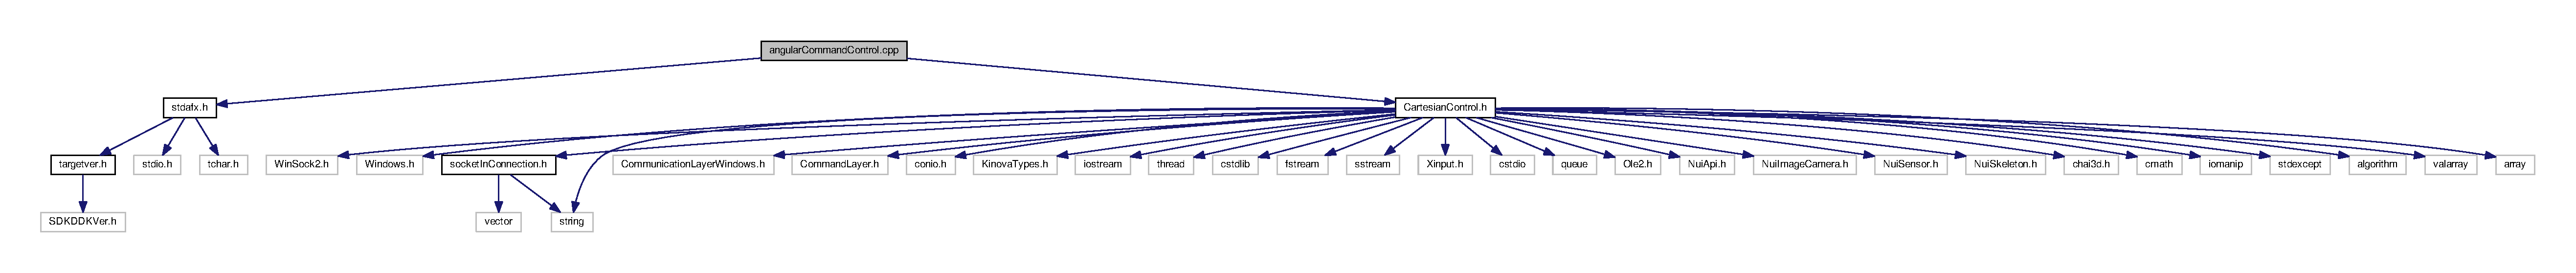
\includegraphics[width=350pt]{da/d87/angularCommandControl_8cpp__incl}
\end{center}
\end{figure}
\subsection*{Macros}
\begin{DoxyCompactItemize}
\item 
\#define \hyperlink{angularCommandControl_8cpp_adfc8f90f3a8caa8423099cf36ff214f1}{\+\_\+\+W\+I\+N\+S\+O\+C\+K\+\_\+\+D\+E\+P\+R\+E\+C\+A\+T\+E\+D\+\_\+\+N\+O\+\_\+\+W\+A\+R\+N\+I\+N\+GS}
\item 
\#define \hyperlink{angularCommandControl_8cpp_ac7bef5d85e3dcd73eef56ad39ffc84a9}{W\+I\+N32\+\_\+\+L\+E\+A\+N\+\_\+\+A\+N\+D\+\_\+\+M\+E\+AN}
\end{DoxyCompactItemize}


\subsection{Macro Definition Documentation}
\index{angular\+Command\+Control.\+cpp@{angular\+Command\+Control.\+cpp}!\+\_\+\+W\+I\+N\+S\+O\+C\+K\+\_\+\+D\+E\+P\+R\+E\+C\+A\+T\+E\+D\+\_\+\+N\+O\+\_\+\+W\+A\+R\+N\+I\+N\+GS@{\+\_\+\+W\+I\+N\+S\+O\+C\+K\+\_\+\+D\+E\+P\+R\+E\+C\+A\+T\+E\+D\+\_\+\+N\+O\+\_\+\+W\+A\+R\+N\+I\+N\+GS}}
\index{\+\_\+\+W\+I\+N\+S\+O\+C\+K\+\_\+\+D\+E\+P\+R\+E\+C\+A\+T\+E\+D\+\_\+\+N\+O\+\_\+\+W\+A\+R\+N\+I\+N\+GS@{\+\_\+\+W\+I\+N\+S\+O\+C\+K\+\_\+\+D\+E\+P\+R\+E\+C\+A\+T\+E\+D\+\_\+\+N\+O\+\_\+\+W\+A\+R\+N\+I\+N\+GS}!angular\+Command\+Control.\+cpp@{angular\+Command\+Control.\+cpp}}
\subsubsection[{\texorpdfstring{\+\_\+\+W\+I\+N\+S\+O\+C\+K\+\_\+\+D\+E\+P\+R\+E\+C\+A\+T\+E\+D\+\_\+\+N\+O\+\_\+\+W\+A\+R\+N\+I\+N\+GS}{_WINSOCK_DEPRECATED_NO_WARNINGS}}]{\setlength{\rightskip}{0pt plus 5cm}\#define \+\_\+\+W\+I\+N\+S\+O\+C\+K\+\_\+\+D\+E\+P\+R\+E\+C\+A\+T\+E\+D\+\_\+\+N\+O\+\_\+\+W\+A\+R\+N\+I\+N\+GS}\hypertarget{angularCommandControl_8cpp_adfc8f90f3a8caa8423099cf36ff214f1}{}\label{angularCommandControl_8cpp_adfc8f90f3a8caa8423099cf36ff214f1}
\index{angular\+Command\+Control.\+cpp@{angular\+Command\+Control.\+cpp}!W\+I\+N32\+\_\+\+L\+E\+A\+N\+\_\+\+A\+N\+D\+\_\+\+M\+E\+AN@{W\+I\+N32\+\_\+\+L\+E\+A\+N\+\_\+\+A\+N\+D\+\_\+\+M\+E\+AN}}
\index{W\+I\+N32\+\_\+\+L\+E\+A\+N\+\_\+\+A\+N\+D\+\_\+\+M\+E\+AN@{W\+I\+N32\+\_\+\+L\+E\+A\+N\+\_\+\+A\+N\+D\+\_\+\+M\+E\+AN}!angular\+Command\+Control.\+cpp@{angular\+Command\+Control.\+cpp}}
\subsubsection[{\texorpdfstring{W\+I\+N32\+\_\+\+L\+E\+A\+N\+\_\+\+A\+N\+D\+\_\+\+M\+E\+AN}{WIN32_LEAN_AND_MEAN}}]{\setlength{\rightskip}{0pt plus 5cm}\#define W\+I\+N32\+\_\+\+L\+E\+A\+N\+\_\+\+A\+N\+D\+\_\+\+M\+E\+AN}\hypertarget{angularCommandControl_8cpp_ac7bef5d85e3dcd73eef56ad39ffc84a9}{}\label{angularCommandControl_8cpp_ac7bef5d85e3dcd73eef56ad39ffc84a9}

\hypertarget{CartesianControl_8h}{}\section{Cartesian\+Control.\+h File Reference}
\label{CartesianControl_8h}\index{Cartesian\+Control.\+h@{Cartesian\+Control.\+h}}
{\ttfamily \#include $<$Win\+Sock2.\+h$>$}\\*
{\ttfamily \#include $<$Windows.\+h$>$}\\*
{\ttfamily \#include \char`\"{}socket\+In\+Connection.\+h\char`\"{}}\\*
{\ttfamily \#include \char`\"{}Communication\+Layer\+Windows.\+h\char`\"{}}\\*
{\ttfamily \#include \char`\"{}Command\+Layer.\+h\char`\"{}}\\*
{\ttfamily \#include $<$conio.\+h$>$}\\*
{\ttfamily \#include \char`\"{}Kinova\+Types.\+h\char`\"{}}\\*
{\ttfamily \#include $<$iostream$>$}\\*
{\ttfamily \#include $<$thread$>$}\\*
{\ttfamily \#include $<$cstdlib$>$}\\*
{\ttfamily \#include $<$fstream$>$}\\*
{\ttfamily \#include $<$string$>$}\\*
{\ttfamily \#include $<$sstream$>$}\\*
{\ttfamily \#include $<$Xinput.\+h$>$}\\*
{\ttfamily \#include $<$cstdio$>$}\\*
{\ttfamily \#include $<$queue$>$}\\*
{\ttfamily \#include $<$Ole2.\+h$>$}\\*
{\ttfamily \#include \char`\"{}Nui\+Api.\+h\char`\"{}}\\*
{\ttfamily \#include \char`\"{}Nui\+Image\+Camera.\+h\char`\"{}}\\*
{\ttfamily \#include \char`\"{}Nui\+Sensor.\+h\char`\"{}}\\*
{\ttfamily \#include \char`\"{}Nui\+Skeleton.\+h\char`\"{}}\\*
{\ttfamily \#include \char`\"{}chai3d.\+h\char`\"{}}\\*
{\ttfamily \#include $<$cmath$>$}\\*
{\ttfamily \#include $<$iomanip$>$}\\*
{\ttfamily \#include $<$stdexcept$>$}\\*
{\ttfamily \#include $<$algorithm$>$}\\*
{\ttfamily \#include $<$valarray$>$}\\*
{\ttfamily \#include $<$array$>$}\\*
Include dependency graph for Cartesian\+Control.\+h\+:\nopagebreak
\begin{figure}[H]
\begin{center}
\leavevmode
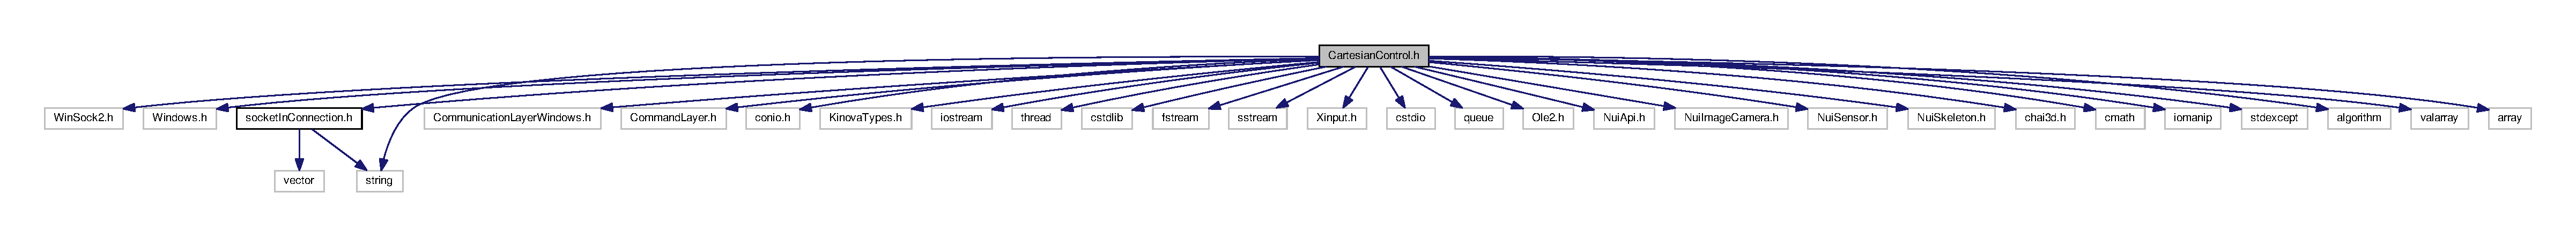
\includegraphics[width=350pt]{d0/d3f/CartesianControl_8h__incl}
\end{center}
\end{figure}
This graph shows which files directly or indirectly include this file\+:\nopagebreak
\begin{figure}[H]
\begin{center}
\leavevmode
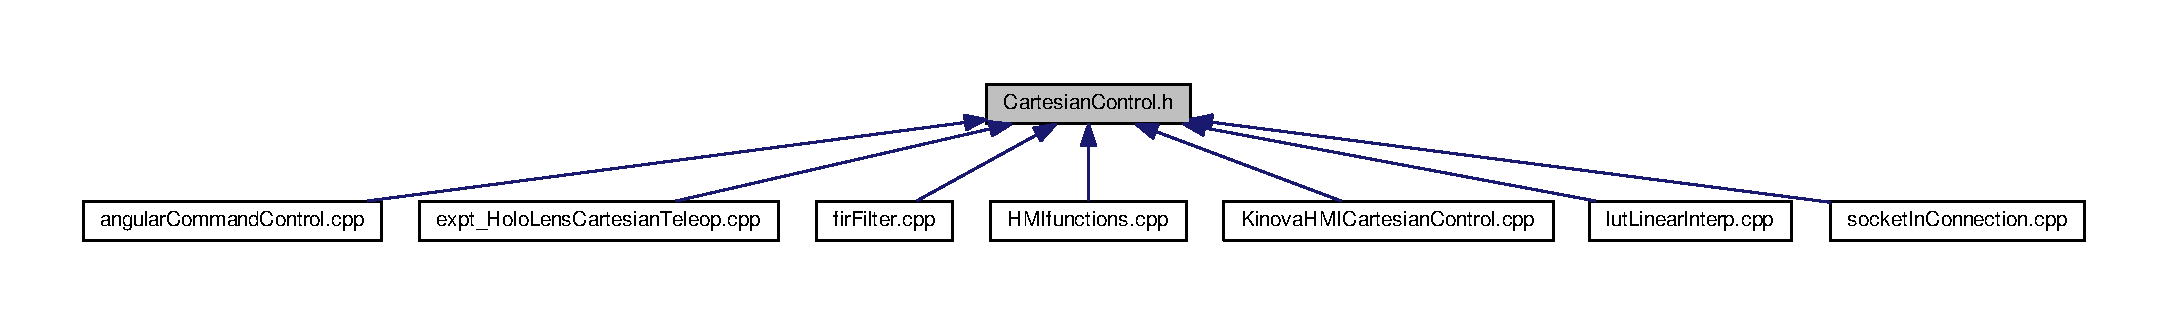
\includegraphics[width=350pt]{d3/d8d/CartesianControl_8h__dep__incl}
\end{center}
\end{figure}
\subsection*{Classes}
\begin{DoxyCompactItemize}
\item 
class \hyperlink{classCXBOXController}{C\+X\+B\+O\+X\+Controller}
\item 
class \hyperlink{classTimer}{Timer}
\item 
class \hyperlink{classKinovaAPIFunctions}{Kinova\+A\+P\+I\+Functions}
\item 
class \hyperlink{classkinectSkelTrack}{kinect\+Skel\+Track}
\item 
struct \hyperlink{structkinectSkelTrack_1_1KinectInfo}{kinect\+Skel\+Track\+::\+Kinect\+Info}
\item 
class \hyperlink{classFIRFilter}{F\+I\+R\+Filter}
\item 
class \hyperlink{classExperiment}{Experiment}
\item 
class \hyperlink{classNovintFalconHapticsDevice}{Novint\+Falcon\+Haptics\+Device}
\end{DoxyCompactItemize}
\subsection*{Macros}
\begin{DoxyCompactItemize}
\item 
\#define \hyperlink{CartesianControl_8h_adfc8f90f3a8caa8423099cf36ff214f1}{\+\_\+\+W\+I\+N\+S\+O\+C\+K\+\_\+\+D\+E\+P\+R\+E\+C\+A\+T\+E\+D\+\_\+\+N\+O\+\_\+\+W\+A\+R\+N\+I\+N\+GS}
\item 
\#define \hyperlink{CartesianControl_8h_ac7bef5d85e3dcd73eef56ad39ffc84a9}{W\+I\+N32\+\_\+\+L\+E\+A\+N\+\_\+\+A\+N\+D\+\_\+\+M\+E\+AN}
\item 
\#define \hyperlink{CartesianControl_8h_ac7bef5d85e3dcd73eef56ad39ffc84a9}{W\+I\+N32\+\_\+\+L\+E\+A\+N\+\_\+\+A\+N\+D\+\_\+\+M\+E\+AN}
\item 
\#define \hyperlink{CartesianControl_8h_a0934169ae417a287adfd19bdd7a13137}{U\+S\+E\+\_\+\+K\+I\+N\+O\+VA}~true
\item 
\#define \hyperlink{CartesianControl_8h_a4b87829c8dfd2ba03fdc55f059b87bef}{U\+S\+E\+\_\+\+K\+I\+N\+E\+CT}~false
\item 
\#define \hyperlink{CartesianControl_8h_a1a02ac5217ce78990cacecfae4f6d509}{U\+S\+E\+\_\+\+T\+CP}~true
\item 
\#define \hyperlink{CartesianControl_8h_ad15cf97d77a6dd54ab0e2c90387bcb0b}{U\+S\+E\+\_\+\+H\+A\+P\+T\+I\+CS}~true
\item 
\#define \hyperlink{CartesianControl_8h_aec53ee0acd16d9f951bc2f63235fa914}{G\+N\+U\+P\+L\+OT}~false
\item 
\#define \hyperlink{CartesianControl_8h_a889394d13af6d709e557cdc4a16db344}{\+\_\+\+X\+B\+O\+X\+\_\+\+C\+O\+N\+T\+R\+O\+L\+L\+E\+R\+\_\+\+H\+\_\+}
\item 
\#define \hyperlink{CartesianControl_8h_ac7bef5d85e3dcd73eef56ad39ffc84a9}{W\+I\+N32\+\_\+\+L\+E\+A\+N\+\_\+\+A\+N\+D\+\_\+\+M\+E\+AN}
\item 
\#define \hyperlink{CartesianControl_8h_a46130dc86f2322714bba26960b64e7bb}{B\+U\+F\+F\+E\+R\+\_\+\+L\+EN}~96
\begin{DoxyCompactList}\small\item\em Buffer length to hold input samples of F\+IR Filter. \end{DoxyCompactList}\end{DoxyCompactItemize}


\subsection{Macro Definition Documentation}
\index{Cartesian\+Control.\+h@{Cartesian\+Control.\+h}!\+\_\+\+W\+I\+N\+S\+O\+C\+K\+\_\+\+D\+E\+P\+R\+E\+C\+A\+T\+E\+D\+\_\+\+N\+O\+\_\+\+W\+A\+R\+N\+I\+N\+GS@{\+\_\+\+W\+I\+N\+S\+O\+C\+K\+\_\+\+D\+E\+P\+R\+E\+C\+A\+T\+E\+D\+\_\+\+N\+O\+\_\+\+W\+A\+R\+N\+I\+N\+GS}}
\index{\+\_\+\+W\+I\+N\+S\+O\+C\+K\+\_\+\+D\+E\+P\+R\+E\+C\+A\+T\+E\+D\+\_\+\+N\+O\+\_\+\+W\+A\+R\+N\+I\+N\+GS@{\+\_\+\+W\+I\+N\+S\+O\+C\+K\+\_\+\+D\+E\+P\+R\+E\+C\+A\+T\+E\+D\+\_\+\+N\+O\+\_\+\+W\+A\+R\+N\+I\+N\+GS}!Cartesian\+Control.\+h@{Cartesian\+Control.\+h}}
\subsubsection[{\texorpdfstring{\+\_\+\+W\+I\+N\+S\+O\+C\+K\+\_\+\+D\+E\+P\+R\+E\+C\+A\+T\+E\+D\+\_\+\+N\+O\+\_\+\+W\+A\+R\+N\+I\+N\+GS}{_WINSOCK_DEPRECATED_NO_WARNINGS}}]{\setlength{\rightskip}{0pt plus 5cm}\#define \+\_\+\+W\+I\+N\+S\+O\+C\+K\+\_\+\+D\+E\+P\+R\+E\+C\+A\+T\+E\+D\+\_\+\+N\+O\+\_\+\+W\+A\+R\+N\+I\+N\+GS}\hypertarget{CartesianControl_8h_adfc8f90f3a8caa8423099cf36ff214f1}{}\label{CartesianControl_8h_adfc8f90f3a8caa8423099cf36ff214f1}
\index{Cartesian\+Control.\+h@{Cartesian\+Control.\+h}!\+\_\+\+X\+B\+O\+X\+\_\+\+C\+O\+N\+T\+R\+O\+L\+L\+E\+R\+\_\+\+H\+\_\+@{\+\_\+\+X\+B\+O\+X\+\_\+\+C\+O\+N\+T\+R\+O\+L\+L\+E\+R\+\_\+\+H\+\_\+}}
\index{\+\_\+\+X\+B\+O\+X\+\_\+\+C\+O\+N\+T\+R\+O\+L\+L\+E\+R\+\_\+\+H\+\_\+@{\+\_\+\+X\+B\+O\+X\+\_\+\+C\+O\+N\+T\+R\+O\+L\+L\+E\+R\+\_\+\+H\+\_\+}!Cartesian\+Control.\+h@{Cartesian\+Control.\+h}}
\subsubsection[{\texorpdfstring{\+\_\+\+X\+B\+O\+X\+\_\+\+C\+O\+N\+T\+R\+O\+L\+L\+E\+R\+\_\+\+H\+\_\+}{_XBOX_CONTROLLER_H_}}]{\setlength{\rightskip}{0pt plus 5cm}\#define \+\_\+\+X\+B\+O\+X\+\_\+\+C\+O\+N\+T\+R\+O\+L\+L\+E\+R\+\_\+\+H\+\_\+}\hypertarget{CartesianControl_8h_a889394d13af6d709e557cdc4a16db344}{}\label{CartesianControl_8h_a889394d13af6d709e557cdc4a16db344}
\index{Cartesian\+Control.\+h@{Cartesian\+Control.\+h}!B\+U\+F\+F\+E\+R\+\_\+\+L\+EN@{B\+U\+F\+F\+E\+R\+\_\+\+L\+EN}}
\index{B\+U\+F\+F\+E\+R\+\_\+\+L\+EN@{B\+U\+F\+F\+E\+R\+\_\+\+L\+EN}!Cartesian\+Control.\+h@{Cartesian\+Control.\+h}}
\subsubsection[{\texorpdfstring{B\+U\+F\+F\+E\+R\+\_\+\+L\+EN}{BUFFER_LEN}}]{\setlength{\rightskip}{0pt plus 5cm}\#define B\+U\+F\+F\+E\+R\+\_\+\+L\+EN~96}\hypertarget{CartesianControl_8h_a46130dc86f2322714bba26960b64e7bb}{}\label{CartesianControl_8h_a46130dc86f2322714bba26960b64e7bb}


Buffer length to hold input samples of F\+IR Filter. 

\index{Cartesian\+Control.\+h@{Cartesian\+Control.\+h}!G\+N\+U\+P\+L\+OT@{G\+N\+U\+P\+L\+OT}}
\index{G\+N\+U\+P\+L\+OT@{G\+N\+U\+P\+L\+OT}!Cartesian\+Control.\+h@{Cartesian\+Control.\+h}}
\subsubsection[{\texorpdfstring{G\+N\+U\+P\+L\+OT}{GNUPLOT}}]{\setlength{\rightskip}{0pt plus 5cm}\#define G\+N\+U\+P\+L\+OT~false}\hypertarget{CartesianControl_8h_aec53ee0acd16d9f951bc2f63235fa914}{}\label{CartesianControl_8h_aec53ee0acd16d9f951bc2f63235fa914}
\index{Cartesian\+Control.\+h@{Cartesian\+Control.\+h}!U\+S\+E\+\_\+\+H\+A\+P\+T\+I\+CS@{U\+S\+E\+\_\+\+H\+A\+P\+T\+I\+CS}}
\index{U\+S\+E\+\_\+\+H\+A\+P\+T\+I\+CS@{U\+S\+E\+\_\+\+H\+A\+P\+T\+I\+CS}!Cartesian\+Control.\+h@{Cartesian\+Control.\+h}}
\subsubsection[{\texorpdfstring{U\+S\+E\+\_\+\+H\+A\+P\+T\+I\+CS}{USE_HAPTICS}}]{\setlength{\rightskip}{0pt plus 5cm}\#define U\+S\+E\+\_\+\+H\+A\+P\+T\+I\+CS~true}\hypertarget{CartesianControl_8h_ad15cf97d77a6dd54ab0e2c90387bcb0b}{}\label{CartesianControl_8h_ad15cf97d77a6dd54ab0e2c90387bcb0b}
\index{Cartesian\+Control.\+h@{Cartesian\+Control.\+h}!U\+S\+E\+\_\+\+K\+I\+N\+E\+CT@{U\+S\+E\+\_\+\+K\+I\+N\+E\+CT}}
\index{U\+S\+E\+\_\+\+K\+I\+N\+E\+CT@{U\+S\+E\+\_\+\+K\+I\+N\+E\+CT}!Cartesian\+Control.\+h@{Cartesian\+Control.\+h}}
\subsubsection[{\texorpdfstring{U\+S\+E\+\_\+\+K\+I\+N\+E\+CT}{USE_KINECT}}]{\setlength{\rightskip}{0pt plus 5cm}\#define U\+S\+E\+\_\+\+K\+I\+N\+E\+CT~false}\hypertarget{CartesianControl_8h_a4b87829c8dfd2ba03fdc55f059b87bef}{}\label{CartesianControl_8h_a4b87829c8dfd2ba03fdc55f059b87bef}
\index{Cartesian\+Control.\+h@{Cartesian\+Control.\+h}!U\+S\+E\+\_\+\+K\+I\+N\+O\+VA@{U\+S\+E\+\_\+\+K\+I\+N\+O\+VA}}
\index{U\+S\+E\+\_\+\+K\+I\+N\+O\+VA@{U\+S\+E\+\_\+\+K\+I\+N\+O\+VA}!Cartesian\+Control.\+h@{Cartesian\+Control.\+h}}
\subsubsection[{\texorpdfstring{U\+S\+E\+\_\+\+K\+I\+N\+O\+VA}{USE_KINOVA}}]{\setlength{\rightskip}{0pt plus 5cm}\#define U\+S\+E\+\_\+\+K\+I\+N\+O\+VA~true}\hypertarget{CartesianControl_8h_a0934169ae417a287adfd19bdd7a13137}{}\label{CartesianControl_8h_a0934169ae417a287adfd19bdd7a13137}
\index{Cartesian\+Control.\+h@{Cartesian\+Control.\+h}!U\+S\+E\+\_\+\+T\+CP@{U\+S\+E\+\_\+\+T\+CP}}
\index{U\+S\+E\+\_\+\+T\+CP@{U\+S\+E\+\_\+\+T\+CP}!Cartesian\+Control.\+h@{Cartesian\+Control.\+h}}
\subsubsection[{\texorpdfstring{U\+S\+E\+\_\+\+T\+CP}{USE_TCP}}]{\setlength{\rightskip}{0pt plus 5cm}\#define U\+S\+E\+\_\+\+T\+CP~true}\hypertarget{CartesianControl_8h_a1a02ac5217ce78990cacecfae4f6d509}{}\label{CartesianControl_8h_a1a02ac5217ce78990cacecfae4f6d509}
\index{Cartesian\+Control.\+h@{Cartesian\+Control.\+h}!W\+I\+N32\+\_\+\+L\+E\+A\+N\+\_\+\+A\+N\+D\+\_\+\+M\+E\+AN@{W\+I\+N32\+\_\+\+L\+E\+A\+N\+\_\+\+A\+N\+D\+\_\+\+M\+E\+AN}}
\index{W\+I\+N32\+\_\+\+L\+E\+A\+N\+\_\+\+A\+N\+D\+\_\+\+M\+E\+AN@{W\+I\+N32\+\_\+\+L\+E\+A\+N\+\_\+\+A\+N\+D\+\_\+\+M\+E\+AN}!Cartesian\+Control.\+h@{Cartesian\+Control.\+h}}
\subsubsection[{\texorpdfstring{W\+I\+N32\+\_\+\+L\+E\+A\+N\+\_\+\+A\+N\+D\+\_\+\+M\+E\+AN}{WIN32_LEAN_AND_MEAN}}]{\setlength{\rightskip}{0pt plus 5cm}\#define W\+I\+N32\+\_\+\+L\+E\+A\+N\+\_\+\+A\+N\+D\+\_\+\+M\+E\+AN}\hypertarget{CartesianControl_8h_ac7bef5d85e3dcd73eef56ad39ffc84a9}{}\label{CartesianControl_8h_ac7bef5d85e3dcd73eef56ad39ffc84a9}
\index{Cartesian\+Control.\+h@{Cartesian\+Control.\+h}!W\+I\+N32\+\_\+\+L\+E\+A\+N\+\_\+\+A\+N\+D\+\_\+\+M\+E\+AN@{W\+I\+N32\+\_\+\+L\+E\+A\+N\+\_\+\+A\+N\+D\+\_\+\+M\+E\+AN}}
\index{W\+I\+N32\+\_\+\+L\+E\+A\+N\+\_\+\+A\+N\+D\+\_\+\+M\+E\+AN@{W\+I\+N32\+\_\+\+L\+E\+A\+N\+\_\+\+A\+N\+D\+\_\+\+M\+E\+AN}!Cartesian\+Control.\+h@{Cartesian\+Control.\+h}}
\subsubsection[{\texorpdfstring{W\+I\+N32\+\_\+\+L\+E\+A\+N\+\_\+\+A\+N\+D\+\_\+\+M\+E\+AN}{WIN32_LEAN_AND_MEAN}}]{\setlength{\rightskip}{0pt plus 5cm}\#define W\+I\+N32\+\_\+\+L\+E\+A\+N\+\_\+\+A\+N\+D\+\_\+\+M\+E\+AN}\hypertarget{CartesianControl_8h_ac7bef5d85e3dcd73eef56ad39ffc84a9}{}\label{CartesianControl_8h_ac7bef5d85e3dcd73eef56ad39ffc84a9}
\index{Cartesian\+Control.\+h@{Cartesian\+Control.\+h}!W\+I\+N32\+\_\+\+L\+E\+A\+N\+\_\+\+A\+N\+D\+\_\+\+M\+E\+AN@{W\+I\+N32\+\_\+\+L\+E\+A\+N\+\_\+\+A\+N\+D\+\_\+\+M\+E\+AN}}
\index{W\+I\+N32\+\_\+\+L\+E\+A\+N\+\_\+\+A\+N\+D\+\_\+\+M\+E\+AN@{W\+I\+N32\+\_\+\+L\+E\+A\+N\+\_\+\+A\+N\+D\+\_\+\+M\+E\+AN}!Cartesian\+Control.\+h@{Cartesian\+Control.\+h}}
\subsubsection[{\texorpdfstring{W\+I\+N32\+\_\+\+L\+E\+A\+N\+\_\+\+A\+N\+D\+\_\+\+M\+E\+AN}{WIN32_LEAN_AND_MEAN}}]{\setlength{\rightskip}{0pt plus 5cm}\#define W\+I\+N32\+\_\+\+L\+E\+A\+N\+\_\+\+A\+N\+D\+\_\+\+M\+E\+AN}\hypertarget{CartesianControl_8h_ac7bef5d85e3dcd73eef56ad39ffc84a9}{}\label{CartesianControl_8h_ac7bef5d85e3dcd73eef56ad39ffc84a9}

\hypertarget{expt__HoloLensCartesianTeleop_8cpp}{}\section{expt\+\_\+\+Holo\+Lens\+Cartesian\+Teleop.\+cpp File Reference}
\label{expt__HoloLensCartesianTeleop_8cpp}\index{expt\+\_\+\+Holo\+Lens\+Cartesian\+Teleop.\+cpp@{expt\+\_\+\+Holo\+Lens\+Cartesian\+Teleop.\+cpp}}
{\ttfamily \#include \char`\"{}stdafx.\+h\char`\"{}}\\*
{\ttfamily \#include \char`\"{}Cartesian\+Control.\+h\char`\"{}}\\*
{\ttfamily \#include $<$vector$>$}\\*
{\ttfamily \#include $<$queue$>$}\\*
{\ttfamily \#include $<$future$>$}\\*
Include dependency graph for expt\+\_\+\+Holo\+Lens\+Cartesian\+Teleop.\+cpp\+:\nopagebreak
\begin{figure}[H]
\begin{center}
\leavevmode
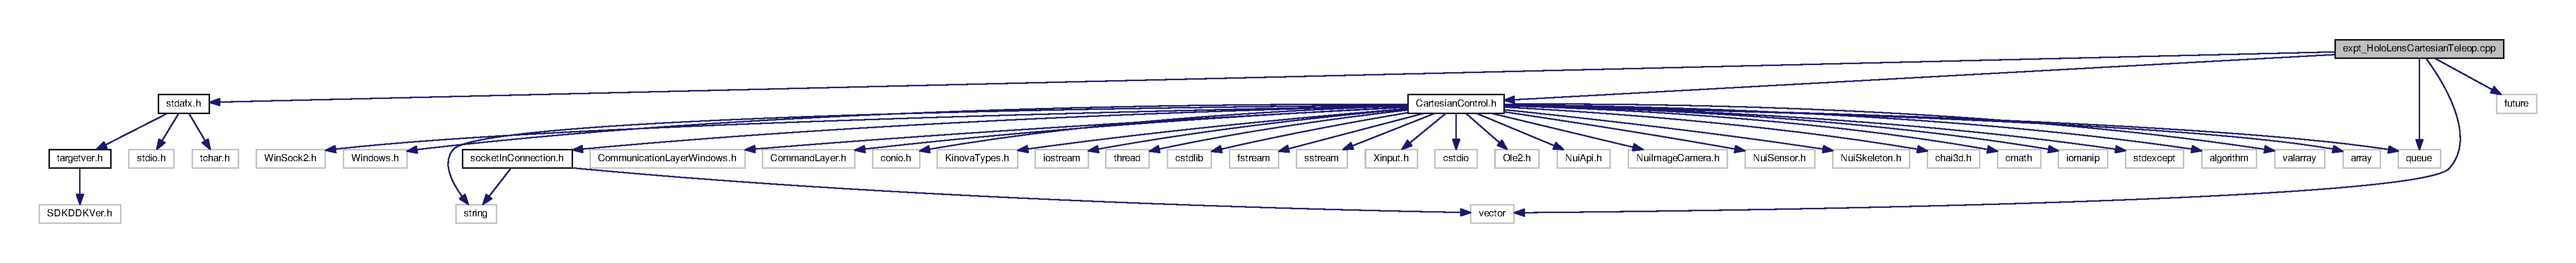
\includegraphics[width=350pt]{da/d5b/expt__HoloLensCartesianTeleop_8cpp__incl}
\end{center}
\end{figure}
\subsection*{Macros}
\begin{DoxyCompactItemize}
\item 
\#define \hyperlink{expt__HoloLensCartesianTeleop_8cpp_a5762b99b606a8008d4244c4d484e1f1c}{T\+R\+A\+IN}~true
\item 
\#define \hyperlink{expt__HoloLensCartesianTeleop_8cpp_a864a52c772f23a04bcef46a40c9efed4}{T\+E\+S\+T\+\_\+1}~false
\item 
\#define \hyperlink{expt__HoloLensCartesianTeleop_8cpp_aa97013921b0b86f7b58de46505cd223b}{T\+E\+S\+T\+\_\+2}~false
\item 
\#define \hyperlink{expt__HoloLensCartesianTeleop_8cpp_ac86054dc8d23e66c9556657b04e2a5f3}{I\+N\+V\+E\+R\+S\+E\+\_\+\+C\+O\+N\+T\+R\+O\+L\+L\+ER}~false
\item 
\#define \hyperlink{expt__HoloLensCartesianTeleop_8cpp_ace138276390387cfa2180f589e502f82}{L\+O\+A\+D\+\_\+\+U\+H\+X\+\_\+\+F\+R\+O\+M\+\_\+\+F\+I\+LE}~false
\item 
\#define \hyperlink{expt__HoloLensCartesianTeleop_8cpp_a0d517e64a65ae6a5522a96096b29ee6b}{L\+O\+A\+D\+\_\+\+X\+M\+\_\+\+F\+R\+O\+M\+\_\+\+F\+I\+LE}~false
\end{DoxyCompactItemize}
\subsection*{Variables}
\begin{DoxyCompactItemize}
\item 
\hyperlink{classNovintFalconHapticsDevice}{Novint\+Falcon\+Haptics\+Device} $\ast$ \hyperlink{expt__HoloLensCartesianTeleop_8cpp_a5af8a150b7e3676a29b7844262dd4d6f}{novint\+Falcon} = new \hyperlink{classNovintFalconHapticsDevice}{Novint\+Falcon\+Haptics\+Device}
\end{DoxyCompactItemize}


\subsection{Macro Definition Documentation}
\index{expt\+\_\+\+Holo\+Lens\+Cartesian\+Teleop.\+cpp@{expt\+\_\+\+Holo\+Lens\+Cartesian\+Teleop.\+cpp}!I\+N\+V\+E\+R\+S\+E\+\_\+\+C\+O\+N\+T\+R\+O\+L\+L\+ER@{I\+N\+V\+E\+R\+S\+E\+\_\+\+C\+O\+N\+T\+R\+O\+L\+L\+ER}}
\index{I\+N\+V\+E\+R\+S\+E\+\_\+\+C\+O\+N\+T\+R\+O\+L\+L\+ER@{I\+N\+V\+E\+R\+S\+E\+\_\+\+C\+O\+N\+T\+R\+O\+L\+L\+ER}!expt\+\_\+\+Holo\+Lens\+Cartesian\+Teleop.\+cpp@{expt\+\_\+\+Holo\+Lens\+Cartesian\+Teleop.\+cpp}}
\subsubsection[{\texorpdfstring{I\+N\+V\+E\+R\+S\+E\+\_\+\+C\+O\+N\+T\+R\+O\+L\+L\+ER}{INVERSE_CONTROLLER}}]{\setlength{\rightskip}{0pt plus 5cm}\#define I\+N\+V\+E\+R\+S\+E\+\_\+\+C\+O\+N\+T\+R\+O\+L\+L\+ER~false}\hypertarget{expt__HoloLensCartesianTeleop_8cpp_ac86054dc8d23e66c9556657b04e2a5f3}{}\label{expt__HoloLensCartesianTeleop_8cpp_ac86054dc8d23e66c9556657b04e2a5f3}
\index{expt\+\_\+\+Holo\+Lens\+Cartesian\+Teleop.\+cpp@{expt\+\_\+\+Holo\+Lens\+Cartesian\+Teleop.\+cpp}!L\+O\+A\+D\+\_\+\+U\+H\+X\+\_\+\+F\+R\+O\+M\+\_\+\+F\+I\+LE@{L\+O\+A\+D\+\_\+\+U\+H\+X\+\_\+\+F\+R\+O\+M\+\_\+\+F\+I\+LE}}
\index{L\+O\+A\+D\+\_\+\+U\+H\+X\+\_\+\+F\+R\+O\+M\+\_\+\+F\+I\+LE@{L\+O\+A\+D\+\_\+\+U\+H\+X\+\_\+\+F\+R\+O\+M\+\_\+\+F\+I\+LE}!expt\+\_\+\+Holo\+Lens\+Cartesian\+Teleop.\+cpp@{expt\+\_\+\+Holo\+Lens\+Cartesian\+Teleop.\+cpp}}
\subsubsection[{\texorpdfstring{L\+O\+A\+D\+\_\+\+U\+H\+X\+\_\+\+F\+R\+O\+M\+\_\+\+F\+I\+LE}{LOAD_UHX_FROM_FILE}}]{\setlength{\rightskip}{0pt plus 5cm}\#define L\+O\+A\+D\+\_\+\+U\+H\+X\+\_\+\+F\+R\+O\+M\+\_\+\+F\+I\+LE~false}\hypertarget{expt__HoloLensCartesianTeleop_8cpp_ace138276390387cfa2180f589e502f82}{}\label{expt__HoloLensCartesianTeleop_8cpp_ace138276390387cfa2180f589e502f82}
\index{expt\+\_\+\+Holo\+Lens\+Cartesian\+Teleop.\+cpp@{expt\+\_\+\+Holo\+Lens\+Cartesian\+Teleop.\+cpp}!L\+O\+A\+D\+\_\+\+X\+M\+\_\+\+F\+R\+O\+M\+\_\+\+F\+I\+LE@{L\+O\+A\+D\+\_\+\+X\+M\+\_\+\+F\+R\+O\+M\+\_\+\+F\+I\+LE}}
\index{L\+O\+A\+D\+\_\+\+X\+M\+\_\+\+F\+R\+O\+M\+\_\+\+F\+I\+LE@{L\+O\+A\+D\+\_\+\+X\+M\+\_\+\+F\+R\+O\+M\+\_\+\+F\+I\+LE}!expt\+\_\+\+Holo\+Lens\+Cartesian\+Teleop.\+cpp@{expt\+\_\+\+Holo\+Lens\+Cartesian\+Teleop.\+cpp}}
\subsubsection[{\texorpdfstring{L\+O\+A\+D\+\_\+\+X\+M\+\_\+\+F\+R\+O\+M\+\_\+\+F\+I\+LE}{LOAD_XM_FROM_FILE}}]{\setlength{\rightskip}{0pt plus 5cm}\#define L\+O\+A\+D\+\_\+\+X\+M\+\_\+\+F\+R\+O\+M\+\_\+\+F\+I\+LE~false}\hypertarget{expt__HoloLensCartesianTeleop_8cpp_a0d517e64a65ae6a5522a96096b29ee6b}{}\label{expt__HoloLensCartesianTeleop_8cpp_a0d517e64a65ae6a5522a96096b29ee6b}
\index{expt\+\_\+\+Holo\+Lens\+Cartesian\+Teleop.\+cpp@{expt\+\_\+\+Holo\+Lens\+Cartesian\+Teleop.\+cpp}!T\+E\+S\+T\+\_\+1@{T\+E\+S\+T\+\_\+1}}
\index{T\+E\+S\+T\+\_\+1@{T\+E\+S\+T\+\_\+1}!expt\+\_\+\+Holo\+Lens\+Cartesian\+Teleop.\+cpp@{expt\+\_\+\+Holo\+Lens\+Cartesian\+Teleop.\+cpp}}
\subsubsection[{\texorpdfstring{T\+E\+S\+T\+\_\+1}{TEST_1}}]{\setlength{\rightskip}{0pt plus 5cm}\#define T\+E\+S\+T\+\_\+1~false}\hypertarget{expt__HoloLensCartesianTeleop_8cpp_a864a52c772f23a04bcef46a40c9efed4}{}\label{expt__HoloLensCartesianTeleop_8cpp_a864a52c772f23a04bcef46a40c9efed4}
\index{expt\+\_\+\+Holo\+Lens\+Cartesian\+Teleop.\+cpp@{expt\+\_\+\+Holo\+Lens\+Cartesian\+Teleop.\+cpp}!T\+E\+S\+T\+\_\+2@{T\+E\+S\+T\+\_\+2}}
\index{T\+E\+S\+T\+\_\+2@{T\+E\+S\+T\+\_\+2}!expt\+\_\+\+Holo\+Lens\+Cartesian\+Teleop.\+cpp@{expt\+\_\+\+Holo\+Lens\+Cartesian\+Teleop.\+cpp}}
\subsubsection[{\texorpdfstring{T\+E\+S\+T\+\_\+2}{TEST_2}}]{\setlength{\rightskip}{0pt plus 5cm}\#define T\+E\+S\+T\+\_\+2~false}\hypertarget{expt__HoloLensCartesianTeleop_8cpp_aa97013921b0b86f7b58de46505cd223b}{}\label{expt__HoloLensCartesianTeleop_8cpp_aa97013921b0b86f7b58de46505cd223b}
\index{expt\+\_\+\+Holo\+Lens\+Cartesian\+Teleop.\+cpp@{expt\+\_\+\+Holo\+Lens\+Cartesian\+Teleop.\+cpp}!T\+R\+A\+IN@{T\+R\+A\+IN}}
\index{T\+R\+A\+IN@{T\+R\+A\+IN}!expt\+\_\+\+Holo\+Lens\+Cartesian\+Teleop.\+cpp@{expt\+\_\+\+Holo\+Lens\+Cartesian\+Teleop.\+cpp}}
\subsubsection[{\texorpdfstring{T\+R\+A\+IN}{TRAIN}}]{\setlength{\rightskip}{0pt plus 5cm}\#define T\+R\+A\+IN~true}\hypertarget{expt__HoloLensCartesianTeleop_8cpp_a5762b99b606a8008d4244c4d484e1f1c}{}\label{expt__HoloLensCartesianTeleop_8cpp_a5762b99b606a8008d4244c4d484e1f1c}


\subsection{Variable Documentation}
\index{expt\+\_\+\+Holo\+Lens\+Cartesian\+Teleop.\+cpp@{expt\+\_\+\+Holo\+Lens\+Cartesian\+Teleop.\+cpp}!novint\+Falcon@{novint\+Falcon}}
\index{novint\+Falcon@{novint\+Falcon}!expt\+\_\+\+Holo\+Lens\+Cartesian\+Teleop.\+cpp@{expt\+\_\+\+Holo\+Lens\+Cartesian\+Teleop.\+cpp}}
\subsubsection[{\texorpdfstring{novint\+Falcon}{novintFalcon}}]{\setlength{\rightskip}{0pt plus 5cm}{\bf Novint\+Falcon\+Haptics\+Device}$\ast$ novint\+Falcon = new {\bf Novint\+Falcon\+Haptics\+Device}}\hypertarget{expt__HoloLensCartesianTeleop_8cpp_a5af8a150b7e3676a29b7844262dd4d6f}{}\label{expt__HoloLensCartesianTeleop_8cpp_a5af8a150b7e3676a29b7844262dd4d6f}

\hypertarget{firFilter_8cpp}{}\section{fir\+Filter.\+cpp File Reference}
\label{firFilter_8cpp}\index{fir\+Filter.\+cpp@{fir\+Filter.\+cpp}}
{\ttfamily \#include \char`\"{}stdafx.\+h\char`\"{}}\\*
{\ttfamily \#include \char`\"{}Cartesian\+Control.\+h\char`\"{}}\\*
Include dependency graph for fir\+Filter.\+cpp\+:\nopagebreak
\begin{figure}[H]
\begin{center}
\leavevmode
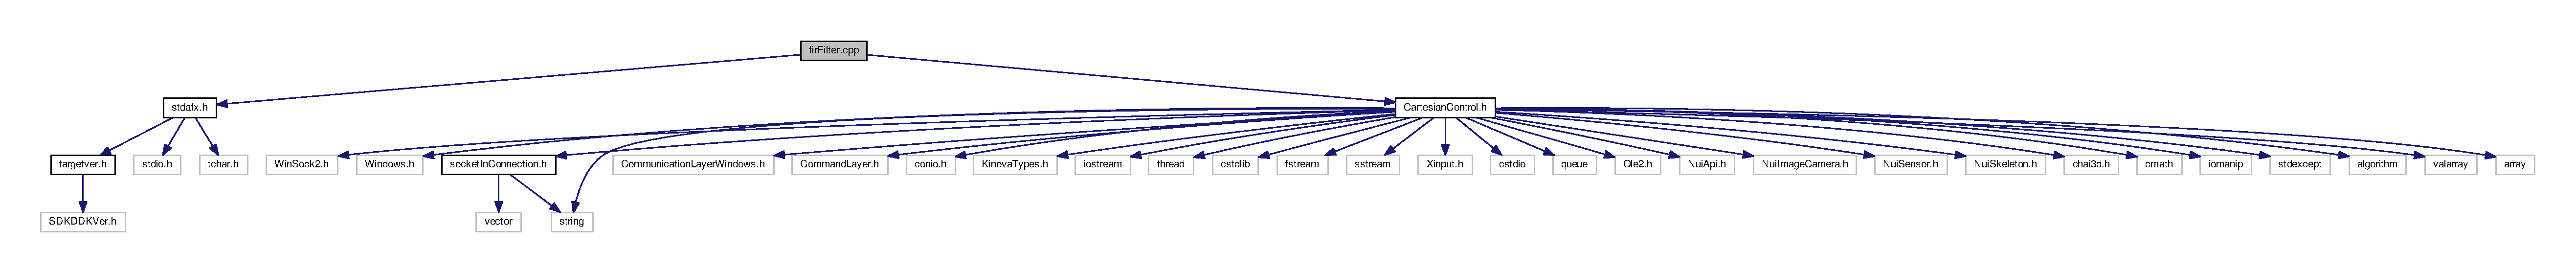
\includegraphics[width=350pt]{d2/d68/firFilter_8cpp__incl}
\end{center}
\end{figure}
\subsection*{Macros}
\begin{DoxyCompactItemize}
\item 
\#define \hyperlink{firFilter_8cpp_adfc8f90f3a8caa8423099cf36ff214f1}{\+\_\+\+W\+I\+N\+S\+O\+C\+K\+\_\+\+D\+E\+P\+R\+E\+C\+A\+T\+E\+D\+\_\+\+N\+O\+\_\+\+W\+A\+R\+N\+I\+N\+GS}
\end{DoxyCompactItemize}


\subsection{Macro Definition Documentation}
\index{fir\+Filter.\+cpp@{fir\+Filter.\+cpp}!\+\_\+\+W\+I\+N\+S\+O\+C\+K\+\_\+\+D\+E\+P\+R\+E\+C\+A\+T\+E\+D\+\_\+\+N\+O\+\_\+\+W\+A\+R\+N\+I\+N\+GS@{\+\_\+\+W\+I\+N\+S\+O\+C\+K\+\_\+\+D\+E\+P\+R\+E\+C\+A\+T\+E\+D\+\_\+\+N\+O\+\_\+\+W\+A\+R\+N\+I\+N\+GS}}
\index{\+\_\+\+W\+I\+N\+S\+O\+C\+K\+\_\+\+D\+E\+P\+R\+E\+C\+A\+T\+E\+D\+\_\+\+N\+O\+\_\+\+W\+A\+R\+N\+I\+N\+GS@{\+\_\+\+W\+I\+N\+S\+O\+C\+K\+\_\+\+D\+E\+P\+R\+E\+C\+A\+T\+E\+D\+\_\+\+N\+O\+\_\+\+W\+A\+R\+N\+I\+N\+GS}!fir\+Filter.\+cpp@{fir\+Filter.\+cpp}}
\subsubsection[{\texorpdfstring{\+\_\+\+W\+I\+N\+S\+O\+C\+K\+\_\+\+D\+E\+P\+R\+E\+C\+A\+T\+E\+D\+\_\+\+N\+O\+\_\+\+W\+A\+R\+N\+I\+N\+GS}{_WINSOCK_DEPRECATED_NO_WARNINGS}}]{\setlength{\rightskip}{0pt plus 5cm}\#define \+\_\+\+W\+I\+N\+S\+O\+C\+K\+\_\+\+D\+E\+P\+R\+E\+C\+A\+T\+E\+D\+\_\+\+N\+O\+\_\+\+W\+A\+R\+N\+I\+N\+GS}\hypertarget{firFilter_8cpp_adfc8f90f3a8caa8423099cf36ff214f1}{}\label{firFilter_8cpp_adfc8f90f3a8caa8423099cf36ff214f1}

\hypertarget{HMIfunctions_8cpp}{}\section{H\+M\+Ifunctions.\+cpp File Reference}
\label{HMIfunctions_8cpp}\index{H\+M\+Ifunctions.\+cpp@{H\+M\+Ifunctions.\+cpp}}
{\ttfamily \#include \char`\"{}stdafx.\+h\char`\"{}}\\*
{\ttfamily \#include \char`\"{}Cartesian\+Control.\+h\char`\"{}}\\*
{\ttfamily \#include $<$future$>$}\\*
Include dependency graph for H\+M\+Ifunctions.\+cpp\+:\nopagebreak
\begin{figure}[H]
\begin{center}
\leavevmode
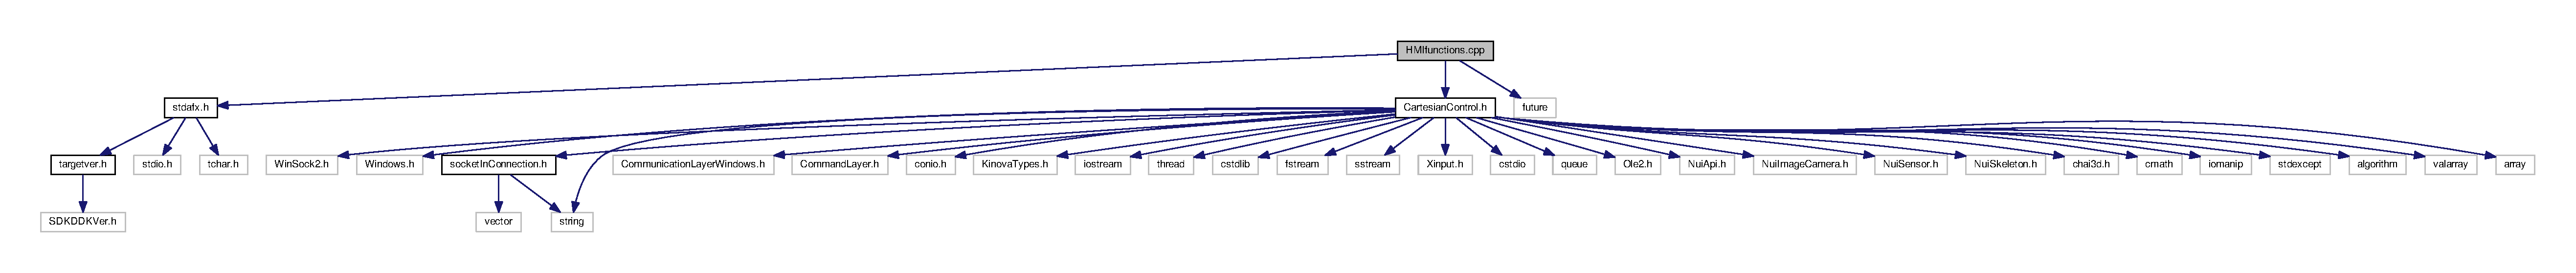
\includegraphics[width=350pt]{d9/d6d/HMIfunctions_8cpp__incl}
\end{center}
\end{figure}
\subsection*{Macros}
\begin{DoxyCompactItemize}
\item 
\#define \hyperlink{HMIfunctions_8cpp_adfc8f90f3a8caa8423099cf36ff214f1}{\+\_\+\+W\+I\+N\+S\+O\+C\+K\+\_\+\+D\+E\+P\+R\+E\+C\+A\+T\+E\+D\+\_\+\+N\+O\+\_\+\+W\+A\+R\+N\+I\+N\+GS}
\end{DoxyCompactItemize}


\subsection{Macro Definition Documentation}
\index{H\+M\+Ifunctions.\+cpp@{H\+M\+Ifunctions.\+cpp}!\+\_\+\+W\+I\+N\+S\+O\+C\+K\+\_\+\+D\+E\+P\+R\+E\+C\+A\+T\+E\+D\+\_\+\+N\+O\+\_\+\+W\+A\+R\+N\+I\+N\+GS@{\+\_\+\+W\+I\+N\+S\+O\+C\+K\+\_\+\+D\+E\+P\+R\+E\+C\+A\+T\+E\+D\+\_\+\+N\+O\+\_\+\+W\+A\+R\+N\+I\+N\+GS}}
\index{\+\_\+\+W\+I\+N\+S\+O\+C\+K\+\_\+\+D\+E\+P\+R\+E\+C\+A\+T\+E\+D\+\_\+\+N\+O\+\_\+\+W\+A\+R\+N\+I\+N\+GS@{\+\_\+\+W\+I\+N\+S\+O\+C\+K\+\_\+\+D\+E\+P\+R\+E\+C\+A\+T\+E\+D\+\_\+\+N\+O\+\_\+\+W\+A\+R\+N\+I\+N\+GS}!H\+M\+Ifunctions.\+cpp@{H\+M\+Ifunctions.\+cpp}}
\subsubsection[{\texorpdfstring{\+\_\+\+W\+I\+N\+S\+O\+C\+K\+\_\+\+D\+E\+P\+R\+E\+C\+A\+T\+E\+D\+\_\+\+N\+O\+\_\+\+W\+A\+R\+N\+I\+N\+GS}{_WINSOCK_DEPRECATED_NO_WARNINGS}}]{\setlength{\rightskip}{0pt plus 5cm}\#define \+\_\+\+W\+I\+N\+S\+O\+C\+K\+\_\+\+D\+E\+P\+R\+E\+C\+A\+T\+E\+D\+\_\+\+N\+O\+\_\+\+W\+A\+R\+N\+I\+N\+GS}\hypertarget{HMIfunctions_8cpp_adfc8f90f3a8caa8423099cf36ff214f1}{}\label{HMIfunctions_8cpp_adfc8f90f3a8caa8423099cf36ff214f1}

\hypertarget{KinovaHMICartesianControl_8cpp}{}\section{Kinova\+H\+M\+I\+Cartesian\+Control.\+cpp File Reference}
\label{KinovaHMICartesianControl_8cpp}\index{Kinova\+H\+M\+I\+Cartesian\+Control.\+cpp@{Kinova\+H\+M\+I\+Cartesian\+Control.\+cpp}}
{\ttfamily \#include \char`\"{}Cartesian\+Control.\+h\char`\"{}}\\*
Include dependency graph for Kinova\+H\+M\+I\+Cartesian\+Control.\+cpp\+:\nopagebreak
\begin{figure}[H]
\begin{center}
\leavevmode
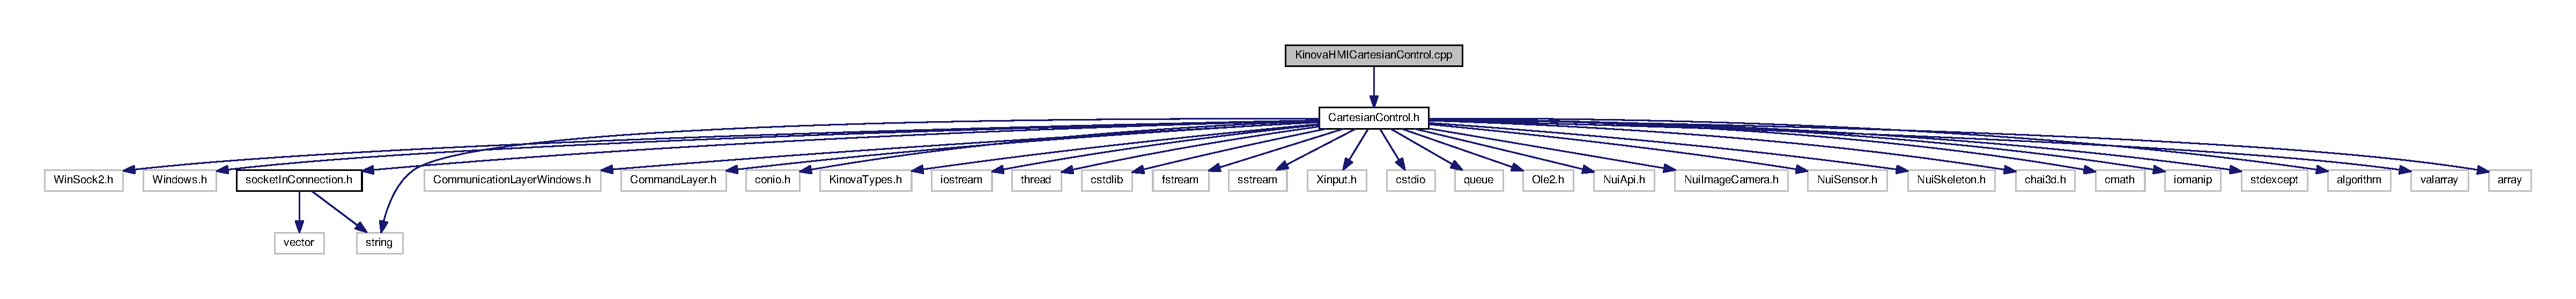
\includegraphics[width=350pt]{da/d8f/KinovaHMICartesianControl_8cpp__incl}
\end{center}
\end{figure}
\subsection*{Functions}
\begin{DoxyCompactItemize}
\item 
int \hyperlink{KinovaHMICartesianControl_8cpp_a0ddf1224851353fc92bfbff6f499fa97}{main} (int argc, char $\ast$argv\mbox{[}$\,$\mbox{]})
\end{DoxyCompactItemize}
\subsection*{Variables}
\begin{DoxyCompactItemize}
\item 
 H\+I\+N\+S\+T\+A\+N\+CE \hyperlink{KinovaHMICartesianControl_8cpp_a7dcbafc298af1cba5defa0baf9cfb948}{command\+Layer\+\_\+handle}
\end{DoxyCompactItemize}


\subsection{Function Documentation}
\index{Kinova\+H\+M\+I\+Cartesian\+Control.\+cpp@{Kinova\+H\+M\+I\+Cartesian\+Control.\+cpp}!main@{main}}
\index{main@{main}!Kinova\+H\+M\+I\+Cartesian\+Control.\+cpp@{Kinova\+H\+M\+I\+Cartesian\+Control.\+cpp}}
\subsubsection[{\texorpdfstring{main(int argc, char $\ast$argv[])}{main(int argc, char *argv[])}}]{\setlength{\rightskip}{0pt plus 5cm}int main (
\begin{DoxyParamCaption}
\item[{int}]{argc, }
\item[{char $\ast$}]{argv\mbox{[}$\,$\mbox{]}}
\end{DoxyParamCaption}
)}\hypertarget{KinovaHMICartesianControl_8cpp_a0ddf1224851353fc92bfbff6f499fa97}{}\label{KinovaHMICartesianControl_8cpp_a0ddf1224851353fc92bfbff6f499fa97}


\subsection{Variable Documentation}
\index{Kinova\+H\+M\+I\+Cartesian\+Control.\+cpp@{Kinova\+H\+M\+I\+Cartesian\+Control.\+cpp}!command\+Layer\+\_\+handle@{command\+Layer\+\_\+handle}}
\index{command\+Layer\+\_\+handle@{command\+Layer\+\_\+handle}!Kinova\+H\+M\+I\+Cartesian\+Control.\+cpp@{Kinova\+H\+M\+I\+Cartesian\+Control.\+cpp}}
\subsubsection[{\texorpdfstring{command\+Layer\+\_\+handle}{commandLayer_handle}}]{\setlength{\rightskip}{0pt plus 5cm} H\+I\+N\+S\+T\+A\+N\+CE command\+Layer\+\_\+handle}\hypertarget{KinovaHMICartesianControl_8cpp_a7dcbafc298af1cba5defa0baf9cfb948}{}\label{KinovaHMICartesianControl_8cpp_a7dcbafc298af1cba5defa0baf9cfb948}

\hypertarget{lutLinearInterp_8cpp}{}\section{lut\+Linear\+Interp.\+cpp File Reference}
\label{lutLinearInterp_8cpp}\index{lut\+Linear\+Interp.\+cpp@{lut\+Linear\+Interp.\+cpp}}
{\ttfamily \#include \char`\"{}stdafx.\+h\char`\"{}}\\*
{\ttfamily \#include \char`\"{}Cartesian\+Control.\+h\char`\"{}}\\*
Include dependency graph for lut\+Linear\+Interp.\+cpp\+:\nopagebreak
\begin{figure}[H]
\begin{center}
\leavevmode
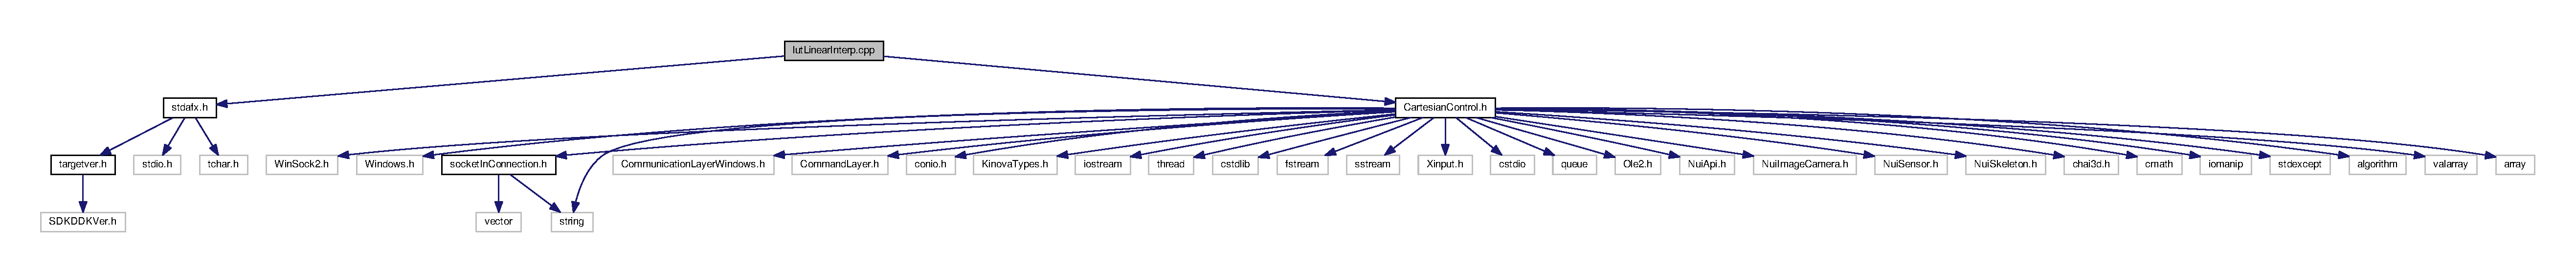
\includegraphics[width=350pt]{dc/d54/lutLinearInterp_8cpp__incl}
\end{center}
\end{figure}
\subsection*{Macros}
\begin{DoxyCompactItemize}
\item 
\#define \hyperlink{lutLinearInterp_8cpp_adfc8f90f3a8caa8423099cf36ff214f1}{\+\_\+\+W\+I\+N\+S\+O\+C\+K\+\_\+\+D\+E\+P\+R\+E\+C\+A\+T\+E\+D\+\_\+\+N\+O\+\_\+\+W\+A\+R\+N\+I\+N\+GS}
\item 
\#define \hyperlink{lutLinearInterp_8cpp_ac7bef5d85e3dcd73eef56ad39ffc84a9}{W\+I\+N32\+\_\+\+L\+E\+A\+N\+\_\+\+A\+N\+D\+\_\+\+M\+E\+AN}
\end{DoxyCompactItemize}


\subsection{Macro Definition Documentation}
\index{lut\+Linear\+Interp.\+cpp@{lut\+Linear\+Interp.\+cpp}!\+\_\+\+W\+I\+N\+S\+O\+C\+K\+\_\+\+D\+E\+P\+R\+E\+C\+A\+T\+E\+D\+\_\+\+N\+O\+\_\+\+W\+A\+R\+N\+I\+N\+GS@{\+\_\+\+W\+I\+N\+S\+O\+C\+K\+\_\+\+D\+E\+P\+R\+E\+C\+A\+T\+E\+D\+\_\+\+N\+O\+\_\+\+W\+A\+R\+N\+I\+N\+GS}}
\index{\+\_\+\+W\+I\+N\+S\+O\+C\+K\+\_\+\+D\+E\+P\+R\+E\+C\+A\+T\+E\+D\+\_\+\+N\+O\+\_\+\+W\+A\+R\+N\+I\+N\+GS@{\+\_\+\+W\+I\+N\+S\+O\+C\+K\+\_\+\+D\+E\+P\+R\+E\+C\+A\+T\+E\+D\+\_\+\+N\+O\+\_\+\+W\+A\+R\+N\+I\+N\+GS}!lut\+Linear\+Interp.\+cpp@{lut\+Linear\+Interp.\+cpp}}
\subsubsection[{\texorpdfstring{\+\_\+\+W\+I\+N\+S\+O\+C\+K\+\_\+\+D\+E\+P\+R\+E\+C\+A\+T\+E\+D\+\_\+\+N\+O\+\_\+\+W\+A\+R\+N\+I\+N\+GS}{_WINSOCK_DEPRECATED_NO_WARNINGS}}]{\setlength{\rightskip}{0pt plus 5cm}\#define \+\_\+\+W\+I\+N\+S\+O\+C\+K\+\_\+\+D\+E\+P\+R\+E\+C\+A\+T\+E\+D\+\_\+\+N\+O\+\_\+\+W\+A\+R\+N\+I\+N\+GS}\hypertarget{lutLinearInterp_8cpp_adfc8f90f3a8caa8423099cf36ff214f1}{}\label{lutLinearInterp_8cpp_adfc8f90f3a8caa8423099cf36ff214f1}
\index{lut\+Linear\+Interp.\+cpp@{lut\+Linear\+Interp.\+cpp}!W\+I\+N32\+\_\+\+L\+E\+A\+N\+\_\+\+A\+N\+D\+\_\+\+M\+E\+AN@{W\+I\+N32\+\_\+\+L\+E\+A\+N\+\_\+\+A\+N\+D\+\_\+\+M\+E\+AN}}
\index{W\+I\+N32\+\_\+\+L\+E\+A\+N\+\_\+\+A\+N\+D\+\_\+\+M\+E\+AN@{W\+I\+N32\+\_\+\+L\+E\+A\+N\+\_\+\+A\+N\+D\+\_\+\+M\+E\+AN}!lut\+Linear\+Interp.\+cpp@{lut\+Linear\+Interp.\+cpp}}
\subsubsection[{\texorpdfstring{W\+I\+N32\+\_\+\+L\+E\+A\+N\+\_\+\+A\+N\+D\+\_\+\+M\+E\+AN}{WIN32_LEAN_AND_MEAN}}]{\setlength{\rightskip}{0pt plus 5cm}\#define W\+I\+N32\+\_\+\+L\+E\+A\+N\+\_\+\+A\+N\+D\+\_\+\+M\+E\+AN}\hypertarget{lutLinearInterp_8cpp_ac7bef5d85e3dcd73eef56ad39ffc84a9}{}\label{lutLinearInterp_8cpp_ac7bef5d85e3dcd73eef56ad39ffc84a9}

\hypertarget{socketInConnection_8cpp}{}\section{socket\+In\+Connection.\+cpp File Reference}
\label{socketInConnection_8cpp}\index{socket\+In\+Connection.\+cpp@{socket\+In\+Connection.\+cpp}}
{\ttfamily \#include \char`\"{}stdafx.\+h\char`\"{}}\\*
{\ttfamily \#include \char`\"{}socket\+In\+Connection.\+h\char`\"{}}\\*
{\ttfamily \#include \char`\"{}Cartesian\+Control.\+h\char`\"{}}\\*
Include dependency graph for socket\+In\+Connection.\+cpp\+:\nopagebreak
\begin{figure}[H]
\begin{center}
\leavevmode
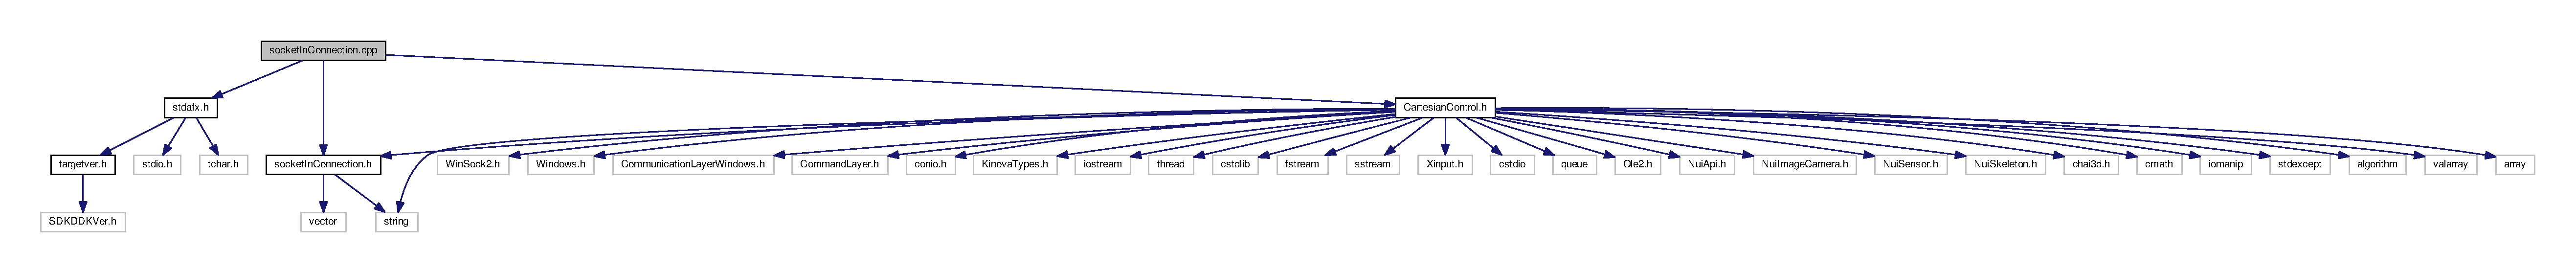
\includegraphics[width=350pt]{da/d9d/socketInConnection_8cpp__incl}
\end{center}
\end{figure}
\subsection*{Macros}
\begin{DoxyCompactItemize}
\item 
\#define \hyperlink{socketInConnection_8cpp_adfc8f90f3a8caa8423099cf36ff214f1}{\+\_\+\+W\+I\+N\+S\+O\+C\+K\+\_\+\+D\+E\+P\+R\+E\+C\+A\+T\+E\+D\+\_\+\+N\+O\+\_\+\+W\+A\+R\+N\+I\+N\+GS}
\item 
\#define \hyperlink{socketInConnection_8cpp_acaf400df9a74b3295697ca29cc9261cb}{H\+E\+A\+D\+E\+R\+\_\+\+L\+E\+N\+G\+TH}~6
\end{DoxyCompactItemize}


\subsection{Macro Definition Documentation}
\index{socket\+In\+Connection.\+cpp@{socket\+In\+Connection.\+cpp}!\+\_\+\+W\+I\+N\+S\+O\+C\+K\+\_\+\+D\+E\+P\+R\+E\+C\+A\+T\+E\+D\+\_\+\+N\+O\+\_\+\+W\+A\+R\+N\+I\+N\+GS@{\+\_\+\+W\+I\+N\+S\+O\+C\+K\+\_\+\+D\+E\+P\+R\+E\+C\+A\+T\+E\+D\+\_\+\+N\+O\+\_\+\+W\+A\+R\+N\+I\+N\+GS}}
\index{\+\_\+\+W\+I\+N\+S\+O\+C\+K\+\_\+\+D\+E\+P\+R\+E\+C\+A\+T\+E\+D\+\_\+\+N\+O\+\_\+\+W\+A\+R\+N\+I\+N\+GS@{\+\_\+\+W\+I\+N\+S\+O\+C\+K\+\_\+\+D\+E\+P\+R\+E\+C\+A\+T\+E\+D\+\_\+\+N\+O\+\_\+\+W\+A\+R\+N\+I\+N\+GS}!socket\+In\+Connection.\+cpp@{socket\+In\+Connection.\+cpp}}
\subsubsection[{\texorpdfstring{\+\_\+\+W\+I\+N\+S\+O\+C\+K\+\_\+\+D\+E\+P\+R\+E\+C\+A\+T\+E\+D\+\_\+\+N\+O\+\_\+\+W\+A\+R\+N\+I\+N\+GS}{_WINSOCK_DEPRECATED_NO_WARNINGS}}]{\setlength{\rightskip}{0pt plus 5cm}\#define \+\_\+\+W\+I\+N\+S\+O\+C\+K\+\_\+\+D\+E\+P\+R\+E\+C\+A\+T\+E\+D\+\_\+\+N\+O\+\_\+\+W\+A\+R\+N\+I\+N\+GS}\hypertarget{socketInConnection_8cpp_adfc8f90f3a8caa8423099cf36ff214f1}{}\label{socketInConnection_8cpp_adfc8f90f3a8caa8423099cf36ff214f1}
\index{socket\+In\+Connection.\+cpp@{socket\+In\+Connection.\+cpp}!H\+E\+A\+D\+E\+R\+\_\+\+L\+E\+N\+G\+TH@{H\+E\+A\+D\+E\+R\+\_\+\+L\+E\+N\+G\+TH}}
\index{H\+E\+A\+D\+E\+R\+\_\+\+L\+E\+N\+G\+TH@{H\+E\+A\+D\+E\+R\+\_\+\+L\+E\+N\+G\+TH}!socket\+In\+Connection.\+cpp@{socket\+In\+Connection.\+cpp}}
\subsubsection[{\texorpdfstring{H\+E\+A\+D\+E\+R\+\_\+\+L\+E\+N\+G\+TH}{HEADER_LENGTH}}]{\setlength{\rightskip}{0pt plus 5cm}\#define H\+E\+A\+D\+E\+R\+\_\+\+L\+E\+N\+G\+TH~6}\hypertarget{socketInConnection_8cpp_acaf400df9a74b3295697ca29cc9261cb}{}\label{socketInConnection_8cpp_acaf400df9a74b3295697ca29cc9261cb}

\hypertarget{socketInConnection_8h}{}\section{socket\+In\+Connection.\+h File Reference}
\label{socketInConnection_8h}\index{socket\+In\+Connection.\+h@{socket\+In\+Connection.\+h}}
{\ttfamily \#include $<$vector$>$}\\*
{\ttfamily \#include $<$string$>$}\\*
Include dependency graph for socket\+In\+Connection.\+h\+:\nopagebreak
\begin{figure}[H]
\begin{center}
\leavevmode
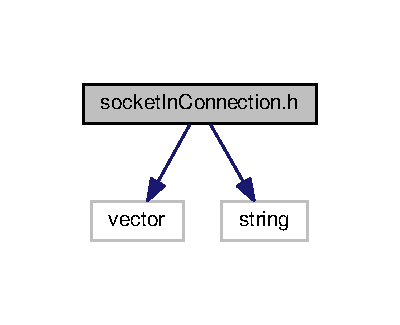
\includegraphics[width=192pt]{da/d1a/socketInConnection_8h__incl}
\end{center}
\end{figure}
This graph shows which files directly or indirectly include this file\+:\nopagebreak
\begin{figure}[H]
\begin{center}
\leavevmode
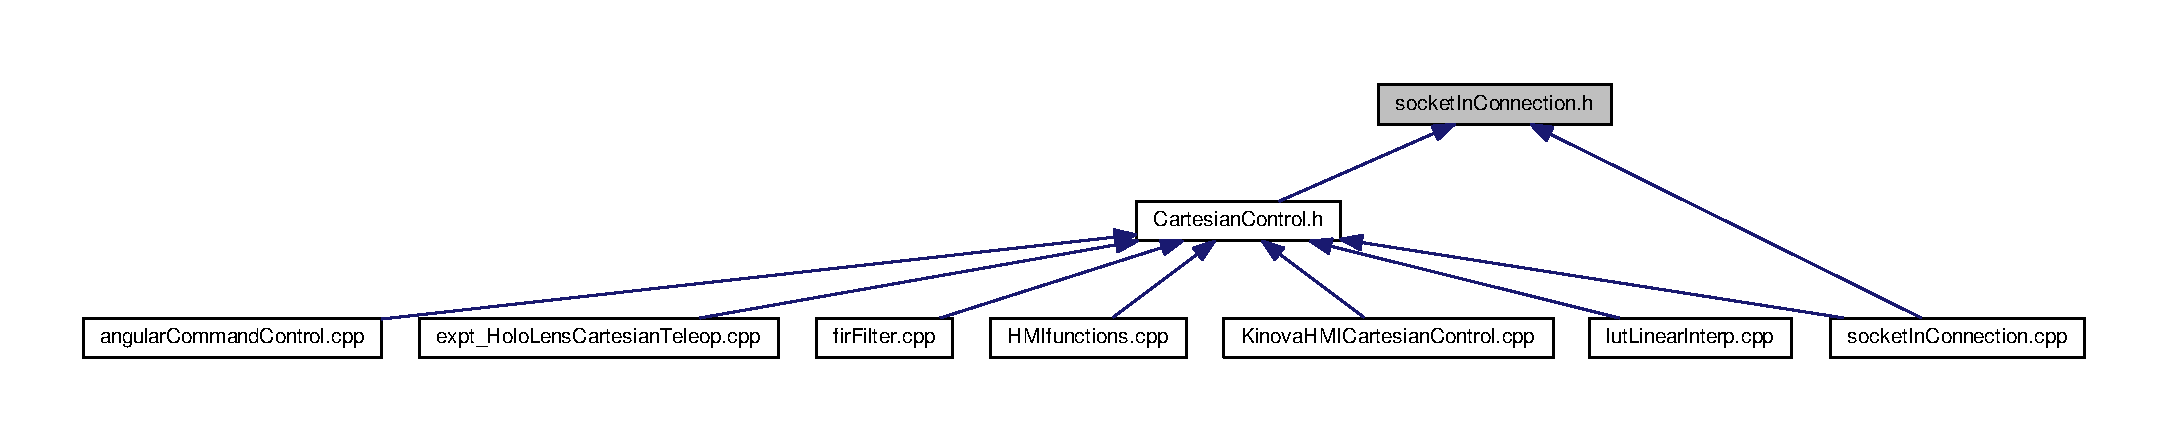
\includegraphics[width=350pt]{d2/d93/socketInConnection_8h__dep__incl}
\end{center}
\end{figure}
\subsection*{Classes}
\begin{DoxyCompactItemize}
\item 
class \hyperlink{classCSocketInConnection}{C\+Socket\+In\+Connection}
\end{DoxyCompactItemize}

\hypertarget{socketOutConnection_8h}{}\section{socket\+Out\+Connection.\+h File Reference}
\label{socketOutConnection_8h}\index{socket\+Out\+Connection.\+h@{socket\+Out\+Connection.\+h}}
{\ttfamily \#include $<$vector$>$}\\*
{\ttfamily \#include $<$string$>$}\\*
Include dependency graph for socket\+Out\+Connection.\+h\+:\nopagebreak
\begin{figure}[H]
\begin{center}
\leavevmode
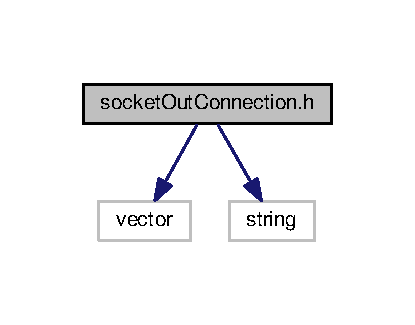
\includegraphics[width=199pt]{df/d2e/socketOutConnection_8h__incl}
\end{center}
\end{figure}
\subsection*{Classes}
\begin{DoxyCompactItemize}
\item 
class \hyperlink{classCSocketOutConnection}{C\+Socket\+Out\+Connection}
\end{DoxyCompactItemize}

\hypertarget{stdafx_8cpp}{}\section{stdafx.\+cpp File Reference}
\label{stdafx_8cpp}\index{stdafx.\+cpp@{stdafx.\+cpp}}
{\ttfamily \#include \char`\"{}stdafx.\+h\char`\"{}}\\*
Include dependency graph for stdafx.\+cpp\+:\nopagebreak
\begin{figure}[H]
\begin{center}
\leavevmode
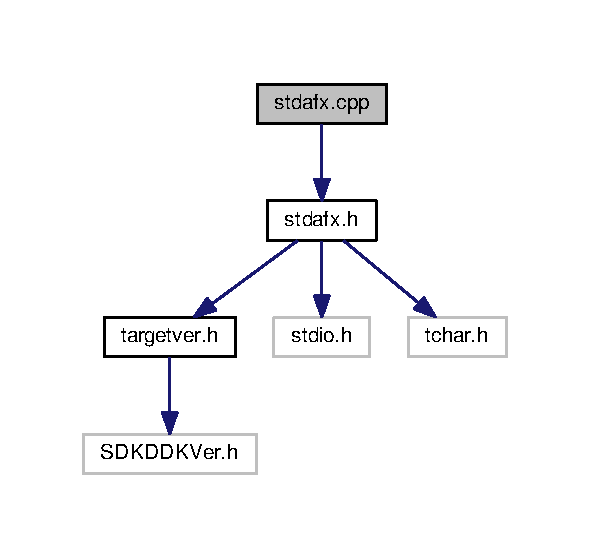
\includegraphics[width=283pt]{de/d79/stdafx_8cpp__incl}
\end{center}
\end{figure}

\hypertarget{stdafx_8h}{}\section{stdafx.\+h File Reference}
\label{stdafx_8h}\index{stdafx.\+h@{stdafx.\+h}}
{\ttfamily \#include \char`\"{}targetver.\+h\char`\"{}}\\*
{\ttfamily \#include $<$stdio.\+h$>$}\\*
{\ttfamily \#include $<$tchar.\+h$>$}\\*
Include dependency graph for stdafx.\+h\+:\nopagebreak
\begin{figure}[H]
\begin{center}
\leavevmode
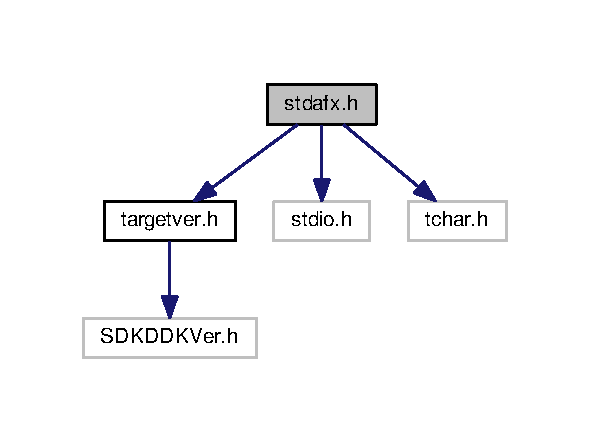
\includegraphics[width=283pt]{d5/da1/stdafx_8h__incl}
\end{center}
\end{figure}
This graph shows which files directly or indirectly include this file\+:\nopagebreak
\begin{figure}[H]
\begin{center}
\leavevmode
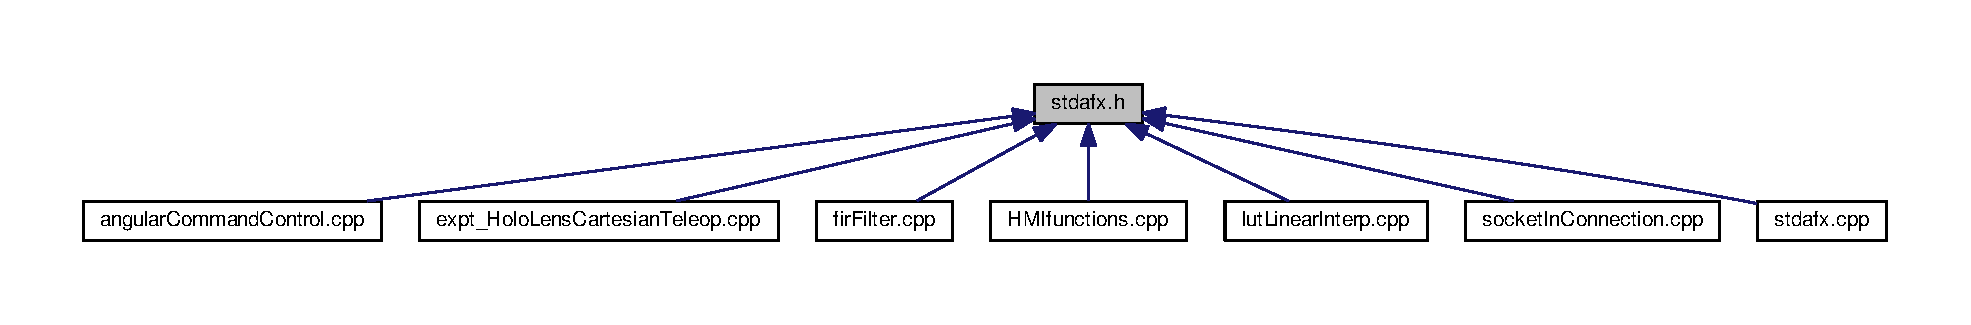
\includegraphics[width=350pt]{d3/d1b/stdafx_8h__dep__incl}
\end{center}
\end{figure}

\hypertarget{targetver_8h}{}\section{targetver.\+h File Reference}
\label{targetver_8h}\index{targetver.\+h@{targetver.\+h}}
{\ttfamily \#include $<$S\+D\+K\+D\+D\+K\+Ver.\+h$>$}\\*
Include dependency graph for targetver.\+h\+:\nopagebreak
\begin{figure}[H]
\begin{center}
\leavevmode
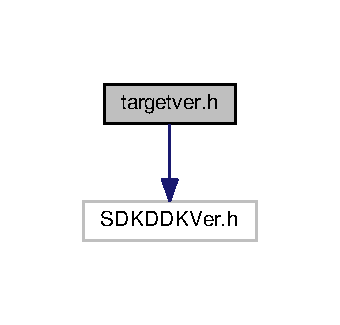
\includegraphics[width=163pt]{d4/dfa/targetver_8h__incl}
\end{center}
\end{figure}
This graph shows which files directly or indirectly include this file\+:\nopagebreak
\begin{figure}[H]
\begin{center}
\leavevmode
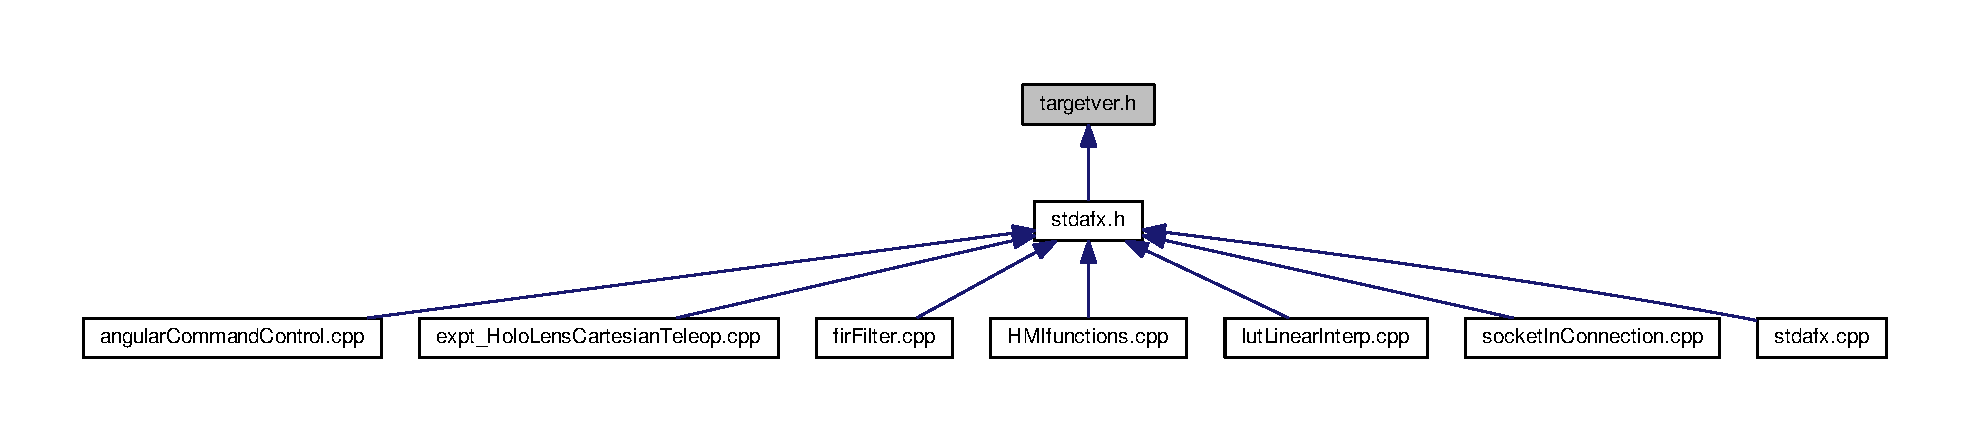
\includegraphics[width=350pt]{dc/dce/targetver_8h__dep__incl}
\end{center}
\end{figure}

%--- End generated contents ---

% Index
\backmatter
\newpage
\phantomsection
\clearemptydoublepage
\addcontentsline{toc}{chapter}{Index}
\printindex

\end{document}
